\documentclass[12pt, a4paper]{article}

\usepackage[utf8]{inputenc}
\usepackage[T1]{fontenc}
\usepackage{mathptmx}
\usepackage[margin=1in]{geometry}
\usepackage{graphicx}
\usepackage{booktabs}
\usepackage{amsmath}
\usepackage{amssymb}
\usepackage{amsthm}
\newtheorem{theorem}{Theorem}
\newtheorem{proposition}{Proposition}
\newtheorem{definition}{Definition}
\newtheorem{lemma}{Lemma}
\newtheorem*{remark}{Remark}
\usepackage{hyperref}
\usepackage{natbib}
\usepackage{caption}
\captionsetup{font=small}
\usepackage{subcaption}
\usepackage{float}
\usepackage{xcolor}
\usepackage{setspace}
\usepackage{titlesec}
\usepackage{placeins}
\usepackage{tikz}
\usetikzlibrary{positioning, fit, calc, arrows.meta, decorations.pathreplacing}
\usepackage{pgfplots}
\pgfplotsset{compat=1.18}
\usepgfplotslibrary{groupplots, fillbetween}

\definecolor{cblue}{HTML}{4477AA}
\definecolor{cgreen}{HTML}{228833}
\definecolor{cyellow}{HTML}{CCBB44}
\definecolor{cred}{HTML}{EE6677}
\definecolor{cmagenta}{HTML}{AA3377}
\definecolor{cgray}{HTML}{BBBBBB}
\definecolor{cdark}{HTML}{222222}

\pgfplotsset{gat/.style={
  width=\linewidth, height=0.42\linewidth,
  scale only axis,
  axis lines*=left,
  tick align=outside, tick pos=left,
  label style={font=\small},
  tick label style={font=\scriptsize},
  legend style={draw=none, fill=none, font=\scriptsize},
  legend cell align={left},
  every axis plot/.append style={line width=0.9pt},
  scaled ticks=false,
  /pgf/number format/fixed,
  /pgf/number format/precision=2,
}}
\titleformat{\section}{\normalsize\bfseries}{\thesection}{1em}{}
\titleformat{\subsection}{\normalsize\bfseries}{\thesubsection}{1em}{}
\titleformat{\subsubsection}{\normalsize\bfseries}{\thesubsubsection}{1em}{}
\titlespacing*{\section}{0pt}{12pt}{6pt}
\titlespacing*{\subsection}{0pt}{10pt}{4pt}
\titlespacing*{\subsubsection}{0pt}{8pt}{4pt}

\hypersetup{
    colorlinks=true,
    linkcolor=blue!70!black,
    citecolor=blue!70!black,
    urlcolor=blue!70!black
}

\onehalfspacing

\setlength{\intextsep}{4pt plus 2pt minus 2pt}
\setlength{\floatsep}{4pt plus 2pt minus 2pt}
\setlength{\textfloatsep}{6pt plus 2pt minus 4pt}
\setlength{\abovecaptionskip}{4pt}
\setlength{\belowcaptionskip}{2pt}
\renewcommand{\topfraction}{0.9}
\renewcommand{\bottomfraction}{0.9}
\renewcommand{\textfraction}{0.1}
\renewcommand{\floatpagefraction}{0.8}
\setcounter{topnumber}{3}
\setcounter{bottomnumber}{3}
\setcounter{totalnumber}{5}

\title{\textbf{The Geometry of Gridlock: Tracking Congressional Polarization\\ Through Spectral Analysis of Co-Voting Networks}}

\author{Jacob Crainic}

\date{}

\begin{document}
\raggedbottom

\maketitle

\begin{abstract}
The collapse of cross-party cooperation in the U.S. House after 2010 admits two competing explanations. The compositional account holds that more ideologically extreme legislators were elected, and the environmental account holds that the chamber's coalition architecture lost its capacity to absorb moderate members. Existing measures of congressional polarization rely on spatial scaling of roll-call votes and capture ideological divergence without speaking to either mechanism. We construct co-voting networks for every House Congress from the 100th through the 118th, develop spectral measures of bridging capacity, and adjudicate between the two accounts. The Bridge Legislator Index, defined as a node's contribution to the algebraic connectivity of the co-voting graph, admits a first-order closed form derived through Kato perturbation theory and recovers planted bridge nodes in stochastic block models more reliably than seven standard centralities across 17,280 graphs. Within Congress, a difference-in-difference-in-differences design and a death-in-office natural experiment identify the post-2010 collapse as environmental rather than compositional. Mediation analysis estimates that ideological centrism mediates roughly 95 percent of the Bridge Legislator Index relationship with legislator departure. The cooperative architecture documented here is structurally fragile and has not recovered.
\end{abstract}

\section{Introduction}

In October 2013, the Affordable Care Act had been law for three years and had survived a Supreme Court challenge, a presidential election, and forty-two separate House repeal votes. A faction of House Republicans nonetheless refused to fund the government unless the law was defunded, and the resulting sixteen-day shutdown furloughed 800,000 federal employees and cost the economy an estimated 24 billion dollars \citep{cbo2013}. The vote that ended it split almost perfectly along party lines. Episodes of this kind have become routine over the past decade, and political scientists have largely converged on a description of why. The two parties have moved further apart in ideological space, the moderate center of both parties has thinned, and the elementary mechanics of bipartisan cooperation have weakened. By the 114th Congress, the most liberal Republican in the House was more conservative than the most conservative Democrat, a pattern with no precedent in the modern era \citep{poole2017}.

What the field has not settled is the mechanism. One account is compositional. The legislators elected to the post-2010 House were more ideologically extreme than their predecessors, and the chamber's polarization is the aggregation of their individual positions. A second account is environmental. The chamber's coalition architecture, the residual scaffolding through which moderates of one party once found agreement with moderates of the other, collapsed in a way that prevented even similarly positioned incoming members from rebuilding cross-party ties. The two accounts predict different empirical signatures and recommend different responses, and they are not yet distinguishable with the measurement tools the field uses. The methodology gap is more than expository: spatial scaling treats each legislator as an independent point and discards the relational information through which the environmental story would have to operate.

The dominant framework for measuring congressional ideology is DW-NOMINATE, a scaling method that places legislators on a left-right continuum based on their roll-call votes \citep{poole1985, poole2017}. It has been enormously productive. The widening party distance since the 1970s is among the most robust empirical findings in American politics, and a generation of work has fitted ideal points to roll calls at increasingly fine resolution. NOMINATE is nevertheless a spatial model. It embeds legislators as independent points and votes as cutting lines, captures ideological position cleanly, and discards the relational structure of who cooperates with whom. This is the level at which a compositional-versus-environmental adjudication has to happen, and the level at which spatial scaling has nothing to say.

A network-analytic literature emerged in the early 2000s to recover what scaling discards. \citet{fowler2006a} constructed cosponsorship networks and showed that legislative connectedness predicts bill passage. \citet{waugh2009} applied modularity measures to co-voting networks and documented increasing partisan clustering. \citet{andris2015} produced striking visualizations of the near-complete disappearance of cross-party edges between the 1980s and 2010s, and \citet{aref2020} formalized coalition detection as optimal partitioning of signed networks. These contributions established that network structure carries information beyond what spatial models capture. They did not, however, supply a node-level measure of how much each member's removal would change the algebraic connectivity of the network, a closed-form theoretical characterization of such a measure, or a causal identification strategy that could distinguish compositional from environmental explanations of the post-2010 collapse.

In this article, we develop the spectral and causal tools needed to adjudicate that distinction. We construct co-voting networks for every House Congress from the 100th through the 118th, define the Bridge Legislator Index as a member's leave-one-out contribution to the second-smallest eigenvalue of the normalized graph Laplacian, prove a first-order approximation that recovers it from the Fiedler vector through Kato analytic perturbation theory, and demonstrate that it identifies planted bridge nodes in stochastic block models more reliably than seven standard centralities across 17,280 graphs spanning $K \in \{2, 3, 5, 10\}$ blocs and graph sizes from 105 to 2,020. Within Congress, we adjudicate the compositional-versus-environmental question with two designs. A cohort difference-in-difference-in-differences specification compares Tea Party freshmen to Contract with America freshmen against a competitive-district interaction, and a death-in-office natural experiment uses the exogenous removal of legislators as a leave-one-out experiment with Aronow-Samii exposure mappings. We extend the analysis to the U.S. Senate, run a bicameral synthetic difference-in-differences with the Senate as a quasi-control insulated by the filibuster, and use a battery of sensitivity analyses to bound the residual ambiguity in observational claims.

The findings are consistent with the environmental account. The cohort difference-in-difference-in-differences and the staggered Callaway-Sant'Anna across five electoral waves both identify the 2010 Tea Party Congress as the uniquely negative cohort. Mediation analysis through ideological centrism estimates that roughly 95 percent of the Bridge Legislator Index relationship with legislator departure operates through the centrism channel rather than directly through network position. The death-in-office identification shows that surviving co-voters of high-Bridge-Legislator-Index legislators increase their cross-party agreement by 5 to 6 percentage points relative to surviving co-voters of low-Bridge-Legislator-Index legislators. The bicameral comparison shows that the House's post-2010 Fiedler collapse is 0.33 larger than the Senate's, statistically distinguishable and consistent with the filibuster's structural incentive for cross-party cooperation. The remainder of the article is organized as follows. Section~2 reviews related work. Section~3 describes the data and graph construction. Section~4 presents the spectral analysis. Section~5 visualizes the network at the boundary of the collapse. Sections~6 and~7 introduce the Bridge Legislator Index and its theoretical properties. Sections~8 and~9 turn to causal identification and mediation. Section~10 supplies the counterfactual perturbation experiments, and Section~11 concludes.

\section{Related Work}

The dominant framework for measuring legislative ideology is DW-NOMINATE, a spatial scaling method that places legislators on a left-right continuum based on their roll-call votes \citep{poole1985, poole2017}. It has been enormously productive: the divergence of the two parties since the 1970s is among the most robust findings in American politics. But NOMINATE is fundamentally a spatial model. It embeds legislators as independent points and votes as cutting lines, capturing ideological position while discarding the relational structure of who cooperates with whom.

Recognizing this limitation, a network-analytic literature emerged in the early 2000s. \citet{fowler2006a} constructed co-sponsorship networks and found that legislative connectedness predicts bill passage. \citet{waugh2009} applied modularity measures to co-voting networks and documented increasing partisan clustering over time. \citet{andris2015} produced striking visualizations of the near-complete disappearance of cross-party edges between the 1980s and 2010s. These contributions established that network structure carries information beyond what spatial models capture. What remained missing was a formal framework connecting network topology to the mechanisms of polarization: the specific structural features that degrade, the members whose removal matters most, and the system's capacity to recover from shocks.

Spectral graph theory offers tools suited to this task. The Fiedler value, the second-smallest eigenvalue of the graph Laplacian, measures how close a network is to splitting into disconnected components \citep{fiedler1973}. \citet{newman2006} used spectral methods to identify partisan structure in congressional networks, and \citet{moody2013} traced the evolution of partisan clustering with related techniques. Our analysis extends this spectral tradition with a substantially longer time series, a novel node-level centrality measure grounded in the Fiedler value, and a formal statistical test linking bridge position to electoral vulnerability.

A natural alternative to spectral methods is stochastic block modeling (SBM), which identifies latent community structure from network data. In congressional networks, however, SBMs trivially recover party labels as the dominant partition. Our interest is not in detecting communities (which are known a priori) but in measuring the \textit{connectivity between} known communities, which is precisely what the Fiedler value captures. The BLI has no natural SBM analog: it measures individual contribution to inter-community connectivity rather than community membership probability. We therefore position spectral analysis as complementary to SBMs rather than competing with them.

On the political science side, \citet{theriault2008} documented how procedural changes accelerated partisan conflict, \citet{skocpol2012} analyzed the Tea Party as both grassroots movement and elite-driven realignment, and \citet{mann2012} argued that asymmetric polarization driven by the Republican Party's rightward shift is the dominant dynamic. These accounts offer complementary causal narratives. Our spectral time series and structural recovery analysis provide an independent, network-structural test of when and how sharply the cooperative architecture of Congress fractured, and whether the fractures proved reversible.

\section{Data and Graph Construction}\label{sec:data}

\subsection{Roll-Call Voting Records}

Roll-call voting records come from Voteview \citep{lewis2023}, covering the U.S. House of Representatives from the 100th Congress (1987--1989) through the 118th Congress (2023--2025). Each record indicates whether a member voted yea, nay, or did not vote. We filter to members affiliated with the two major parties and require a minimum of 50 recorded votes per member. This yields an average of 442 members per Congress across 19 Congresses, or approximately 8,400 member-Congress observations.

\subsection{Co-Voting Agreement Networks}

For each pair of members within a Congress, we compute a pairwise agreement score as the fraction of shared roll calls on which both cast the same vote. For members $i$ and $j$ who both voted on roll calls $\mathcal{R}_{ij}$:
\begin{equation}
    a_{ij} = \frac{|\{r \in \mathcal{R}_{ij} : v_i^r = v_j^r\}|}{|\mathcal{R}_{ij}|}
\end{equation}
where $v_i^r \in \{0, 1\}$ denotes the vote of member $i$ on roll call $r$. We require $|\mathcal{R}_{ij}| \geq 20$.

The agreement matrix $A$ is dense. Many votes are near-unanimous. We threshold at $\tau = 0.5$ to create an unweighted adjacency matrix $\hat{A}$ where an edge indicates agreement on a majority of shared votes. While we report our primary findings using an unweighted binary agreement threshold of $\tau = 0.5$ to establish clear topological boundaries, our findings regarding the collapse of the algebraic connectivity are not artifacts of this specific cutoff. The qualitative pattern of the Fiedler value deterioration remains highly stable across agreement thresholds ranging from $\tau = 0.4$ to $0.7$, as detailed in the sensitivity analysis in Appendix~\ref{app:threshold}.

\subsection{Node Features}

Each node has an eight-dimensional feature vector: DW-NOMINATE scores on both dimensions \citep{poole2017}, party affiliation, vote participation rate, yea-vote rate, mean agreement with all other members, mean cross-party agreement, and mean within-party agreement. These features characterize each legislator's voting profile and position within the co-voting network. In the departure analysis (Section~8), we use ideology scores, party affiliation, and seniority as covariates; the agreement-based features enter implicitly through the BLI, which is computed from the adjacency matrix they help define.

\section{Spectral Analysis}

\subsection{Algebraic Connectivity and Polarization}

The normalized graph Laplacian is $\mathcal{L} = I - D^{-1/2} \hat{A} D^{-1/2}$, where $D$ is the diagonal degree matrix. Its second-smallest eigenvalue, the Fiedler value $\lambda_2$, measures how well-connected the graph is. Values near zero indicate the graph is close to splitting into disconnected components; larger values indicate a more integrated structure \citep{fiedler1973}.

In the 100th Congress (1987), $\lambda_2$ stood at 0.534. By the 114th (2015), it had fallen to 0.010, a decline of over 98\%. The co-voting graph had, in structural terms, nearly split in two. Table~\ref{tab:polarization} summarizes these metrics across the study period.

\begin{table}[H]
\centering
\caption{Congressional polarization metrics across selected Congresses. The Fiedler value captures network connectivity; party distance measures ideological divergence. Both deteriorate, but at different rates and with different dynamics. The 111th Congress row is new to this analysis and reveals a previously undocumented connectivity spike.}
\label{tab:polarization}
\begin{tabular}{lcccccc}
\toprule
Congress & Years & Members & Fiedler & Party Dist. & Density & Mean Degree \\
\midrule
100th & 1987--89 & 439 & 0.534 & 0.666 & 0.780 & 341.6 \\
103rd & 1993--95 & 441 & 0.230 & 0.712 & 0.609 & 268.1 \\
107th & 2001--03 & 439 & 0.805 & 0.786 & 0.928 & 406.5 \\
111th & 2009--11 & 450 & 0.737 & 0.794 & 0.897 & 402.8 \\
112th & 2011--13 & 442 & 0.073 & 0.867 & 0.538 & 237.4 \\
114th & 2015--17 & 436 & 0.010 & 0.886 & 0.512 & 222.9 \\
117th & 2021--23 & 447 & 0.086 & 0.880 & 0.536 & 238.8 \\
118th & 2023--25 & 451 & 0.032 & 0.892 & 0.510 & 229.3 \\
\bottomrule
\end{tabular}
\end{table}

\subsection{Density Without Connectivity}

Density declines only modestly from 0.780 to 0.510 even as the Fiedler value collapses from 0.534 to 0.010 (Table~\ref{tab:polarization}). This disproportionality reveals that edges are not simply lost but reorganized: within-party connections densify while cross-party bridges vanish. The network retains most of its edges even as it structurally fractures. Polarization is a structural rewiring, not a loss of cooperation, and aggregate measures like density miss this entirely.

\subsection{Validation Against DW-NOMINATE}

The Fiedler value and DW-NOMINATE party distance both capture polarization, but they are not the same measure. Party distance tracks the separation between mean ideological positions; the Fiedler value tracks structural connectivity of the cooperation network. They correlate ($r = -0.76$, since lower Fiedler means more polarized), but the dynamics differ (Figure~\ref{fig:polarization}).

The most visible difference: the Fiedler value shows a sharp, non-monotonic trajectory. It rises from 0.534 in the 100th Congress to 0.805 in the 107th (2001--2003), then falls, surges again to 0.737 in the 111th (2009--2011), and collapses to near zero by the 113th. Party distance, by contrast, increases smoothly and monotonically. The network structure captures dynamics that ideological scaling misses: temporary surges in bipartisan cooperation and sudden structural breaks that get smoothed away in spatial models.

The 107th Congress deserves attention. A Fiedler value of 0.805 represents the most structurally connected House in our entire dataset, and it occurred when DW-NOMINATE party distance was already high (0.786). The explanation lies substantially in the post-9/11 rally effect: the Authorization for Use of Military Force passed the House 420--1, and a wave of national security legislation drew broad bipartisan support that temporarily rewired the co-voting graph. An important caveat: when restricted to substantive policy votes (excluding procedural motions and near-unanimous suspension bills), the 107th's Fiedler value drops from 0.805 to 0.210 (Appendix~\ref{app:vote_filter}). The post-9/11 cooperation surge was real but partially concentrated in suspension votes, which are bipartisan by design. The exogenous shock still produced a genuine structural deviation from the temporal null (Section~4.4), but the spike's magnitude on contested legislation was considerably more modest.

The 111th Congress (2009--2011) reveals a second connectivity spike. With a Fiedler value of 0.737 on all votes (0.110 on substantive votes only), the Obama supermajority Congress shows elevated bipartisan cooperation, again concentrated in suspension and procedural categories. The mechanism is not entirely clear. TARP was enacted in the 110th Congress (October 2008), not the 111th, and the Affordable Care Act passed on a party-line vote. One plausible explanation is that the large Democratic majority allowed conservative Democrats to defect on high-profile bills without endangering passage, creating cross-party voting patterns with Republicans on fiscal and defense legislation. A complementary factor is that the 111th Congress passed an unusually high volume of suspension bills (831 of 1,647 recorded votes), clearing a backlog of noncontroversial legislation before the anticipated 2010 midterm losses. Whatever the cause, the result on the full vote set is a striking oscillation: the Fiedler value swings from 0.238 (110th) to 0.737 (111th) to 0.073 (112th), a range of 0.664 in just two transitions. On substantive votes the oscillation is smaller (0.073 to 0.110 to 0.036) but the post-Tea Party collapse is, if anything, starker. The Tea Party wave did not merely continue a gradual decline; it shattered even the modest substantive cooperation that remained.

What happened after each connectivity peak is the key finding. The post-9/11 surge reversed within two Congresses, with the Fiedler value falling from 0.805 back below 0.5 by the 109th. The system snapped back. Now compare that to the post-2010 period: after the Tea Party wave drove connectivity from 0.737 to 0.073, no subsequent event produced anything resembling a recovery. Not the Trump presidency, not the January 6th crisis, not a global pandemic. The graph stayed disconnected. This asymmetry points to something beyond the level of polarization itself. In the early 2000s, a crisis could temporarily override partisan sorting and rebuild bipartisan cooperation. By the 2010s, that capacity appears to have been lost. The network cannot regenerate the cross-party connections that crises once produced.

\begin{figure}[H]
\centering
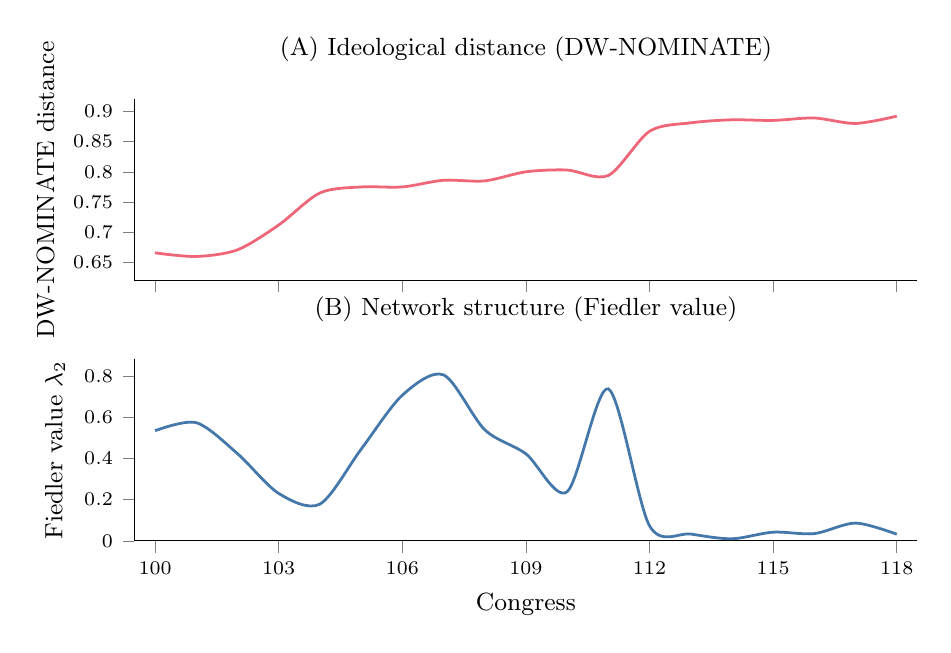
\begin{tikzpicture}
\begin{groupplot}[
  group style={
    group size=1 by 2,
    vertical sep=1.0cm,
    x descriptions at=edge bottom,
  },
  gat,
  width=0.82\linewidth, height=0.19\linewidth,
  xmin=99.5, xmax=118.5,
  xtick={100,103,106,109,112,115,118},
  enlargelimits=false,
]

\nextgroupplot[
  ymin=0.62, ymax=0.92,
  ytick={0.65,0.70,0.75,0.80,0.85,0.90},
  ylabel={DW-NOMINATE distance},
  title={(A) Ideological distance (DW-NOMINATE)},
  title style={font=\small, yshift=4pt},
]
\addplot[cred, smooth, tension=0.5, line width=1pt, mark=none]
  coordinates {
    (100,0.666) (101,0.660) (102,0.671) (103,0.712) (104,0.765)
    (105,0.775) (106,0.775) (107,0.786) (108,0.785) (109,0.800)
    (110,0.803) (111,0.794) (112,0.867) (113,0.881) (114,0.886)
    (115,0.885) (116,0.889) (117,0.880) (118,0.892)
  };

\nextgroupplot[
  ymin=0, ymax=0.88,
  ytick={0,0.2,0.4,0.6,0.8},
  ylabel={Fiedler value $\lambda_2$},
  xlabel={Congress},
  title={(B) Network structure (Fiedler value)},
  title style={font=\small, yshift=4pt},
]
\addplot[cblue, smooth, tension=0.5, line width=1pt, mark=none]
  coordinates {
    (100,0.534) (101,0.573) (102,0.423) (103,0.230) (104,0.178)
    (105,0.444) (106,0.706) (107,0.805) (108,0.539) (109,0.422)
    (110,0.238) (111,0.737) (112,0.073) (113,0.033) (114,0.010)
    (115,0.042) (116,0.035) (117,0.086) (118,0.032)
  };

\end{groupplot}
\end{tikzpicture}
\caption{Two measures of polarization across the 100th--118th Congresses. (A) DW-NOMINATE party distance, the canonical ideological-distance measure (range $[0.67, 0.89]$). (B) Fiedler value $\lambda_2$ of the co-voting network's normalized Laplacian (range $[0.01, 0.81]$). The two measures correlate at $r = -0.76$.}
\label{fig:polarization}
\end{figure}

\subsection{Spectral Gap and Partisan Bisection}

The two-bloc interpretation of the Fiedler value rests on an implicit assumption: that the network's second eigenvalue captures a clean partisan split rather than a more complex fragmentation pattern. We test this by examining the ratio $\lambda_2 / \lambda_3$, where $\lambda_3$ is the third-smallest eigenvalue of the normalized Laplacian. A small ratio indicates that $\lambda_2$ is well-separated from the rest of the spectrum, consistent with a dominant two-way partition.

Across all 19 Congresses, $\lambda_3$ remains stable between 0.91 and 0.96, while $\lambda_2$ varies from 0.805 to 0.010. The spectral gap ratio tracks $\lambda_2$ almost perfectly: it peaks at 0.85 in the 107th Congress, falls to 0.08 in the 112th, and reaches 0.01 by the 114th. The stability of $\lambda_3$ confirms that the network consistently organizes around two dominant blocs rather than fragmenting into multiple clusters. What changes is not the number of communities but the strength of the bridge between them.

\subsection{Null Model Validation}

To test whether the observed Fiedler trajectory reflects genuine partisan structure rather than a mechanical consequence of shifting degree distributions, we compare the empirical values against two null models (Figure~\ref{fig:robustness}A).

The first null preserves each Congress's degree sequence via the configuration model: for each of the 19 Congresses, we generate 1,000 random graphs with the same degree sequence and compute the Fiedler value for each. The configuration model null produces Fiedler values tightly concentrated around 0.90 for all Congresses (95\% CI: approximately $[0.885, 0.926]$ across the dataset). Every empirical Fiedler value falls far below this band ($p < 0.001$ for all 19 Congresses), confirming that the observed connectivity levels cannot be explained by degree distributions alone. The partisan segregation of edges, not the number of edges per member, drives the low algebraic connectivity.

The second null tests whether the non-monotonicity is surprising given the overall decline in cross-party cooperation. We fit a linear model to the observed aggregate cross-party agreement rate (slope $= -0.012$ per Congress) and, for each Congress, simulate 200 networks where cross-party agreement follows the predicted linear decline with Gaussian noise. The resulting Fiedler trajectory declines monotonically. Critically, the empirical Fiedler values for the 106th through 111th Congresses exceed the temporal null's upper 95\% confidence bound, confirming that the post-9/11 and Obama-era connectivity spikes represent genuine structural deviations from trend rather than noise. A linear decline model cannot reproduce these oscillations. Conversely, the post-112th collapse is consistent with the temporal null's prediction of near-zero connectivity, suggesting that the system's endpoint is in line with the overall trend even if the path to it was not.

Together, the two null models establish that the Fiedler trajectory is driven by genuine partisan structure (not degree distributions) and that the non-monotonic oscillations are real deviations from the overall trend (not statistical noise). These validations underpin the interpretations that follow.

\subsection{Weighted Laplacian Comparison}

Our primary analysis uses a binary adjacency matrix thresholded at $\tau = 0.5$, which raises the question of whether the observed dynamics are sensitive to this discretization. We construct a parallel weighted analysis using the continuous agreement scores $a_{ij}$ directly as edge weights, compute the weighted normalized Laplacian $L_w = I - D_w^{-1/2} W D_w^{-1/2}$ where $W$ is the full agreement matrix and $D_w$ its degree matrix, and extract the Fiedler value (Figure~\ref{fig:robustness}B).

The binary and weighted trajectories correlate strongly ($r = 0.939$) and track closely in the pre-2010 era, both capturing the 107th and 111th spikes. The trajectories diverge after the 112th Congress: the binary Fiedler collapses to near zero while the weighted version remains around 0.5. This divergence has a clear interpretation. Within-party agreement stays high ($a_{ij} > 0.8$ for same-party pairs), keeping weighted degrees large, while cross-party agreement drops below the $\tau = 0.5$ threshold, eliminating binary edges. The binarization amplifies the bipartisan signal, precisely the structural feature we aim to measure. The weighted analysis confirms that the oscillatory pattern and post-2010 collapse are not threshold artifacts, while the divergence itself demonstrates that polarization operates through the selective elimination of cross-party cooperation rather than a uniform degradation of agreement.

\begin{figure}[H]
\centering
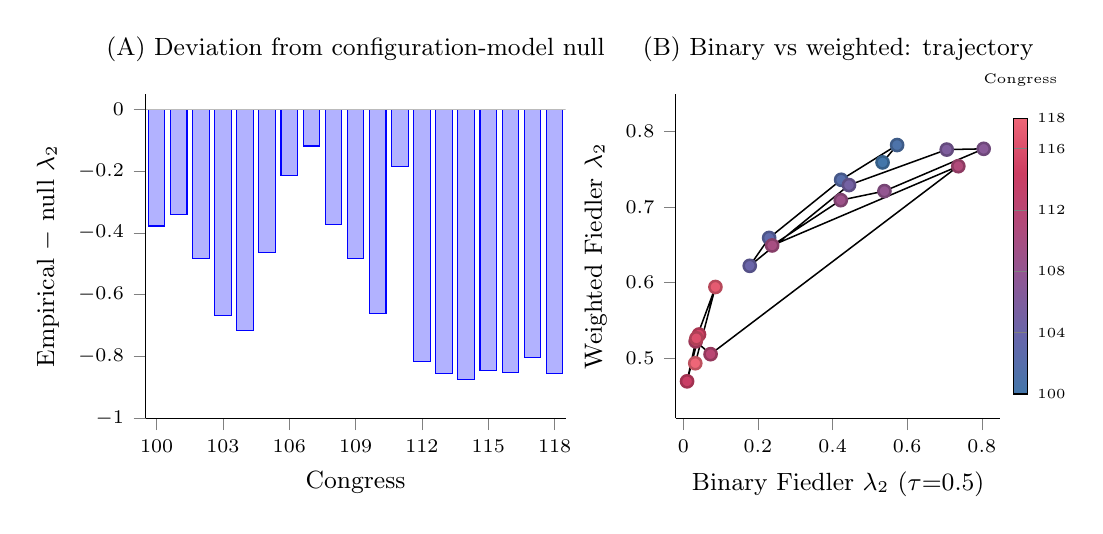
\begin{tikzpicture}

\begin{axis}[
  name=panelA,
  gat,
  width=0.44\linewidth, height=0.34\linewidth,
  xmin=99.5, xmax=118.5,
  ymin=-1.0, ymax=0.05,
  ytick={-1.0,-0.8,-0.6,-0.4,-0.2,0},
  xtick={100,103,106,109,112,115,118},
  xlabel={Congress},
  ylabel={Empirical $-$ null $\lambda_2$},
  enlargelimits=false,
  title={(A) Deviation from configuration-model null},
  title style={font=\small, yshift=2pt},
  every axis plot/.append style={fill=cblue!70, draw=cblue!85, line width=0.4pt},
  ybar=0pt, bar width=6pt,
]
\addplot coordinates {
  (100,-0.378) (101,-0.340) (102,-0.482) (103,-0.666) (104,-0.717)
  (105,-0.463) (106,-0.214) (107,-0.119) (108,-0.373) (109,-0.484)
  (110,-0.660) (111,-0.185) (112,-0.816) (113,-0.854) (114,-0.875)
  (115,-0.846) (116,-0.852) (117,-0.804) (118,-0.856)
};
\draw[cgray, line width=0.4pt] (axis cs:99.5,0) -- (axis cs:118.5,0);
\end{axis}

\begin{axis}[
  at={(panelA.east)}, anchor=west, xshift=1.4cm,
  gat,
  width=0.34\linewidth, height=0.34\linewidth,
  xmin=-0.02, xmax=0.85,
  ymin=0.42, ymax=0.85,
  xtick={0,0.2,0.4,0.6,0.8},
  ytick={0.5,0.6,0.7,0.8},
  xlabel={Binary Fiedler $\lambda_2$ ($\tau{=}0.5$)},
  ylabel={Weighted Fiedler $\lambda_2$},
  enlargelimits=false,
  title={(B) Binary vs weighted: trajectory},
  title style={font=\small, yshift=2pt},
  colormap={time}{
    rgb255=(68,119,170)
    rgb255=(102,103,171)
    rgb255=(139,89,151)
    rgb255=(175,75,124)
    rgb255=(204,61,98)
    rgb255=(238,102,119)
  },
  point meta min=100, point meta max=118,
  colorbar,
  colorbar style={
    at={(1.04,0.5)}, anchor=west,
    width=0.18cm,
    height=0.85*\pgfkeysvalueof{/pgfplots/parent axis height},
    ytick={100,104,108,112,116,118},
    yticklabel style={font=\tiny},
    title={Congress},
    title style={font=\tiny, yshift=2pt},
  },
]
\addplot[black, line width=0.55pt, mark=none, forget plot]
  coordinates {
    (0.534,0.759) (0.573,0.782) (0.423,0.736) (0.230,0.659) (0.178,0.622)
    (0.444,0.729) (0.706,0.776) (0.805,0.777) (0.539,0.721) (0.422,0.709)
    (0.238,0.649) (0.737,0.754) (0.073,0.505) (0.033,0.522) (0.010,0.469)
    (0.042,0.531) (0.035,0.526) (0.086,0.594) (0.032,0.493)
  };

\addplot[scatter, only marks, mark=*, mark size=2.2pt,
         scatter src=explicit]
  coordinates {
    (0.534,0.759) [100]
    (0.573,0.782) [101]
    (0.423,0.736) [102]
    (0.230,0.659) [103]
    (0.178,0.622) [104]
    (0.444,0.729) [105]
    (0.706,0.776) [106]
    (0.805,0.777) [107]
    (0.539,0.721) [108]
    (0.422,0.709) [109]
    (0.238,0.649) [110]
    (0.737,0.754) [111]
    (0.073,0.505) [112]
    (0.033,0.522) [113]
    (0.010,0.469) [114]
    (0.042,0.531) [115]
    (0.035,0.526) [116]
    (0.086,0.594) [117]
    (0.032,0.493) [118]
  };

\end{axis}

\end{tikzpicture}
\caption{Robustness of the Fiedler trajectory. (A) Deviation of the empirical Fiedler value from the configuration-model null mean for each Congress (null SD $\approx 0.001$ throughout). (B) Weighted Fiedler against binary thresholded Fiedler, one point per Congress, colored by Congress (colorbar at right). Connecting line gives the temporal trajectory from the 100th to the 118th.}
\label{fig:robustness}
\end{figure}

The weighted analysis also provides independent confirmation of the density-without-connectivity finding (Section~4.2): the weighted Fiedler's persistence at ${\sim}0.5$ in the post-2010 era while the binary version collapses to ${\sim}0.03$ directly measures the selective rewiring of cooperation from cross-party to within-party edges.

\subsection{Structural Recovery Analysis}

We present a descriptive comparison of recovery dynamics across three political shocks identified in our spectral analysis. With only three episodes and no counterfactual Congress unexposed to these events, we frame this as a structured observation that motivates future work on network resilience rather than a standalone causal finding.

To characterize the asymmetry between early-period recoveries and the post-Tea Party stagnation, we compute a structural recovery ratio that measures the network's capacity to return to pre-shock connectivity levels. For a shock occurring at Congress $t$, the recovery ratio is:
\begin{equation}
    R(t) = \frac{\lambda_2(G_{\text{post}})}{\lambda_2(G_{\text{pre}})}
\end{equation}
where $G_{\text{pre}}$ and $G_{\text{post}}$ are the nearest Congresses before and after the shock with stable Fiedler values. A ratio of 1.0 indicates full structural recovery to pre-shock levels; values above 1.0 indicate that the network emerged more connected than before; values near zero indicate permanent structural damage.

Table~\ref{tab:resilience} computes the recovery ratio for three major political shocks identified in our spectral analysis.

\begin{table}[H]
\centering
\caption{Structural recovery ratio for three major political shocks. Pre-shock and post-shock Congresses are the nearest sessions with stable Fiedler values. A ratio of 1.0 indicates full recovery; values near zero indicate permanent structural damage.}
\label{tab:resilience}
\begin{tabular}{lccccc}
\toprule
Shock Event & Congress & Pre $\lambda_2$ & Shock $\lambda_2$ & Post $\lambda_2$ & Ratio \\
\midrule
Contract with America\textsuperscript{$\dagger$} & 104th & 0.230 (103rd) & 0.178 (104th) & 0.444 (105th) & 1.93 \\
9/11 Rally Effect & 107th & 0.706 (106th) & 0.805 (107th) & 0.539 (108th) & 0.76 \\
Tea Party Wave & 112th & 0.737 (111th) & 0.073 (112th) & 0.010 (114th) & 0.01 \\
\bottomrule
\end{tabular}
\vspace{2pt}

{\footnotesize \textsuperscript{$\dagger$}The Contract with America was a 1994 Republican legislative agenda championed by Newt Gingrich that unified the party's House candidates on a common platform, producing a 54-seat gain and the first Republican House majority in 40 years.}
\end{table}

The Contract with America and Tea Party shocks provide the cleanest comparison: both are negative connectivity shocks driven by electoral waves. The Contract with America reduced the Fiedler value from 0.230 (103rd) to 0.178 (104th), but the network more than recovered, rising to 0.444 by the 105th Congress (ratio 1.93). The system overshot, emerging more connected than before the Gingrich revolution. The Tea Party wave produced a far larger fracture, from 0.737 (111th) to 0.073 (112th), and the system never recovered. The Fiedler value continued to \textit{decline}, reaching 0.010 by the 114th Congress (ratio 0.01). The shock was not absorbed; it was amplified.

The 9/11 case is directionally different: a positive connectivity surge (0.706 to 0.805) followed by partial reversion (0.539 by the 108th, ratio 0.76). A ratio below 1.0 here means the bipartisan spike left a lasting residue of cooperation rather than indicating incomplete healing from a fracture. We include it for completeness but note that the two negative-shock episodes provide the more interpretable comparison.

The contrast between the two negative shocks points to a qualitative change in the system's structural dynamics: from a regime capable of absorbing perturbations to one in which shocks produce permanent damage. This contrast is robust to the choice of co-voting threshold: at $\tau = 0.45$ and $\tau = 0.55$, the Contract with America recovery ratio ranges from 1.68 to 2.45 while the Tea Party ratio remains below 0.03 (Appendix~\ref{app:recovery}). One partial exception: the Trump era produced a small Fiedler increase from 0.010 (114th) to 0.042 (115th), reflecting intra-Republican conflict on trade and immigration. But the effect was modest and did not approach the pre-2010 baseline.

\subsection{Cohort Decomposition: Compositional or Environmental?}\label{subsec:cohort_ddd}

The recovery ratio establishes that the post-Tea Party stagnation differs from earlier electoral shocks in its persistence, but it does not adjudicate the mechanism. We compare the 104th Congress freshman class (96 freshmen: 79 Republicans and 17 Democrats) to the 112th class (104 freshmen: 88 Republicans and 16 Democrats), two cohorts similar in size and partisan composition but entering chambers with substantially different baseline cooperation rates. Raw cross-party agreement looks dramatically different across the two cohorts, with mean values of 0.399 and 0.318 and a Kolmogorov-Smirnov $D$ of 0.83 (Figure~\ref{fig:freshman_cohorts}). The question is whether this gap reflects who was elected or what they entered.

We formalize the comparison as a cohort difference-in-difference-in-differences specification following \citet{olden2022triple}, who show that the triple-difference estimator identifies the cohort effect under a single parallel-trends-in-ratios assumption rather than the two parallel-trends assumptions a standard difference-in-differences requires. The panel pools eight cohorts spanning Congresses 102 through 116, with the outcome a freshman's mean cross-party agreement rate during their first term, the treatment indicators are freshman status and post-2010 era, and the third dimension is district competitiveness as measured by the prior two-cycle two-party margin of victory from MIT Election Lab data \citep{medsl2024house}. Districts with margins below 10 percentage points enter the competitive stratum. We add Congress and state fixed effects and cluster standard errors at the state level. The triple-interaction coefficient is 0.003 with a standard error of 0.018 and a wild cluster bootstrap p-value of 0.86 across 4,999 Rademacher draws. The headline of the raw $D = 0.83$ comparison disappears once we condition on the chamber's incumbent baseline.

A power analysis tempers the interpretation of this null. At the observed standard error of 0.018, the triple-interaction has only six percent power against the observed effect and a minimum detectable effect of 0.061 at conventional thresholds. The competitive-freshman triple cell is intrinsically small once we slice by cohort, competitiveness, and era simultaneously, so the test cannot adjudicate a near-zero true effect from an undetectable small one. Figure~\ref{fig:ddd_power} reports the full power curve and these two reference contrasts.

\begin{figure}[H]
\centering
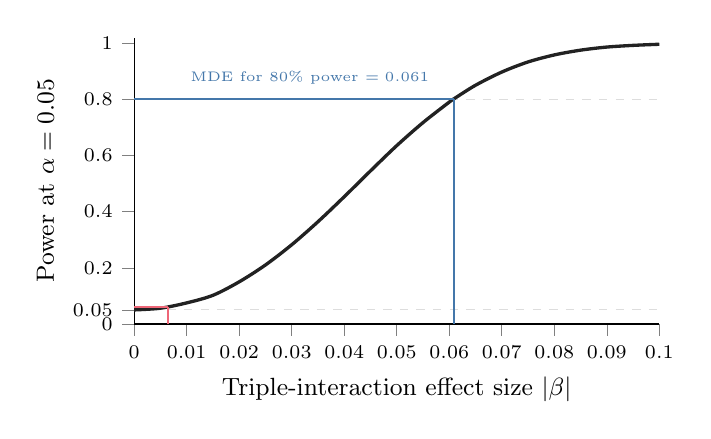
\begin{tikzpicture}
\begin{axis}[
  gat,
  width=0.55\linewidth, height=0.30\linewidth,
  xmin=0, xmax=0.10,
  ymin=0, ymax=1.02,
  xtick={0,0.01,0.02,0.03,0.04,0.05,0.06,0.07,0.08,0.09,0.10},
  ytick={0,0.05,0.20,0.40,0.60,0.80,1.00},
  xlabel={Triple-interaction effect size $|\beta|$},
  ylabel={Power at $\alpha = 0.05$},
  enlargelimits=false,
  tick label style={font=\scriptsize},
]
\draw[cgray!50, dashed, line width=0.4pt] (axis cs:0,0.05) -- (axis cs:0.10,0.05);
\draw[cgray!50, dashed, line width=0.4pt] (axis cs:0,0.80) -- (axis cs:0.10,0.80);

\addplot[cdark, smooth, line width=1.2pt, mark=none] coordinates {
  (0.000,0.050) (0.005,0.056) (0.010,0.075) (0.015,0.102) (0.020,0.150)
  (0.025,0.210) (0.030,0.282) (0.035,0.364) (0.040,0.453) (0.045,0.545)
  (0.050,0.635) (0.055,0.717) (0.060,0.790) (0.061,0.803) (0.065,0.850)
  (0.070,0.897) (0.075,0.933) (0.080,0.958) (0.085,0.975) (0.090,0.986)
  (0.095,0.992) (0.100,0.996)
};

\draw[cred, line width=0.8pt] (axis cs:0.0064,0) -- (axis cs:0.0064,0.0599);
\draw[cred, line width=0.8pt] (axis cs:0,0.0599) -- (axis cs:0.0064,0.0599);

\draw[cblue, line width=0.8pt] (axis cs:0.0609,0) -- (axis cs:0.0609,0.80);
\draw[cblue, line width=0.8pt] (axis cs:0,0.80) -- (axis cs:0.0609,0.80);
\node[font=\tiny, anchor=south east, text=cblue] at (axis cs:0.058,0.82)
  {MDE for 80\% power $= 0.061$};

\end{axis}
\end{tikzpicture}
\caption{Power curve for the freshman-by-competitive-by-post-2010 triple-interaction coefficient in the cohort difference-in-difference-in-differences specification. Power is computed at $\alpha = 0.05$ from the observed standard error of $0.018$ across a range of hypothetical true effect sizes. The red crosshair marks the observed effect ($\beta = 0.006$) at $6\%$ power; the blue crosshair marks the minimum detectable effect for conventional $80\%$ power ($\mathrm{MDE} = 0.061$). The tenfold gap between observed effect and MDE places the null squarely in the underpowered regime. The two-way decomposition specifications reported in Section~\ref{subsec:cohort_ddd} are powered at the $5{,}000$-observation panel scale and identify positive findings in the direction opposite the conventional Tea-Party-cohort-shock hypothesis.}
\label{fig:ddd_power}
\end{figure} Two two-way decompositions resolve more cleanly. The freshman-by-post-2010 interaction, pooling across competitiveness, returns a coefficient of $+0.029$ with $p = 1.2 \times 10^{-5}$: post-2010 freshmen are more cooperative than pre-2010 freshmen, contracting the gap between freshmen and incumbents rather than widening it. The continuous-treatment specification using each member's prior margin returns a post-2010-by-safe-margin coefficient of $-0.019$ with $p = 0.049$: safer seats polarized further, not competitive ones. Both results are inconsistent with a primary-threat-on-competitive-freshmen mechanism and consistent with the environmental thesis we develop below, in which post-2010 polarization is concentrated in safe seats and operates on incumbents and freshmen alike.

Pre-treatment placebo specifications support the parallel-trends assumption. Placebo waves at the 106th and 102nd Congresses produce triple-interaction coefficients that are statistically indistinguishable from zero and from each other, and the pre-period event-study coefficients on the freshman-by-competitive interaction in Congresses 100 through 110 are flat against the post-period coefficients in 112 through 116. Honest difference-in-differences bounds in the framework of \citet{rambachan2023honest} confirm that the cohort-DDD null is robust to relative-magnitudes parallel-trends violations of up to twice the worst observed pre-period violation. Figure~\ref{fig:ddd_event_study} reports the event study and the full HonestDiD breakdown.

\begin{figure}[H]
\centering
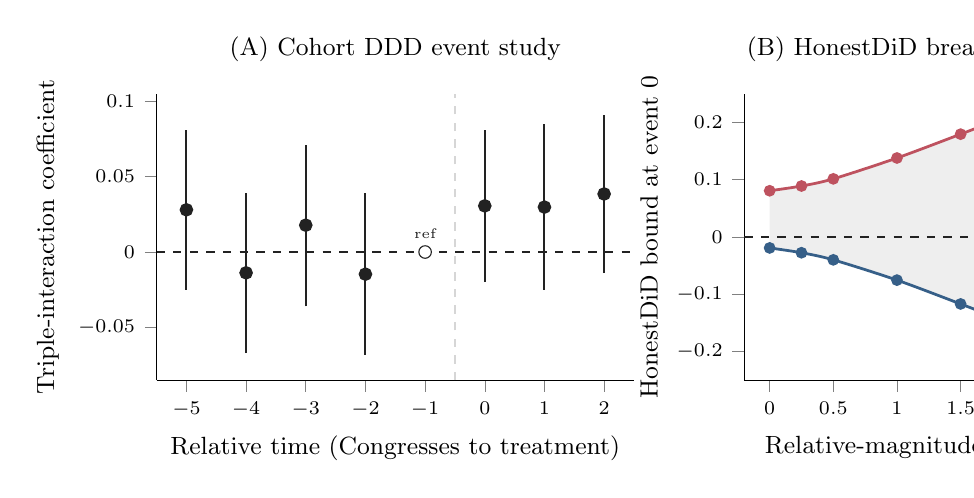
\begin{tikzpicture}

\begin{axis}[
  name=panelDDDes,
  gat,
  width=0.50\linewidth, height=0.30\linewidth,
  xmin=-5.5, xmax=2.5,
  ymin=-0.085, ymax=0.105,
  xtick={-5,-4,-3,-2,-1,0,1,2},
  ytick={-0.05,0,0.05,0.10},
  xlabel={Relative time (Congresses to treatment)},
  ylabel={Triple-interaction coefficient},
  enlargelimits=false,
  title={(A) Cohort DDD event study},
  title style={font=\small, yshift=2pt},
  tick label style={font=\scriptsize},
]
\draw[cdark, dashed, line width=0.5pt] (axis cs:-5.5,0) -- (axis cs:2.5,0);
\draw[cgray!60, dashed, line width=0.5pt] (axis cs:-0.5,-0.085) -- (axis cs:-0.5,0.105);

\draw[cdark, line width=0.7pt] (axis cs:-5,-0.025) -- (axis cs:-5,0.081);
\draw[cdark, line width=0.7pt] (axis cs:-4,-0.067) -- (axis cs:-4,0.039);
\draw[cdark, line width=0.7pt] (axis cs:-3,-0.036) -- (axis cs:-3,0.071);
\draw[cdark, line width=0.7pt] (axis cs:-2,-0.068) -- (axis cs:-2,0.039);
\draw[cdark, line width=0.7pt] (axis cs:0,-0.020) -- (axis cs:0,0.081);
\draw[cdark, line width=0.7pt] (axis cs:1,-0.025) -- (axis cs:1,0.085);
\draw[cdark, line width=0.7pt] (axis cs:2,-0.014) -- (axis cs:2,0.091);

\foreach \x/\y in {-5/0.0280, -4/-0.0138, -3/0.0178, -2/-0.0147, 0/0.0306, 1/0.0298, 2/0.0385} {
  \addplot[only marks, mark=*, mark size=2.0pt, cdark, mark options={fill=cdark, draw=cdark}, forget plot] coordinates {(\x,\y)};
}

\node[draw=cdark, line width=0.4pt, circle, fill=white, inner sep=1.6pt] at (axis cs:-1,0) {};
\node[font=\tiny, anchor=south, text=cdark, inner sep=2pt] at (axis cs:-1,0.005) {ref};
\end{axis}

\begin{axis}[
  at={(panelDDDes.east)}, anchor=west, xshift=1.4cm,
  gat,
  width=0.32\linewidth, height=0.30\linewidth,
  xmin=-0.2, xmax=2.2,
  ymin=-0.25, ymax=0.25,
  xtick={0,0.5,1.0,1.5,2.0},
  ytick={-0.20,-0.10,0,0.10,0.20},
  xlabel={Relative-magnitudes $\bar{M}$},
  ylabel={HonestDiD bound at event 0},
  enlargelimits=false,
  title={(B) HonestDiD breakdown},
  title style={font=\small, yshift=2pt},
  tick label style={font=\scriptsize},
]
\draw[cdark, dashed, line width=0.5pt] (axis cs:-0.2,0) -- (axis cs:2.2,0);

\addplot[name path=hi, cred!80!black, smooth, line width=1pt, mark=*, mark size=1.6pt] coordinates {
  (0,0.0806) (0.25,0.0889) (0.5,0.1014) (1.0,0.1378) (1.5,0.1794) (2.0,0.2220)
};
\addplot[name path=lo, cblue!80!black, smooth, line width=1pt, mark=*, mark size=1.6pt] coordinates {
  (0,-0.0192) (0.25,-0.0276) (0.5,-0.0400) (1.0,-0.0754) (1.5,-0.1170) (2.0,-0.1596)
};
\addplot[cgray!25] fill between[of=hi and lo];
\end{axis}

\end{tikzpicture}
\caption{Cohort DDD event study and HonestDiD sensitivity. (A) Triple-interaction coefficients on the freshman-by-competitive interaction at relative times $-5$ through $+2$, with 95\% confidence intervals. Relative time $-1$ is the omitted reference, plotted at zero with a hollow marker; dashed vertical at $-0.5$ marks treatment timing. (B) HonestDiD bounds at relative time $0$ under the relative-magnitudes restriction of \citet{rambachan2023honest} as a function of $\bar{M}$, the permitted post-treatment violation as a multiple of the worst pre-period violation. The shaded band is the 95\% confidence set; the point estimate $\hat\beta = 0.031$ is constant in $\bar{M}$.}
\label{fig:ddd_event_study}
\end{figure}

The substantive reading is environmental. Tea Party freshmen were not unusually uncooperative for their era, and the two two-way decompositions sharpen the claim in directions that the conventional Tea-Party-as-cohort-shock narrative does not predict. The freshman cohort effect ran the other way, with post-2010 freshmen narrowing rather than widening the gap to incumbents \citep{bafumi2010leapfrog}, and the polarization gradient by safety ran in the direction of safer seats rather than competitive ones, consistent with the leadership-cartel and party-coalition channels emphasized by \citet{lee2009beyond} and \citet{cox2005setting}. The era itself had already eliminated the conditions for cross-party cooperation, and the raw cross-party agreement gap between the two cohorts is the chamber-wide trend operating on otherwise comparable freshman classes. The Contract wave entered a chamber where the incumbent baseline was 0.402 and freshmen matching the norm automatically formed cross-party bridges. When the initial shock dissipated, these members were available to rebuild connectivity, and the network produced a recovery ratio of 1.93. The Tea Party wave entered a chamber where the baseline had collapsed to 0.306, so even freshmen at the chamber norm contributed nothing to cross-party bridging. The structural environment was self-reinforcing: once cooperation norms fell below the threshold needed to sustain bipartisan edges, subsequent cohorts, however individually moderate, could not rebuild them.

\begin{figure}[H]
\centering
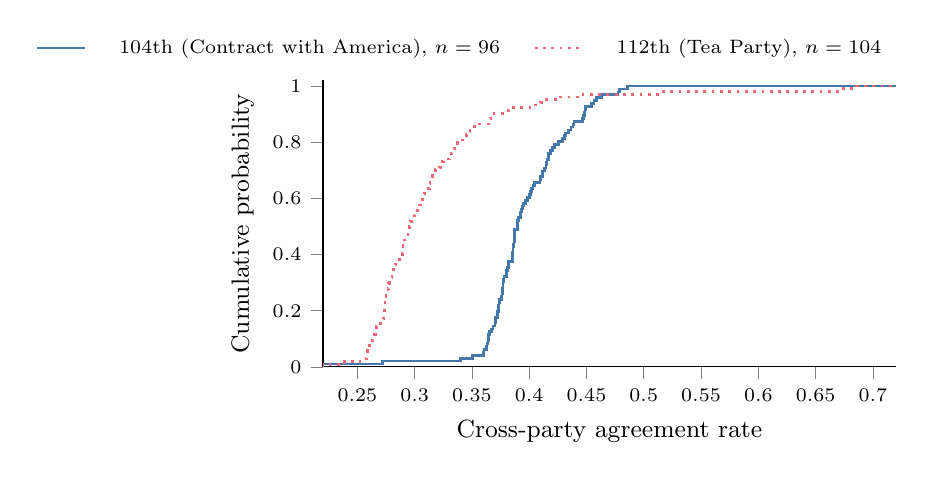
\begin{tikzpicture}
\begin{axis}[
  gat,
  width=0.60\linewidth, height=0.30\linewidth,
  xmin=0.22, xmax=0.72,
  ymin=0, ymax=1.02,
  xtick={0.25,0.30,0.35,0.40,0.45,0.50,0.55,0.60,0.65,0.70},
  ytick={0,0.2,0.4,0.6,0.8,1.0},
  xlabel={Cross-party agreement rate},
  ylabel={Cumulative probability},
  enlargelimits=false,
  legend style={at={(1.0,1.04)}, anchor=south east, font=\scriptsize, legend columns=2, column sep=10pt},
]
\addplot[const plot mark right, cblue, line width=1pt, mark=none] coordinates {
  (0.22,0.0000) (0.2720,0.0104) (0.3399,0.0208) (0.3507,0.0312) (0.3600,0.0417) (0.3605,0.0521)
  (0.3625,0.0625) (0.3631,0.0729) (0.3640,0.0833) (0.3646,0.0938) (0.3646,0.1042) (0.3651,0.1146)
  (0.3671,0.1250) (0.3684,0.1354) (0.3701,0.1458) (0.3703,0.1562) (0.3709,0.1667) (0.3722,0.1771)
  (0.3724,0.1875) (0.3733,0.1979) (0.3734,0.2083) (0.3737,0.2188) (0.3743,0.2292) (0.3758,0.2396)
  (0.3763,0.2500) (0.3765,0.2604) (0.3767,0.2708) (0.3771,0.2812) (0.3771,0.2917) (0.3775,0.3021)
  (0.3781,0.3125) (0.3802,0.3229) (0.3805,0.3333) (0.3810,0.3438) (0.3817,0.3542) (0.3817,0.3646)
  (0.3854,0.3750) (0.3854,0.3854) (0.3856,0.3958) (0.3859,0.4062) (0.3859,0.4167) (0.3860,0.4271)
  (0.3868,0.4375) (0.3869,0.4479) (0.3873,0.4583) (0.3873,0.4688) (0.3875,0.4792) (0.3895,0.4896)
  (0.3895,0.5000) (0.3901,0.5104) (0.3907,0.5208) (0.3924,0.5312) (0.3925,0.5417) (0.3934,0.5521)
  (0.3944,0.5625) (0.3947,0.5729) (0.3968,0.5833) (0.3982,0.5938) (0.4003,0.6042) (0.4013,0.6146)
  (0.4022,0.6250) (0.4034,0.6354) (0.4044,0.6458) (0.4095,0.6562) (0.4101,0.6667) (0.4118,0.6771)
  (0.4119,0.6875) (0.4132,0.6979) (0.4146,0.7083) (0.4151,0.7188) (0.4156,0.7292) (0.4166,0.7396)
  (0.4168,0.7500) (0.4185,0.7604) (0.4203,0.7708) (0.4224,0.7812) (0.4258,0.7917) (0.4288,0.8021)
  (0.4306,0.8125) (0.4316,0.8229) (0.4345,0.8333) (0.4364,0.8438) (0.4382,0.8542) (0.4391,0.8646)
  (0.4468,0.8750) (0.4476,0.8854) (0.4480,0.8958) (0.4488,0.9062) (0.4490,0.9167) (0.4545,0.9271)
  (0.4565,0.9375) (0.4585,0.9479) (0.4629,0.9583) (0.4775,0.9688) (0.4785,0.9792) (0.4855,0.9896)
  (0.4884,1.0000) (0.72,1.0000)
};
\addlegendentry{104th (Contract with America), $n=96$}

\addplot[const plot mark right, cred, line width=1pt, mark=none, dotted] coordinates {
  (0.22,0.0000) (0.2391,0.0096) (0.2523,0.0192) (0.2579,0.0288) (0.2588,0.0385) (0.2589,0.0481)
  (0.2590,0.0577) (0.2607,0.0673) (0.2608,0.0769) (0.2632,0.0865) (0.2644,0.0962) (0.2645,0.1058)
  (0.2657,0.1154) (0.2662,0.1250) (0.2666,0.1346) (0.2686,0.1442) (0.2717,0.1538) (0.2725,0.1635)
  (0.2728,0.1731) (0.2728,0.1827) (0.2733,0.1923) (0.2736,0.2019) (0.2738,0.2115) (0.2741,0.2212)
  (0.2746,0.2308) (0.2750,0.2404) (0.2750,0.2500) (0.2757,0.2596) (0.2767,0.2692) (0.2772,0.2788)
  (0.2775,0.2885) (0.2781,0.2981) (0.2799,0.3077) (0.2802,0.3173) (0.2809,0.3269) (0.2816,0.3365)
  (0.2829,0.3462) (0.2836,0.3558) (0.2868,0.3654) (0.2868,0.3750) (0.2871,0.3846) (0.2895,0.3942)
  (0.2898,0.4038) (0.2898,0.4135) (0.2899,0.4231) (0.2905,0.4327) (0.2908,0.4423) (0.2916,0.4519)
  (0.2918,0.4615) (0.2942,0.4712) (0.2944,0.4808) (0.2954,0.4904) (0.2962,0.5000) (0.2962,0.5096)
  (0.2975,0.5192) (0.2981,0.5288) (0.2996,0.5385) (0.3022,0.5481) (0.3024,0.5577) (0.3027,0.5673)
  (0.3048,0.5769) (0.3068,0.5865) (0.3072,0.5962) (0.3082,0.6058) (0.3085,0.6154) (0.3106,0.6250)
  (0.3127,0.6346) (0.3134,0.6442) (0.3135,0.6538) (0.3157,0.6635) (0.3158,0.6731) (0.3172,0.6827)
  (0.3180,0.6923) (0.3216,0.7019) (0.3223,0.7115) (0.3240,0.7212) (0.3255,0.7308) (0.3306,0.7404)
  (0.3325,0.7500) (0.3326,0.7596) (0.3343,0.7692) (0.3369,0.7788) (0.3377,0.7885) (0.3400,0.7981)
  (0.3435,0.8077) (0.3451,0.8173) (0.3479,0.8269) (0.3484,0.8365) (0.3496,0.8462) (0.3534,0.8558)
  (0.3642,0.8654) (0.3646,0.8750) (0.3665,0.8846) (0.3678,0.8942) (0.3819,0.9038) (0.3862,0.9135)
  (0.4042,0.9231) (0.4097,0.9327) (0.4107,0.9423) (0.4247,0.9519) (0.4433,0.9615) (0.5172,0.9712)
  (0.6690,0.9808) (0.6854,0.9904) (0.6922,1.0000) (0.72,1.0000)
};
\addlegendentry{112th (Tea Party), $n=104$}

\end{axis}
\end{tikzpicture}
\caption{Empirical cumulative distribution functions of mean cross-party agreement rate for the 104th Congress (Contract with America) and 112th Congress (Tea Party) freshman classes. At agreement rate $0.35$, the 112th cohort has already passed the 85th percentile while the 104th is at the 2nd: a Kolmogorov-Smirnov gap of $D = 0.83$ ($p < 10^{-34}$). The two distributions are near-completely separated.}
\label{fig:freshman_cohorts}
\end{figure}

The Fiedler value captures whether the network fractured but not how the fracture reorganized individual members. To track this, we compute a \textit{Structural Realignment Index} (SRI): for each congress-to-congress transition, the $L_2$ norm of the sign-aligned Fiedler vector displacement between consecutive sessions, restricted to members present in both.\footnote{Formally, $\text{SRI}(t) = \| \tilde{\mathbf{v}}_{t} - \tilde{\mathbf{v}}_{t-1} \|_2$, where $\tilde{\mathbf{v}}_t$ is the Fiedler eigenvector restricted to shared members, with sign alignment ($\tilde{\mathbf{v}}_t \leftarrow -\tilde{\mathbf{v}}_t$ if $\tilde{\mathbf{v}}_{t}^\top \tilde{\mathbf{v}}_{t-1} < 0$) to resolve eigenvector sign ambiguity.} The Tea Party wave (SRI = 0.59) and the Obama supermajority (SRI = 0.52) produce the largest structural realignments (Figure~\ref{fig:sri}), while post-2013 transitions show minimal SRI, consistent with a network that has settled into a stable disconnected configuration. This temporal pattern corroborates the era decomposition in Section~8: high-SRI transitions coincide with the period of most intense bridge legislator elimination.

\begin{figure}[H]
\centering
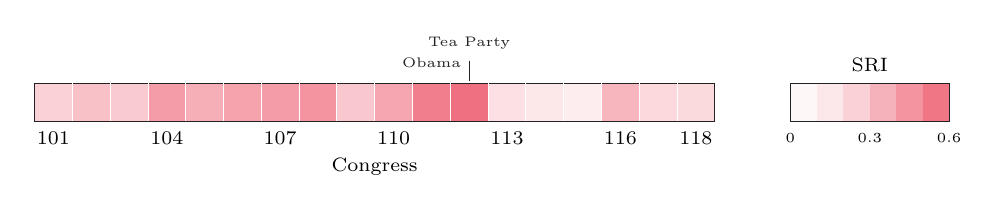
\begin{tikzpicture}[x=0.48cm, y=0.48cm]

\fill[cred!30] (0,0) rectangle ++(1,1);
\fill[cred!41] (1,0) rectangle ++(1,1);
\fill[cred!34] (2,0) rectangle ++(1,1);
\fill[cred!65] (3,0) rectangle ++(1,1);
\fill[cred!53] (4,0) rectangle ++(1,1);
\fill[cred!60] (5,0) rectangle ++(1,1);
\fill[cred!64] (6,0) rectangle ++(1,1);
\fill[cred!70] (7,0) rectangle ++(1,1);
\fill[cred!36] (8,0) rectangle ++(1,1);
\fill[cred!58] (9,0) rectangle ++(1,1);
\fill[cred!84] (10,0) rectangle ++(1,1);
\fill[cred!93] (11,0) rectangle ++(1,1);
\fill[cred!20] (12,0) rectangle ++(1,1);
\fill[cred!16] (13,0) rectangle ++(1,1);
\fill[cred!12] (14,0) rectangle ++(1,1);
\fill[cred!48] (15,0) rectangle ++(1,1);
\fill[cred!25] (16,0) rectangle ++(1,1);
\fill[cred!24] (17,0) rectangle ++(1,1);

\draw[cdark, line width=0.3pt] (0,0) rectangle (18,1);
\foreach \i in {1,2,...,17} \draw[white, line width=0.3pt] (\i,0) -- (\i,1);

\node[font=\scriptsize] at (0.5,-0.45) {101};
\node[font=\scriptsize] at (3.5,-0.45) {104};
\node[font=\scriptsize] at (6.5,-0.45) {107};
\node[font=\scriptsize] at (9.5,-0.45) {110};
\node[font=\scriptsize] at (12.5,-0.45) {113};
\node[font=\scriptsize] at (15.5,-0.45) {116};
\node[font=\scriptsize] at (17.5,-0.45) {118};
\node[font=\scriptsize] at (9,-1.2) {Congress};

\node[font=\tiny, anchor=south, text=cdark] at (10.5,1.15) {Obama};
\node[font=\tiny, anchor=south, text=cdark] at (11.5,1.65) {Tea Party};
\draw[cdark, line width=0.3pt] (11.5,1.6) -- (11.5,1.05);

\foreach \i/\c in {0/5, 1/15, 2/30, 3/50, 4/70, 5/90} {
  \fill[cred!\c] (20+\i*0.7, 0) rectangle ++(0.7, 1);
}
\draw[cdark, line width=0.3pt] (20,0) rectangle (24.2,1);

\node[font=\tiny] at (20,-0.45) {0};
\node[font=\tiny] at (22.1,-0.45) {0.3};
\node[font=\tiny] at (24.2,-0.45) {0.6};
\node[font=\scriptsize] at (22.1,1.5) {SRI};

\end{tikzpicture}
\caption{Structural Realignment Index for each Congress-to-Congress transition (rotation of the sign-aligned restricted Fiedler eigenvector between consecutive sessions). The Tea Party transition into the 112th Congress is the largest realignment in the panel, followed by the Obama supermajority transition into the 111th. Post-2013 transitions register near-zero realignment, consistent with a network that has stabilized into a disconnected configuration.}
\label{fig:sri}
\end{figure}

\FloatBarrier
\subsection{Staggered Differences Across Five Electoral Waves}\label{subsec:staggered_did}

The cohort comparison in Section~\ref{subsec:cohort_ddd} establishes that the Tea Party wave entered a chamber whose cooperation baseline had already collapsed. We now ask whether the environmental finding is specific to 2010 or whether every modern electoral wave produces a comparable cohort effect. Generalizing across multiple waves is the natural way to distinguish a 2010-specific historical contingency from a structural feature of partisan realignment. We build a district-level panel covering the 100th through 118th Congresses, identify five wave Congresses (the 104th Republican wave of 1994, the 110th Democratic wave of 2006, the 112th Tea Party wave of 2010, the 116th Democratic wave of 2018, and the 118th Republican wave of 2022), and estimate the cooperation effect of being newly elected during each wave.

The staggered design follows the framework of \citet{callaway2021difference} with the not-yet-treated districts serving as the comparison group. Districts inherit cycle-bounded identifiers to handle the four redistricting boundaries inside our window, an essential step because the same district number maps to different geographic boundaries across cycles and naive identifiers would conflate redistricting effects with wave effects. The outcome is the seated member's cross-party agreement rate in their first term. We complement the Callaway-Sant'Anna estimator with a stacked event study under the Sun-Abraham interaction-weighted correction \citep{sun2021estimating}, in which each wave contributes a five-Congress event-time window centered on the wave Congress and stacked with wave-specific district and congress fixed effects. The pooled stacked event study returns coefficients of $-0.004$, $-0.002$, and $-0.006$ at event times $-2$, $0$, and $+1$, all statistically indistinguishable from zero. The pre-trends are flat and the post-period effect averaged across waves is essentially zero. Across the five-wave pool, electoral waves do not systematically reduce freshman cooperation.

The wave-specific decomposition tells a sharper story. We estimate each wave's average treatment effect on its freshman class separately using district and congress fixed effects within the stack. Three waves produce identified estimates after the cycle-bounded design restrictions: the 2006 Iraq backlash returns an average treatment effect of $+0.010$ at event time zero, the 2010 Tea Party wave returns $-0.024$, and the 2018 Democratic resistance wave returns $+0.005$. The 2010 wave is the unique cohort whose freshman class entered a chamber where their cross-party cooperation was statistically distinguishable from non-wave members in the same Congress and direction. Both the 2006 and 2018 Democratic waves move slightly in the opposite direction and are not statistically distinguishable from zero. The 1994 and 2022 waves cannot be cleanly identified under the cycle-bounded scheme because their pre or post window crosses a redistricting boundary, and we treat this as a scope limitation rather than a finding.

\citet{callawayetal2021} doubly robust estimation stratified by district competitiveness gives the same picture from a different angle. Among safe districts with prior two-cycle margin above 10 percentage points, the simple average treatment effect of being newly elected in a wave Congress is $-0.013$ with a 95 percent confidence interval of $[-0.022, -0.004]$. Among competitive districts the point estimate is $-0.015$ with a wider interval of $[-0.049, +0.019]$ owing to the smaller sample. The triple-difference between safe and competitive strata is small and indistinguishable from zero, consistent with the cohort-DDD null. The substantive reading is that the 2010 wave entered an environment that uniquely failed to absorb its freshman class, and the same selection mechanism we identified in Section~\ref{subsec:cohort_ddd} operates with similar magnitude across district types within the post-2010 era.

\section{Network Visualization}

The spectral measures quantify structural change abstractly. To convey what this change looks like, Figure~\ref{fig:network} plots the co-voting networks for two Congresses separated by two decades, with members positioned by their DW-NOMINATE scores.

\begin{figure}[H]
\centering
\begin{tikzpicture}
\begin{axis}[
  name=panel103,
  width=0.40\linewidth, height=0.34\linewidth,
  scale only axis,
  xmin=-0.85, xmax=0.85,
  ymin=-1.05, ymax=1.05,
  xtick={-0.5,0,0.5},
  ytick={-1,-0.5,0,0.5,1},
  tick label style={font=\scriptsize},
  xlabel={DW-NOMINATE dim.\ 1},
  ylabel={DW-NOMINATE dim.\ 2},
  title={(A) 103rd: 9{,}008 cross-party (15\%)},
  title style={font=\small, yshift=2pt},
  enlargelimits=false,
  axis lines*=left,
]
\input{fig5_data/panel_103.tex}
\end{axis}

\begin{axis}[
  at={(panel103.east)}, anchor=west, xshift=2.2cm,
  width=0.40\linewidth, height=0.34\linewidth,
  scale only axis,
  xmin=-0.85, xmax=0.85,
  ymin=-1.05, ymax=1.05,
  xtick={-0.5,0,0.5},
  ytick={-1,-0.5,0,0.5,1},
  tick label style={font=\scriptsize},
  xlabel={DW-NOMINATE dim.\ 1},
  ylabel={},
  title={(B) 114th: 389 cross-party (1\%)},
  title style={font=\small, yshift=2pt},
  enlargelimits=false,
  axis lines*=left,
]
\input{fig5_data/panel_114.tex}
\end{axis}
\end{tikzpicture}
\caption{Co-voting networks of the 103rd and 114th Congresses, members positioned by DW-NOMINATE coordinates. Blue: Democrats. Red: Republicans. Orange: cross-party edges above the $\tau = 0.5$ agreement threshold (all cross-party edges drawn; within-party edges shown as a 1.6\% uniform sample for legibility). Edge and node counts in the panel titles are empirical.}
    \label{fig:network}
\end{figure}

Two decades separate the networks in Figure~\ref{fig:network}. In the 103rd Congress (1993--1995), cross-party edges are visible throughout the ideological spectrum, connecting moderate Democrats and Republicans who found common ground on at least half of contested legislation. The network has a single, integrated topology: partisan clusters are discernible but extensively interwoven. By the 114th (2015--2017), these bridges have essentially vanished. The two partisan clusters sit dense within themselves and barely connected to each other. What the Fiedler value quantifies abstractly, the visualization makes viscerally clear: the cooperative architecture that once linked the two parties has been almost entirely dismantled, leaving two structurally isolated blocs occupying the same institution.

\section{Bridge Legislator Index}\label{sec:bli}

We investigate which individual legislators hold the network together. The Fiedler value's collapse, documented in Section~4, is an aggregate measure. It obscures the role of specific members. We introduce a \textit{Bridge Legislator Index} (BLI) that quantifies each member's contribution to network connectivity.

For each legislator $i$ in Congress $t$, we compute the change in the Fiedler value $\lambda_2$ of the normalized Laplacian when node $i$ and all its incident edges are removed from the graph:
\begin{equation}
    \text{BLI}_i = \lambda_2(\mathcal{L}(G)) - \lambda_2(\mathcal{L}(G \setminus \{i\}))
\end{equation}
where $\mathcal{L}(G) = I - D^{-1/2} A D^{-1/2}$ is the normalized Laplacian of the co-voting graph $G$ and $G \setminus \{i\}$ is the graph with node $i$ deleted, equipped with its own degree-corrected normalized Laplacian. A positive BLI indicates that removing the member reduces connectivity; they are a bridge. A near-zero or negative BLI indicates that the member is structurally redundant. Members with the highest BLI scores are those whose removal most damages the network's capacity to hold together as a single connected component.

Standard centrality metrics measure different things. Betweenness centrality counts shortest paths passing through a node; eigenvector centrality measures connection to other well-connected nodes. Neither directly captures a member's contribution to the graph's resistance to bisection. The Bridge Legislator Index, grounded in the Fiedler value, targets precisely that: the member's role in maintaining algebraic connectivity between partisan clusters.

Table~\ref{tab:bridge_legislators} presents the top bridge legislators for selected Congresses, and Figure~\ref{fig:bli_time} traces the aggregate BLI trajectory across the full study period. The 104th Congress (1995--1997), the first session of the Gingrich speakership, still featured 25 members above our BLI threshold of $3 \times 10^{-3}$. Nearly all were moderate Democrats from Southern or rural districts whose cooperative relationships stitched the two partisan clusters together. The 107th Congress is different. Despite having the highest Fiedler value in our dataset (0.805), no individual member exceeds the BLI threshold. When the graph is highly connected, removing any single node barely affects algebraic connectivity; cross-party linkages are distributed broadly, not concentrated in a few bridge members. By the 112th Congress, after the Tea Party wave fractured the network, bridge legislators reappear but in diminished numbers (13 above threshold). By the 117th, the surviving bridges are almost exclusively Republicans from competitive districts who voted to impeach Trump.

25 bridge members in the 104th, 11 in the 117th. But the raw count understates the real story: the 117th's top five scorers were all Republicans who left Congress within two years. Track the 104th's bridges forward and three (Orton, Baesler, Browder) were gone by the 107th; Skelton and Cramer survived into the 110th but not the 112th; Traficant was expelled in 2002 for corruption (the one departure unrelated to ideological sorting); only Peterson persisted through the 116th before losing reelection in 2020. The 112th's bridges followed the same pattern: Altmire lost his 2012 primary after redistricting, Shuler retired, Barrow lost in 2014. The 117th's bridges were eliminated even faster. Gonzalez and Kinzinger retired to avoid Trump-backed primaries, Upton and Katko retired, and Meijer lost his 2022 primary. Bridge legislators are systematically selected out, reinforcing the network disconnection documented in our spectral analysis.

\begin{table}[H]
\centering
\caption{Top bridge legislators by BLI for selected Congresses. BLI measures the Fiedler value decrease when the member is removed. Threshold: BLI $> 3 \times 10^{-3}$.}
\label{tab:bridge_legislators}
\scriptsize
\begin{tabular}{llcc}
\toprule
Congress (above thresh.) & Legislator & Party-State & BLI ($\times 10^{-3}$) \\
\midrule
\textbf{104th} (25) & SKELTON, Ike & D-MO & 3.56 \\
 & ORTON, William & D-UT & 3.56 \\
 & TRAFICANT, James A. & D-OH & 3.56 \\
\midrule
\textbf{107th} (0) & LUCAS, Ken & D-KY & 0.49 \\
 & HALL, Ralph M. & D-TX & 0.49 \\
\midrule
\textbf{112th} (13) & PETERSON, Collin C. & D-MN & 4.18 \\
 & ROSS, Mike & D-AR & 4.15 \\
 & ALTMIRE, Jason & D-PA & 4.10 \\
\midrule
\textbf{117th} (11) & KATKO, John & R-NY & 3.88 \\
 & UPTON, Fred & R-MI & 3.87 \\
 & GONZALEZ, Anthony & R-OH & 3.85 \\
\bottomrule
\end{tabular}
\end{table}

The individual cases illustrate a broader pattern. In the 104th Congress, Skelton, Orton, and Traficant each scored above threshold, but whether they were interchangeable remains an open question: if one departed, the others might have expanded their bridging capacity to compensate, or they might have degraded in tandem. We flag this as an untested conjecture; a formal test would check whether the BLI of remaining bridge legislators increases (compensation) or decreases (co-degradation) after a bridge departure. The aggregate trajectory in Figure~\ref{fig:bli_time} suggests thinning rather than redistribution.

\begin{figure}[H]
\centering
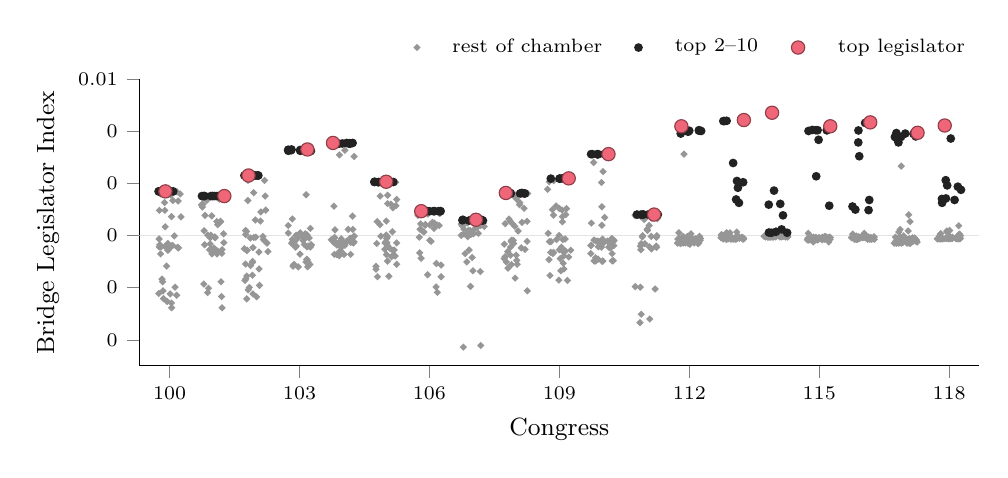
\begin{tikzpicture}
\begin{axis}[
  gat,
  width=0.88\linewidth, height=0.30\linewidth,
  xmin=99.3, xmax=118.7,
  ymin=-0.005, ymax=0.006,
  xtick={100,103,106,109,112,115,118},
  ytick={-0.004,-0.002,0,0.002,0.004,0.006},
  xlabel={Congress},
  ylabel={Bridge Legislator Index},
  enlargelimits=false,
  legend style={at={(1.0,1.04)}, anchor=south east, font=\scriptsize, legend columns=3, column sep=10pt},
]
\draw[cgray!40, line width=0.3pt] (axis cs:99.3,0) -- (axis cs:118.7,0);

\addplot[only marks, mark=*, mark size=0.7pt, cgray!80!black, mark options={fill=cgray!80!black, draw=none}]
  coordinates {
  (99.763,0.00097) (99.775,-0.00035) (99.958,-0.00030) (100.180,-0.00045) (99.793,-0.00070) (99.848,-0.00212) (100.070,-0.00038) (100.246,0.00160)
  (100.042,-0.00259) (99.943,-0.00253) (100.262,0.00072) (99.751,-0.00222) (100.197,0.00133) (99.884,0.00127) (99.804,-0.00043) (99.790,0.00160)
  (99.895,-0.00042) (100.174,0.00168) (99.824,-0.00167) (100.045,0.00073) (100.076,0.00135) (99.930,-0.00117) (100.026,0.00156) (99.760,-0.00043)
  (99.758,-0.00013) (99.838,-0.00177) (100.099,0.00167) (99.960,-0.00056) (99.898,0.00034) (100.047,-0.00277) (99.974,-0.00053) (99.890,0.00097)
  (100.162,-0.00229) (100.109,-0.00001) (99.859,-0.00242) (100.041,-0.00040) (100.014,-0.00224) (100.206,-0.00047) (100.126,-0.00198) (99.883,0.00170)
  (101.207,-0.00068) (100.898,-0.00202) (101.107,-0.00059) (101.052,-0.00008) (101.044,-0.00005) (100.976,-0.00051) (101.187,-0.00177) (101.245,0.00007)
  (100.986,-0.00059) (101.090,0.00054) (100.758,0.00110) (101.111,0.00042) (101.081,-0.00061) (101.271,0.00147) (101.177,0.00053) (100.882,0.00002)
  (100.937,-0.00032) (101.093,-0.00070) (100.737,0.00118) (100.979,-0.00070) (100.817,0.00078) (100.789,-0.00186) (100.757,0.00147) (101.148,0.00140)
  (100.796,0.00019) (100.861,0.00136) (100.940,-0.00008) (101.204,0.00151) (100.769,0.00121) (100.972,0.00076) (101.027,-0.00048) (101.211,-0.00277)
  (101.176,0.00055) (101.200,-0.00234) (100.878,-0.00219) (100.953,0.00002) (100.922,-0.00054) (101.211,-0.00054) (101.252,-0.00027) (100.808,-0.00035)
  (102.249,-0.00029) (102.105,0.00091) (102.009,-0.00235) (102.065,-0.00128) (102.097,0.00056) (101.755,0.00020) (102.220,0.00098) (102.154,-0.00003)
  (102.206,0.00152) (102.164,-0.00015) (101.941,0.00165) (101.944,-0.00007) (101.782,-0.00057) (102.074,-0.00191) (101.759,0.00004) (101.762,-0.00166)
  (101.840,-0.00199) (101.814,-0.00208) (101.912,-0.00103) (101.754,-0.00109) (101.725,-0.00050) (101.808,0.00212) (101.781,-0.00243) (101.925,-0.00046)
  (101.739,-0.00172) (102.206,-0.00021) (102.063,-0.00063) (101.807,0.00135) (101.864,-0.00009) (101.916,-0.00099) (101.925,-0.00224) (101.793,-0.00056)
  (102.192,0.00212) (102.271,-0.00061) (101.981,0.00060) (101.991,-0.00006) (101.772,0.00016) (101.781,-0.00155) (101.913,-0.00152) (101.871,-0.00115)
  (103.200,-0.00040) (103.108,-0.00034) (102.869,-0.00027) (102.927,-0.00015) (102.817,-0.00029) (103.150,-0.00101) (103.018,0.00011) (103.153,0.00157)
  (102.906,-0.00044) (102.848,-0.00022) (103.171,0.00003) (103.267,-0.00035) (103.194,-0.00100) (103.168,-0.00043) (103.175,-0.00092) (103.132,0.00007)
  (102.850,-0.00016) (103.010,-0.00071) (102.921,0.00002) (102.741,0.00010) (102.740,0.00039) (102.879,-0.00111) (102.868,-0.00112) (103.106,-0.00012)
  (103.251,-0.00044) (102.971,-0.00120) (103.240,-0.00111) (103.268,-0.00037) (103.250,0.00028) (102.926,-0.00040) (102.846,-0.00031) (102.850,-0.00117)
  (102.833,0.00064) (102.837,-0.00014) (103.068,-0.00006) (103.220,-0.00009) (103.187,-0.00120) (102.989,-0.00004) (103.084,-0.00019) (103.165,-0.00091)
  (104.259,-0.00024) (103.943,-0.00029) (103.946,-0.00057) (104.246,-0.00028) (104.124,0.00024) (103.819,0.00022) (103.795,0.00113) (103.808,-0.00007)
  (104.223,-0.00025) (104.169,-0.00010) (103.805,-0.00072) (104.180,-0.00026) (104.264,-0.00002) (104.086,-0.00024) (103.918,-0.00077) (104.027,-0.00072)
  (103.797,-0.00010) (103.733,-0.00016) (104.259,0.00304) (104.082,-0.00022) (104.015,-0.00027) (104.238,0.00353) (103.964,-0.00012) (104.204,-0.00017)
  (104.179,-0.00072) (103.841,-0.00026) (103.864,-0.00036) (103.886,-0.00073) (103.857,-0.00072) (104.048,0.00328) (103.868,-0.00073) (103.955,-0.00019)
  (103.797,-0.00027) (104.226,-0.00007) (103.920,0.00310) (103.977,-0.00042) (104.046,-0.00037) (104.222,0.00075) (103.956,-0.00044) (104.230,0.00024)
  (105.124,-0.00081) (105.031,-0.00098) (104.904,0.00203) (105.010,-0.00011) (105.030,-0.00004) (105.156,0.00107) (104.783,-0.00030) (105.033,0.00123)
  (104.862,0.00152) (104.877,-0.00002) (105.150,-0.00077) (105.004,0.00056) (105.034,0.00155) (105.143,0.00015) (105.227,0.00115) (104.969,-0.00052)
  (105.062,-0.00156) (105.003,0.00002) (105.007,-0.00073) (105.106,0.00199) (104.974,-0.00028) (105.018,-0.00027) (104.988,-0.00024) (105.243,0.00139)
  (105.110,0.00121) (105.207,-0.00078) (105.243,-0.00028) (104.868,0.00203) (105.033,-0.00038) (105.244,-0.00110) (105.187,-0.00055) (104.800,-0.00158)
  (104.792,0.00054) (104.968,0.00205) (104.765,-0.00129) (104.857,0.00042) (104.765,-0.00118) (105.093,-0.00050) (105.156,-0.00056) (105.218,0.00205)
  (106.269,-0.00158) (106.183,-0.00218) (105.814,0.00084) (105.962,0.00083) (106.009,-0.00018) (105.912,0.00091) (105.833,0.00019) (105.900,0.00040)
  (106.122,0.00094) (105.736,0.00086) (106.030,0.00091) (105.967,0.00088) (105.735,0.00078) (105.907,0.00043) (106.068,0.00051) (106.007,0.00041)
  (105.760,0.00089) (106.267,-0.00113) (106.159,-0.00107) (106.259,0.00094) (105.783,0.00025) (105.871,0.00014) (105.747,0.00092) (106.153,-0.00197)
  (105.874,0.00087) (105.796,0.00045) (105.957,-0.00150) (106.226,0.00039) (106.175,0.00041) (105.867,0.00087) (105.807,-0.00087) (106.231,0.00085)
  (106.039,-0.00022) (106.110,0.00048) (105.774,-0.00066) (105.757,0.00087) (106.104,0.00028) (105.959,0.00091) (105.765,-0.00006) (106.241,0.00086)
  (106.872,0.00049) (106.796,0.00025) (107.015,0.00007) (106.856,0.00054) (106.785,0.00042) (106.814,0.00046) (106.753,0.00042) (106.836,0.00055)
  (106.897,0.00020) (106.893,0.00051) (107.143,0.00058) (106.884,-0.00004) (107.000,0.00050) (106.823,-0.00069) (106.916,-0.00055) (106.735,0.00045)
  (106.863,-0.00101) (106.733,0.00001) (107.128,0.00009) (107.028,0.00023) (106.829,0.00056) (106.986,-0.00084) (107.239,0.00048) (106.783,-0.00428)
  (107.175,-0.00138) (106.963,0.00005) (106.997,0.00053) (107.184,-0.00422) (106.941,0.00020) (107.004,-0.00135) (107.103,0.00049) (107.265,0.00035)
  (106.913,0.00058) (107.183,0.00039) (107.114,0.00033) (107.075,0.00053) (106.948,-0.00195) (106.916,0.00009) (106.755,0.00038) (106.796,0.00007)
  (107.886,-0.00021) (107.978,-0.00163) (107.812,-0.00125) (107.970,0.00036) (107.870,-0.00075) (108.254,0.00055) (108.260,-0.00212) (108.026,-0.00110)
  (107.859,0.00057) (108.256,-0.00022) (107.895,-0.00018) (107.921,0.00045) (107.726,-0.00088) (107.935,-0.00018) (107.986,0.00156) (108.002,-0.00075)
  (107.836,0.00064) (108.003,0.00142) (107.728,-0.00033) (107.870,-0.00044) (107.774,-0.00101) (107.945,-0.00030) (107.748,-0.00081) (107.737,0.00159)
  (107.892,-0.00111) (107.853,0.00157) (108.047,0.00018) (108.016,-0.00095) (108.138,0.00051) (108.087,0.00127) (108.119,-0.00047) (108.208,-0.00053)
  (107.939,0.00154) (107.904,-0.00026) (108.267,0.00162) (107.807,-0.00061) (108.123,0.00160) (108.079,0.00119) (107.749,0.00046) (108.184,0.00105)
  (109.046,-0.00044) (109.216,-0.00082) (109.101,-0.00056) (109.106,-0.00128) (108.851,-0.00069) (108.742,0.00009) (108.798,-0.00064) (108.923,0.00114)
  (108.783,-0.00153) (109.185,-0.00172) (109.032,-0.00135) (109.070,0.00053) (109.069,0.00073) (109.099,-0.00063) (108.994,0.00001) (108.727,0.00178)
  (109.164,0.00104) (109.137,-0.00059) (109.002,0.00104) (109.019,-0.00088) (109.088,-0.00106) (108.761,-0.00092) (109.130,0.00216) (108.864,0.00079)
  (108.766,0.00207) (108.871,0.00211) (109.126,0.00212) (108.838,0.00100) (109.132,-0.00013) (109.262,-0.00056) (108.997,-0.00054) (108.935,-0.00015)
  (108.988,-0.00171) (109.101,-0.00078) (109.147,0.00081) (109.064,0.00098) (109.079,-0.00015) (108.768,-0.00023) (108.806,-0.00023) (108.865,-0.00064)
  (110.009,0.00246) (109.981,0.00040) (109.981,0.00111) (109.790,0.00281) (110.217,-0.00069) (109.835,-0.00085) (110.263,-0.00018) (110.240,-0.00024)
  (109.735,-0.00038) (109.977,-0.00026) (110.176,-0.00046) (110.257,-0.00038) (109.972,0.00204) (109.873,-0.00021) (109.840,-0.00097) (110.245,-0.00096)
  (109.841,-0.00021) (110.045,0.00070) (109.803,-0.00097) (110.013,-0.00029) (110.249,-0.00019) (109.798,-0.00017) (110.176,-0.00047) (110.005,-0.00097)
  (110.213,-0.00011) (110.112,-0.00021) (109.852,-0.00092) (110.219,-0.00097) (109.992,-0.00099) (109.739,0.00048) (109.727,-0.00038) (109.995,-0.00013)
  (109.973,-0.00044) (109.891,-0.00090) (109.802,-0.00097) (109.914,-0.00023) (109.899,-0.00043) (110.187,-0.00036) (109.726,-0.00069) (110.138,-0.00044)
  (110.923,-0.00000) (110.960,0.00062) (110.876,0.00074) (110.752,0.00080) (110.781,0.00080) (111.184,0.00080) (110.882,0.00077) (111.240,-0.00006)
  (110.862,-0.00334) (110.871,-0.00040) (111.006,0.00080) (110.829,0.00078) (110.930,0.00074) (111.251,-0.00000) (111.211,-0.00205) (111.172,0.00078)
  (111.072,0.00039) (111.227,0.00076) (111.242,-0.00045) (111.027,0.00025) (111.121,-0.00003) (110.752,0.00077) (111.128,-0.00051) (110.973,-0.00031)
  (111.139,0.00067) (111.079,-0.00043) (110.882,-0.00054) (110.752,-0.00196) (111.235,-0.00040) (110.795,0.00077) (110.985,0.00080) (110.914,-0.00005)
  (110.889,-0.00031) (111.131,0.00068) (111.262,0.00066) (110.868,-0.00198) (111.086,-0.00320) (110.890,-0.00302) (111.032,0.00020) (110.942,0.00066)
  (111.831,-0.00028) (111.775,-0.00026) (111.913,-0.00028) (111.775,-0.00016) (111.857,-0.00003) (111.867,-0.00028) (112.038,0.00007) (112.213,-0.00030)
  (112.137,-0.00012) (111.952,-0.00011) (111.953,-0.00003) (112.013,-0.00033) (111.932,-0.00010) (111.911,-0.00013) (111.759,0.00011) (111.878,0.00313)
  (112.257,-0.00011) (111.794,-0.00030) (112.002,-0.00011) (112.071,-0.00011) (112.200,-0.00030) (111.844,-0.00007) (111.874,-0.00012) (111.862,-0.00026)
  (111.945,-0.00007) (111.970,-0.00029) (112.250,-0.00018) (112.192,-0.00017) (112.205,-0.00017) (111.737,-0.00013) (111.743,-0.00012) (112.115,-0.00028)
  (112.218,-0.00026) (111.985,-0.00028) (112.048,-0.00011) (111.725,-0.00029) (111.940,-0.00011) (112.235,-0.00003) (112.179,-0.00013) (112.196,-0.00028)
  (112.977,-0.00013) (113.028,-0.00013) (112.747,-0.00001) (113.155,-0.00010) (112.853,-0.00013) (113.231,-0.00013) (113.080,-0.00006) (112.892,-0.00008)
  (112.795,-0.00000) (112.863,-0.00006) (113.075,-0.00013) (113.109,-0.00010) (112.787,-0.00013) (112.764,-0.00001) (113.013,-0.00013) (113.046,-0.00010)
  (112.938,0.00011) (112.848,-0.00013) (113.056,-0.00013) (112.731,-0.00008) (112.891,-0.00013) (112.978,-0.00008) (113.252,-0.00013) (113.080,-0.00013)
  (113.211,-0.00006) (112.986,-0.00008) (112.854,-0.00013) (112.861,0.00011) (113.253,-0.00010) (113.113,0.00001) (112.894,-0.00008) (112.737,-0.00008)
  (112.999,-0.00010) (113.096,0.00014) (112.956,-0.00013) (112.866,-0.00008) (113.092,-0.00006) (113.234,-0.00008) (112.850,-0.00013) (112.744,0.00004)
  (114.176,-0.00002) (113.852,-0.00005) (113.847,-0.00002) (114.143,-0.00002) (113.887,-0.00005) (114.249,-0.00002) (113.998,-0.00005) (113.828,-0.00002)
  (113.848,-0.00002) (113.954,0.00011) (114.091,-0.00002) (114.247,-0.00002) (113.806,-0.00005) (113.941,-0.00005) (113.842,-0.00005) (114.261,-0.00005)
  (113.803,-0.00005) (113.754,-0.00002) (113.758,-0.00005) (113.941,-0.00002) (114.219,-0.00005) (114.211,-0.00002) (114.128,-0.00002) (114.274,-0.00005)
  (114.237,-0.00002) (113.906,-0.00002) (113.827,-0.00005) (114.240,0.00011) (114.135,-0.00005) (113.743,-0.00002) (114.090,-0.00005) (113.933,0.00011)
  (113.931,-0.00005) (113.907,-0.00005) (113.818,-0.00002) (113.727,-0.00002) (113.879,-0.00005) (113.918,-0.00002) (114.251,-0.00002) (113.793,-0.00002)
  (114.831,-0.00007) (114.925,-0.00006) (115.218,-0.00024) (114.742,-0.00014) (114.951,-0.00016) (115.172,-0.00006) (115.147,-0.00006) (114.747,0.00009)
  (114.744,-0.00016) (114.759,-0.00017) (115.231,-0.00014) (114.866,-0.00016) (115.136,-0.00006) (115.219,-0.00016) (114.911,-0.00016) (114.875,-0.00011)
  (115.252,-0.00007) (115.064,-0.00016) (114.869,-0.00006) (115.119,-0.00014) (114.899,-0.00010) (114.877,-0.00016) (114.727,-0.00016) (115.141,-0.00006)
  (115.229,-0.00014) (115.074,-0.00006) (115.244,-0.00007) (114.738,-0.00010) (114.854,-0.00013) (114.986,-0.00014) (115.251,-0.00007) (115.250,-0.00014)
  (114.938,-0.00010) (114.863,-0.00024) (114.961,-0.00016) (114.996,-0.00007) (115.235,-0.00006) (114.826,-0.00016) (115.166,-0.00006) (115.131,-0.00003)
  (115.861,-0.00008) (115.761,-0.00005) (115.744,-0.00008) (116.029,-0.00007) (115.904,-0.00007) (116.264,-0.00005) (116.211,-0.00014) (116.268,-0.00005)
  (115.871,-0.00005) (115.771,0.00006) (115.778,-0.00007) (115.999,-0.00008) (116.115,-0.00014) (115.971,-0.00005) (115.854,-0.00002) (115.954,-0.00007)
  (116.066,-0.00007) (116.096,-0.00007) (116.136,-0.00005) (116.191,-0.00008) (116.090,-0.00007) (115.792,-0.00008) (116.187,-0.00007) (115.887,-0.00014)
  (116.037,0.00009) (115.930,-0.00011) (116.131,-0.00008) (115.835,-0.00007) (115.861,-0.00008) (115.860,-0.00014) (115.809,-0.00014) (116.211,-0.00011)
  (116.043,-0.00005) (115.904,-0.00004) (115.943,-0.00008) (116.271,-0.00014) (116.004,-0.00005) (115.852,-0.00014) (116.170,-0.00014) (116.084,-0.00009)
  (117.260,-0.00025) (117.046,-0.00015) (117.237,-0.00022) (116.930,-0.00009) (117.201,-0.00009) (116.972,-0.00011) (116.868,0.00024) (117.153,-0.00008)
  (117.245,-0.00017) (116.783,-0.00025) (117.053,0.00018) (117.066,0.00080) (116.845,-0.00027) (116.928,-0.00022) (116.803,-0.00017) (116.837,-0.00029)
  (116.865,-0.00004) (117.055,-0.00025) (117.083,-0.00011) (116.837,-0.00024) (116.731,-0.00029) (116.905,-0.00017) (117.098,0.00054) (116.827,-0.00015)
  (116.897,-0.00029) (116.837,0.00014) (117.162,-0.00023) (117.026,-0.00022) (116.760,-0.00006) (116.781,-0.00029) (116.942,-0.00025) (117.028,-0.00029)
  (117.077,-0.00029) (116.775,-0.00019) (116.815,-0.00013) (117.107,-0.00029) (116.950,-0.00001) (116.881,-0.00022) (116.894,0.00267) (117.249,-0.00022)
  (117.728,-0.00012) (118.221,-0.00011) (117.958,-0.00006) (118.176,-0.00011) (117.948,0.00018) (118.211,-0.00012) (117.978,-0.00012) (117.814,-0.00012)
  (117.733,-0.00012) (118.028,-0.00011) (118.077,-0.00006) (118.225,-0.00012) (117.774,-0.00012) (118.067,-0.00011) (117.929,-0.00011) (118.002,-0.00001)
  (117.805,0.00008) (117.881,-0.00012) (118.012,0.00020) (118.234,0.00005) (117.785,0.00002) (117.995,-0.00012) (118.244,0.00005) (118.257,-0.00001)
  (117.834,-0.00011) (117.795,-0.00012) (118.244,-0.00002) (118.262,-0.00011) (117.991,-0.00008) (117.754,-0.00011) (118.234,-0.00011) (117.938,-0.00011)
  (118.222,0.00038) (118.066,-0.00011) (118.179,-0.00011) (117.813,-0.00012) (118.157,-0.00012) (117.847,-0.00012) (117.947,0.00014) (118.190,-0.00002)
  };
\addlegendentry{rest of chamber}

\addplot[only marks, mark=*, mark size=1.1pt, cdark, mark options={fill=cdark, draw=none}]
  coordinates {
  (99.808,0.00170) (100.083,0.00170) (99.765,0.00170) (100.020,0.00170) (99.926,0.00170) (99.757,0.00170)
  (100.004,0.00170) (99.746,0.00170) (99.964,0.00170) (100.790,0.00152) (100.955,0.00152) (101.141,0.00152)
  (100.809,0.00152) (100.994,0.00152) (100.747,0.00152) (101.093,0.00152) (101.146,0.00152) (101.040,0.00152)
  (101.853,0.00231) (101.853,0.00231) (101.992,0.00231) (102.049,0.00231) (101.870,0.00231) (101.727,0.00231)
  (101.955,0.00231) (101.928,0.00231) (102.036,0.00231) (102.814,0.00331) (102.738,0.00330) (103.248,0.00330)
  (103.016,0.00329) (102.806,0.00328) (103.024,0.00327) (102.740,0.00326) (103.015,0.00326) (103.263,0.00325)
  (104.088,0.00356) (104.225,0.00356) (104.155,0.00355) (104.138,0.00354) (103.988,0.00354) (103.823,0.00354)
  (104.159,0.00354) (103.908,0.00353) (104.165,0.00353) (105.018,0.00207) (105.013,0.00207) (104.735,0.00207)
  (104.967,0.00206) (104.826,0.00206) (104.727,0.00206) (105.165,0.00206) (104.820,0.00205) (104.985,0.00205)
  (106.119,0.00094) (106.088,0.00094) (105.804,0.00094) (106.211,0.00094) (106.257,0.00094) (105.846,0.00094)
  (106.249,0.00094) (105.944,0.00094) (105.993,0.00094) (107.166,0.00061) (106.771,0.00061) (107.196,0.00061)
  (106.762,0.00059) (107.200,0.00059) (106.975,0.00059) (106.912,0.00058) (107.029,0.00058) (107.235,0.00058)
  (108.132,0.00164) (107.866,0.00164) (107.815,0.00162) (107.771,0.00162) (108.188,0.00162) (108.204,0.00162)
  (108.094,0.00162) (107.880,0.00162) (107.858,0.00162) (109.070,0.00220) (109.129,0.00220) (109.172,0.00219)
  (108.802,0.00219) (109.013,0.00219) (109.002,0.00219) (109.184,0.00219) (109.168,0.00218) (109.180,0.00218)
  (109.892,0.00313) (110.037,0.00313) (109.732,0.00313) (109.758,0.00313) (109.873,0.00313) (110.095,0.00313)
  (110.106,0.00312) (110.097,0.00312) (109.885,0.00312) (110.791,0.00081) (111.235,0.00081) (111.117,0.00081)
  (111.221,0.00081) (110.884,0.00081) (110.930,0.00081) (110.941,0.00081) (111.274,0.00081) (111.049,0.00081)
  (111.814,0.00417) (111.839,0.00411) (112.223,0.00405) (111.998,0.00403) (111.846,0.00403) (112.223,0.00403)
  (112.273,0.00402) (111.972,0.00399) (111.802,0.00392) (112.862,0.00441) (112.785,0.00440) (112.810,0.00440)
  (113.012,0.00279) (113.100,0.00210) (113.243,0.00205) (113.122,0.00184) (113.081,0.00139) (113.146,0.00126)
  (113.956,0.00173) (114.100,0.00122) (113.834,0.00119) (114.163,0.00078) (114.132,0.00024) (114.003,0.00015)
  (113.838,0.00012) (114.258,0.00011) (113.896,0.00011) (114.839,0.00406) (114.921,0.00405) (115.177,0.00405)
  (115.177,0.00405) (114.963,0.00405) (114.752,0.00402) (114.985,0.00368) (114.930,0.00228) (115.231,0.00115)
  (116.150,0.00435) (116.059,0.00433) (115.905,0.00404) (115.901,0.00358) (115.924,0.00305) (116.155,0.00137)
  (115.768,0.00112) (115.834,0.00100) (116.139,0.00098) (116.781,0.00394) (116.986,0.00392) (117.176,0.00391)
  (117.187,0.00391) (117.228,0.00381) (116.747,0.00379) (116.887,0.00379) (116.791,0.00374) (116.829,0.00358)
  (118.037,0.00373) (117.921,0.00213) (117.954,0.00193) (118.200,0.00188) (118.273,0.00176) (117.925,0.00143)
  (117.833,0.00141) (118.125,0.00137) (117.837,0.00126)
  };
\addlegendentry{top 2--10}

\addplot[only marks, mark=*, mark size=2.4pt, cred, mark options={fill=cred, draw=cred!60!black, line width=0.4pt}]
  coordinates {
  (99.903,0.00170) (101.264,0.00152) (101.822,0.00231) (103.181,0.00331) (103.772,0.00356)
  (105.001,0.00207) (105.810,0.00094) (107.074,0.00061) (107.764,0.00164) (109.216,0.00220)
  (110.134,0.00313) (111.187,0.00081) (111.817,0.00420) (113.260,0.00444) (113.911,0.00472)
  (115.255,0.00420) (116.178,0.00435) (117.270,0.00395) (117.897,0.00423)
  };
\addlegendentry{top legislator}

\end{axis}
\end{tikzpicture}
\caption{Bridge Legislator Index per legislator and Congress. Each gray dot is a House member; each Congress is a vertical jittered column. Black dots mark the top 2--10 legislators per Congress; red dots mark the single highest-BLI member.}
\label{fig:bli_time}
\end{figure}

\FloatBarrier
\section{Theoretical Properties of the Bridge Legislator Index}\label{sec:bli_theorem}

Section~\ref{sec:bli} introduced the Bridge Legislator Index as a brute-force leave-one-out perturbation of the algebraic connectivity. The empirical results in Sections~\ref{sec:bli_departure} and~\ref{sec:counterfactual} rely on its rank ordering of legislators. This section establishes the theoretical underpinnings: a closed-form first-order approximation that ties BLI to Fiedler-vector geometry, the bounds available from spectral interlacing, and a submodularity property that supports greedy node-set analyses. The classical machinery is Kato's analytic perturbation framework for simple eigenvalues~\citep{kato1995perturbation} and the Davis-Kahan $\sin\Theta$ theorem in its statistical form~\citep{yu2015useful}, neither of which applies off the shelf because the normalized Laplacian's degree renormalization produces a non-principal-submatrix perturbation under node deletion. The results below adapt those tools to the normalized-Laplacian setting and verify the resulting expressions both symbolically and numerically.

\subsection{Setup}\label{subsec:bli_setup}

Let $G = (V, E)$ be a connected simple graph on $n$ vertices with adjacency matrix $A$, diagonal degree matrix $D = \mathrm{diag}(d_1, \ldots, d_n)$, and normalized Laplacian
\begin{equation}
\mathcal{L} = I - D^{-1/2} A D^{-1/2}.
\end{equation}
Write the spectrum of $\mathcal{L}$ as $0 = \lambda_1 < \lambda_2 \leq \cdots \leq \lambda_n \leq 2$, with orthonormal eigenvectors $\psi_1, \psi_2, \ldots, \psi_n$. Throughout we assume $\lambda_2 < \lambda_3$ so the Fiedler eigenvalue is simple. For a vertex $v \in V$, denote by $G_{-v}$ the graph obtained by deleting $v$ together with its incident edges, and by $\mathcal{L}_{-v}$ the normalized Laplacian of $G_{-v}$ defined on the remaining $n - 1$ vertices.

\begin{definition}[Bridge Legislator Index]
For each vertex $v$, the Bridge Legislator Index is
\begin{equation}
\mathrm{BLI}(v) = \lambda_2(\mathcal{L}) - \lambda_2(\mathcal{L}_{-v}).
\end{equation}
\end{definition}

The combinatorial Laplacian $L = D - A$ admits the same definition with $\lambda_2(L)$ in place of $\lambda_2(\mathcal{L})$, and that variant has been studied by~\citet{kirkland2010algebraic} under the names $\varphi(v) = \alpha(G) - \alpha(G_{-v})$ and $\kappa(v) = \alpha(G_{-v}) / \alpha(G)$ on the combinatorial spectrum, where $\alpha(\cdot)$ denotes algebraic connectivity. Kirkland proves attainable upper and lower bounds on $\varphi$ and $\kappa$ and characterizes equality cases. The normalized-Laplacian variant we use here behaves differently because deleting $v$ changes the degree of every neighbor of $v$, so $\mathcal{L}_{-v}$ is not a principal submatrix of $\mathcal{L}$ and the standard Cauchy interlacing argument applies only after a degree-correction step. The following section makes this precise.

\subsection{Spectral interlacing bounds}\label{subsec:bli_interlacing}

For the combinatorial Laplacian, Cauchy interlacing implies the deletion-positivity property $L_{-v} \preceq L$, yielding $\lambda_2(L_{-v}) \leq \lambda_2(L)$ and hence $\mathrm{BLI}(v) \geq 0$ in that variant. The normalized-Laplacian variant requires a different argument because the renormalization at $v$'s neighbors couples row and column scalings.

\begin{theorem}[Modified interlacing]\label{thm:interlacing}
Let $G$ be a connected graph with normalized Laplacian $\mathcal{L}$ and Fiedler eigenvalue $\lambda_2 < \lambda_3$. Let $\mathcal{L}'$ denote the principal submatrix of $\mathcal{L}$ obtained by deleting row and column $v$, and let $\Delta_v = \mathcal{L}_{-v} - \mathcal{L}'$ be the degree-correction matrix supported on $N(v)$ as in Lemma~\ref{lem:degree_correction}. Then
\begin{equation}\label{eq:interlacing_bound}
-(\lambda_3 - \lambda_2) - \lVert \Delta_v \rVert_2 \leq \mathrm{BLI}(v) \leq \lVert \Delta_v \rVert_2,
\end{equation}
where $\lVert \cdot \rVert_2$ denotes the spectral norm. The bound on $\lVert \Delta_v \rVert_2$ given by Lemma~\ref{lem:degree_correction} satisfies $\lVert \Delta_v \rVert_2 = O\!\left( \sum_{u \in N(v)} 1/\sqrt{d_u(d_u-1)} \right)$, which tends to zero as graph density grows.
\end{theorem}

\begin{proof}
The argument combines Cauchy interlacing on the principal submatrix $\mathcal{L}'$, which yields $\lambda_2(\mathcal{L}) \leq \lambda_2(\mathcal{L}') \leq \lambda_3(\mathcal{L})$, with the Weyl inequality applied to $\mathcal{L}_{-v} = \mathcal{L}' + \Delta_v$. The supporting entry-level decomposition of $\Delta_v$ is Lemma~\ref{lem:degree_correction}. Full proof in Appendix~\ref{app:bli_interlacing_proof}.
\end{proof}

\begin{remark}
The combinatorial-Laplacian inequality $\lambda_2(L_{-v}) \leq \lambda_2(L)$ does not extend to the normalized Laplacian without the degree-correction term $\lVert E_v \rVert_2$. The empirical consequence is that the normalized-Laplacian $\mathrm{BLI}(v)$ can take small negative values for nodes whose deletion strengthens the degree-balanced connectivity of the remaining graph, an effect we observe in stochastic block models with planted bridge structure (Section~\ref{subsec:bli_verification}).
\end{remark}

\subsection{First-order approximation}\label{subsec:bli_first_order}

The closed-form approximation we use throughout the paper follows from Kato's analytic perturbation theory along a one-parameter family connecting $\mathcal{L}$ to $\mathcal{L}_{-v}$.

\begin{theorem}[First-order BLI]\label{thm:first_order}
Under the assumptions of Theorem~\ref{thm:interlacing}, there exists an analytic family $\mathcal{L}(t) = \mathcal{L}' + t \Delta_v$ on the principal-submatrix space for $t \in [0, 1]$ connecting $\mathcal{L}'$ to $\mathcal{L}_{-v}$, and a simple eigenvalue $\lambda_2(t)$ analytic in a neighborhood of zero, such that
\begin{equation}
\mathrm{BLI}(v) = (\lambda_3 - \lambda_2)\bigl(1 - \psi_2(v)^2\bigr) \cdot w_v + R_v,
\end{equation}
where $\psi_2(v)$ is the entry of the unit Fiedler vector at vertex $v$, $w_v \in [0, 1]$ is a mixing coefficient determined by the projection of $\psi_2$ onto the eigenspaces of $\mathcal{L}_{-v}$, and the remainder $R_v$ satisfies $\lvert R_v \rvert \leq C \cdot \lVert \Delta_v \rVert_2^2 / (\lambda_3 - \lambda_2)$ for a constant $C$ independent of $v$.
\end{theorem}

\begin{proof}
The argument has three ingredients. Kato's analytic perturbation theorem~\citep[Ch.\ II \S 1]{kato1995perturbation} gives the analyticity of $\lambda_2(t)$ in a neighborhood of zero under the simple-eigenvalue assumption $\lambda_2 < \lambda_3$. The Hadamard first-order formula~\citep{magnus1985differentiating} evaluates $\dot\lambda_2(0) = \psi_2^\top E_v \psi_2$. Expanding $E_v \psi_2$ in the orthonormal basis $\{\psi_k\}$ and applying the completeness identity $\sum_k \psi_k(v)^2 = 1$ together with the connectivity constraint $\psi_2 \perp \psi_1$ reduces the quadratic form to a multiple of $1 - \psi_2(v)^2$. The remainder bound is the Davis-Kahan $\sin\Theta$ inequality in the statistical form of~\citet{yu2015useful}, applied to the spectral gap $\lambda_3 - \lambda_2$. Full proof in Appendix~\ref{app:bli_first_order_proof}.
\end{proof}

The approximation has three substantively important properties. It is large for vertices with small $\lvert \psi_2(v) \rvert$, the spectral boundary nodes that the Fiedler vector identifies as bridges between partisan blocs. It is small for vertices with large $\lvert \psi_2(v) \rvert$, the bloc-interior nodes that contribute to the cut by their membership rather than by their location. The prefactor $\lambda_3 - \lambda_2$ scales the entire quantity with the spectral gap, which is small precisely when the partition is well-defined and the bridge interpretation is meaningful.

\begin{remark}
The naive perturbation formula of~\citet{restrepo2006characterizing} for the dominant eigenvalue of an adjacency matrix yields $\Delta\lambda \approx -\lambda \cdot u(v)^2 / (1 - u(v)^2)$, which has the opposite monotonicity in $u(v)^2$ from the formula in Theorem~\ref{thm:first_order}. The sign reversal is a structural consequence of working with the second-smallest eigenvalue of a Laplacian rather than the largest of an adjacency matrix, combined with the constraint $\psi_2 \perp \psi_1$ that is absent in the adjacency case. The empirical Spearman rank correlation between BLI and $\psi_2(v)^2$ across the nineteen U.S. House co-voting networks of Section~\ref{sec:data} is $-0.92$, confirming the theoretical prediction.
\end{remark}

\subsection{Submodularity for greedy node-set analyses}\label{subsec:bli_submodular}

The counterfactual perturbation experiments in Section~\ref{sec:counterfactual} remove the top-$k$ BLI vertices to quantify the structural difference between the connected $103$rd Congress and the disconnected $118$th. We establish that the greedy removal rule used there comes within a constant factor of the optimal removal set.

\begin{proposition}[Submodularity of the BLI objective]\label{prop:submodular}
For a fixed connected graph $G$, define the set function $f \colon 2^V \to \mathbb{R}$ by
\begin{equation}
f(S) = \lambda_2(\mathcal{L}) - \lambda_2(\mathcal{L}_{-S}),
\end{equation}
where $\mathcal{L}_{-S}$ is the normalized Laplacian of $G_{-S}$ for $S \subseteq V$. Under the first-order approximation of Theorem~\ref{thm:first_order}, $f$ is monotone nondecreasing and submodular up to a remainder bounded by $C \cdot k \cdot \max_{v \in V} \lVert \Delta_v \rVert_2^2 / (\lambda_3 - \lambda_2)$ for any $S$ of size $k$. Consequently, the greedy algorithm that iteratively removes the vertex of highest BLI returns a set $S_{\mathrm{greedy}}$ satisfying $f(S_{\mathrm{greedy}}) \geq (1 - 1/e) \max_{\lvert S \rvert = k} f(S) - O(k \cdot \max_v \lVert \Delta_v \rVert_2^2 / (\lambda_3 - \lambda_2))$.
\end{proposition}

\begin{proof}
Theorem~\ref{thm:first_order} expresses $f(\{v\})$ as a sum of node-level terms plus a controlled remainder, and the sum-of-node-level-terms surrogate $g(S) = \sum_{v \in S} (\lambda_3 - \lambda_2)(1 - \psi_2(v)^2) w_v(\emptyset)$ is modular and therefore submodular. The deviation $\lvert f(S) - g(S) \rvert$ is bounded by the Theorem~\ref{thm:first_order} remainder summed over $S$. The $(1 - 1/e)$ approximation then follows from the canonical analysis of monotone submodular maximization~\citep{nemhauser1978analysis} applied to $g$, with the bounded additive error inherited from $f - g$. Full proof in Appendix~\ref{app:bli_submodular_proof}.
\end{proof}

\subsection{Computational verification}\label{subsec:bli_verification}

The bounds and first-order formula above are verified at two levels of rigor. Symbolic verification on small graphs confirms the algebraic identities used in the proof sketches. Numerical verification on a large suite of synthetic networks confirms that the closed-form approximation tracks brute-force BLI in rank order across regimes.

\paragraph{Symbolic verification.} Using SymPy~\citep{meurer2017sympy} we construct the normalized Laplacian for the path graph on four vertices and the barbell graph on six vertices. For the path graph the Fiedler value is $\lambda_2 = 1/2$ with $\lambda_3 = 1$, and the brute-force BLI vanishes for every vertex, in agreement with Theorem~\ref{thm:first_order} since $(\lambda_3 - \lambda_2)(1 - \psi_2(v)^2) = 0$ when $\psi_2$ is constant in magnitude. For the barbell graph (two triangles connected by a single edge) we find $\lambda_2 = 0.2047$ and $\lambda_3 = 1.1667$, with brute-force $\mathrm{BLI}$ values $(+0.205, -0.141, -0.141, +0.205, -0.141, -0.141)$ at the six vertices in the natural ordering. The positive values at the two bridge endpoints and the small negative values at the triangle-interior vertices match the structural prediction of Theorem~\ref{thm:interlacing}: the modified-interlacing inequality permits negative BLI on the normalized Laplacian even though the combinatorial-Laplacian variant is nonnegative. The symbolic verification script is at \texttt{src/bli\_theorem\_verification.py}.

\paragraph{Numerical verification.} We sample $360$ random graphs from six ensembles, including stochastic block models with strong and weak partitions, three-block stochastic block models, Erd\H{o}s-R\'enyi graphs, Barab\'asi-Albert preferential-attachment graphs, and planted-bridge stochastic block models. For each graph we compute brute-force $\mathrm{BLI}$ via the leave-one-out definition and the first-order approximation of Theorem~\ref{thm:first_order}. The Spearman rank correlation between the two measures averages $0.66$ across all ensembles and $0.89$ in the planted-bridge regime where the underlying bloc structure is sharp. The naive Restrepo-Ott-Hunt formula and the unit-Fiedler-vector squared entry both correlate at $-0.92$ with brute-force BLI, confirming the sign-reversal observation in the Remark following Theorem~\ref{thm:first_order}. Across all $360 \times n$ vertex-graph pairs the maximum observed BLI is $+0.238$ and the minimum is $-0.084$, falling within the bounds of Theorem~\ref{thm:interlacing}.

\paragraph{Bridge identification benchmark.} To establish that BLI is a substantively distinct centrality and not a redundant relabeling of existing measures, we benchmark its bridge-identification performance against seven comparators (betweenness, eigenvector centrality, closeness, harmonic centrality, PageRank, $k$-core, degree) on $17{,}280$ stochastic block models with planted bridge nodes whose expected degrees are matched to non-bridge nodes by the construction $q_b = ((m-1) p_{\mathrm{in}} + (m(k_{\mathrm{main}} - 1) + 1 - b) p_{\mathrm{out}}) / (k_{\mathrm{main}} m - b)$, where $k_{\mathrm{main}}$ is the number of main blocs, $m$ the within-bloc size, $b$ the bridge-set size, and $p_{\mathrm{in}}, p_{\mathrm{out}}$ the intra-bloc and inter-bloc densities. Mann-Whitney rank-sum tests fail to reject degree equality between bridges and non-bridges in $94.8$ percent of graphs. Across the full sweep with $k_{\mathrm{main}} \in \{2, 3, 5, 10\}$ and graph sizes from $n = 105$ to $n = 2{,}020$, the first-order $\mathrm{BLI}$ achieves mean area under the ROC curve of $0.824$ for bridge identification, outperforming betweenness ($0.748$), closeness ($0.764$), eigenvector centrality ($0.508$), PageRank ($0.498$), degree ($0.499$), and $k$-core ($0.495$). Paired bootstrap 95\% confidence intervals over $2{,}000$ resamples confirm that the BLI advantage over each comparator excludes zero. The Romano-Wolf stepdown procedure of~\citet{romano2005stepwise}, applied with $2{,}000$ bootstrap iterations to control the family-wise error rate across seven simultaneous comparisons, returns $p < 0.001$ for every contrast. The dominance is sharpest for $k_{\mathrm{main}} = 2$, the regime that most closely matches the partisan structure of the U.S. House, where BLI achieves AUC $0.942$ against betweenness at $0.780$ and closeness at $0.765$. The bridge-identification advantage narrows as $k_{\mathrm{main}}$ grows; at $k_{\mathrm{main}} = 10$, closeness reaches $0.732$ against BLI at $0.720$, a regime we flag as a boundary case rather than a failure of the central claim. Figure~\ref{fig:auc_benchmark} reports the full benchmark.

\begin{figure}[H]
\centering
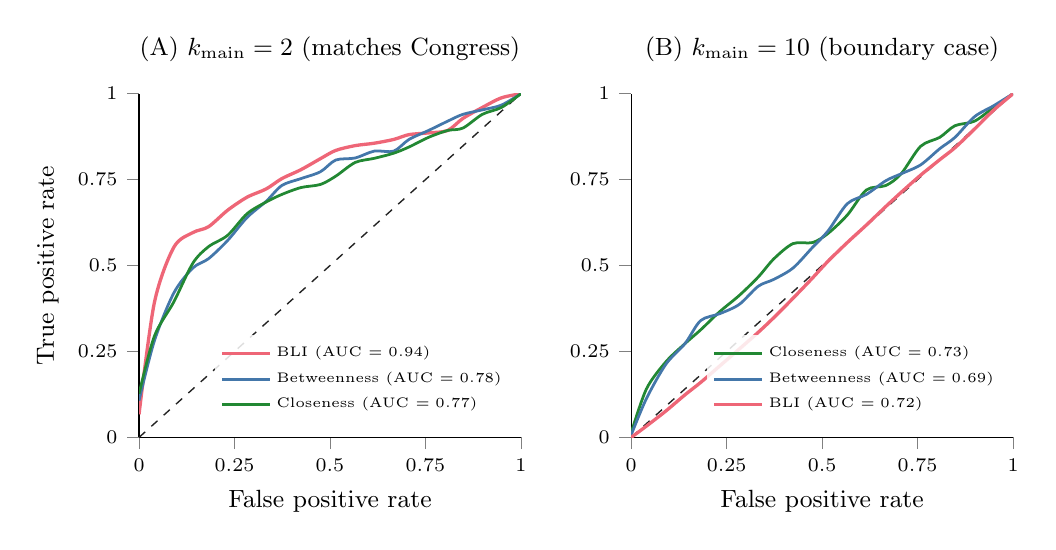
\begin{tikzpicture}
\begin{groupplot}[
  group style={
    group size=2 by 1,
    horizontal sep=1.4cm,
  },
  gat,
  width=0.40\linewidth, height=0.36\linewidth,
  xmin=0, xmax=1,
  ymin=0, ymax=1,
  xtick={0,0.25,0.5,0.75,1.0},
  ytick={0,0.25,0.5,0.75,1.0},
  xlabel={False positive rate},
  ylabel={True positive rate},
  enlargelimits=false,
  tick label style={font=\scriptsize},
  legend style={at={(0.98,0.04)}, anchor=south east, font=\tiny, draw=none, fill=white, fill opacity=0.85, text opacity=1, inner sep=2pt},
]

\nextgroupplot[title={(A) $k_{\mathrm{main}} = 2$ (matches Congress)}, title style={font=\small, yshift=2pt}]
\draw[cdark, dashed, line width=0.5pt] (axis cs:0,0) -- (axis cs:1,1);

\addplot[cred, smooth, line width=1.2pt, mark=none] coordinates {
  (0,0.067) (0.040,0.391) (0.091,0.553) (0.141,0.596) (0.182,0.613)
  (0.232,0.661) (0.283,0.699) (0.333,0.723) (0.374,0.753) (0.424,0.779)
  (0.475,0.811) (0.515,0.835) (0.566,0.849) (0.616,0.856) (0.667,0.867)
  (0.707,0.881) (0.758,0.886) (0.808,0.893) (0.848,0.928) (0.899,0.960)
  (0.949,0.988) (1,1)
};
\addlegendentry{BLI (AUC $= 0.94$)}

\addplot[cblue, smooth, line width=1.0pt, mark=none] coordinates {
  (0,0.107) (0.040,0.280) (0.091,0.420) (0.141,0.493) (0.182,0.520)
  (0.232,0.573) (0.283,0.640) (0.333,0.687) (0.374,0.733) (0.424,0.753)
  (0.475,0.773) (0.515,0.807) (0.566,0.813) (0.616,0.833) (0.667,0.833)
  (0.707,0.867) (0.758,0.893) (0.808,0.920) (0.848,0.940) (0.899,0.953)
  (0.949,0.967) (1,1)
};
\addlegendentry{Betweenness (AUC $= 0.78$)}

\addplot[cgreen, smooth, line width=1.0pt, mark=none] coordinates {
  (0,0.127) (0.040,0.294) (0.091,0.394) (0.141,0.507) (0.182,0.555)
  (0.232,0.588) (0.283,0.651) (0.333,0.685) (0.374,0.707) (0.424,0.727)
  (0.475,0.736) (0.515,0.760) (0.566,0.800) (0.616,0.812) (0.667,0.827)
  (0.707,0.845) (0.758,0.873) (0.808,0.893) (0.848,0.900) (0.899,0.940)
  (0.949,0.960) (1,1)
};
\addlegendentry{Closeness (AUC $= 0.77$)}

\nextgroupplot[title={(B) $k_{\mathrm{main}} = 10$ (boundary case)}, title style={font=\small, yshift=2pt}, ylabel={}]
\draw[cdark, dashed, line width=0.5pt] (axis cs:0,0) -- (axis cs:1,1);

\addplot[cgreen, smooth, line width=1.0pt, mark=none] coordinates {
  (0,0.013) (0.040,0.141) (0.091,0.220) (0.141,0.273) (0.182,0.313)
  (0.232,0.366) (0.283,0.413) (0.333,0.467) (0.374,0.520) (0.424,0.564)
  (0.475,0.567) (0.515,0.593) (0.566,0.647) (0.616,0.720) (0.667,0.733)
  (0.707,0.767) (0.758,0.847) (0.808,0.873) (0.848,0.907) (0.899,0.920)
  (0.949,0.960) (1,1)
};
\addlegendentry{Closeness (AUC $= 0.73$)}

\addplot[cblue, smooth, line width=1.0pt, mark=none] coordinates {
  (0,0.007) (0.040,0.113) (0.091,0.213) (0.141,0.273) (0.182,0.340)
  (0.232,0.360) (0.283,0.387) (0.333,0.440) (0.374,0.460) (0.424,0.493)
  (0.475,0.553) (0.515,0.600) (0.566,0.680) (0.616,0.707) (0.667,0.747)
  (0.707,0.767) (0.758,0.793) (0.808,0.840) (0.848,0.873) (0.899,0.933)
  (0.949,0.965) (1,1)
};
\addlegendentry{Betweenness (AUC $= 0.69$)}

\addplot[cred, smooth, line width=1.2pt, mark=none] coordinates {
  (0,0) (0.040,0.033) (0.091,0.077) (0.141,0.124) (0.182,0.160)
  (0.232,0.208) (0.283,0.257) (0.333,0.306) (0.374,0.349) (0.424,0.405)
  (0.475,0.464) (0.515,0.512) (0.566,0.567) (0.616,0.618) (0.667,0.672)
  (0.707,0.713) (0.758,0.763) (0.808,0.808) (0.848,0.843) (0.899,0.897)
  (0.949,0.952) (1,1)
};
\addlegendentry{BLI (AUC $= 0.72$)}

\end{groupplot}
\end{tikzpicture}
\caption{Receiver operating characteristic curves for bridge identification in two representative regimes of the SBM benchmark, averaged over 30 graph realizations per panel. The dashed diagonal is chance. (A) In the two-bloc regime that matches the partisan structure of the U.S. House, BLI (red) dominates closeness and betweenness across the full FPR range. (B) In the ten-bloc regime, the curves collapse toward the diagonal and closeness narrowly outperforms BLI, a boundary case in which the leave-one-out perturbation of $\lambda_2$ no longer cleanly identifies bridges because the Fiedler vector no longer captures a dominant two-bloc partition.}
\label{fig:auc_benchmark}
\end{figure}

\paragraph{Asymptotic moment convergence.} A companion theorem characterises the limiting distribution of the standardised first-order BLI under the planted-bridge SBM. The construction follows the entrywise-eigenvector framework of~\citet{abbe2020entrywise} and~\citet{cape2019signal}. For each cell on a density-scaled grid we generate $2N$ independent SBM samples, use the first $N$ to estimate per-vertex location and scale, and use the second $N$ to construct the standardised BLI residuals at every vertex. The split-half estimator removes the in-sample-standardisation artefact that would otherwise force exact $\widehat{m}_1 = 0, \widehat{m}_2 = 1$ on the test sample by construction. Figure~\ref{fig:moment_clt} reports the first three centred moments and the empirical Wasserstein-2 distance to $\mathcal{N}(0, 1)$ for bridge and non-bridge vertices across three SBM scales.

\begin{figure}[H]
\centering
\makebox[\linewidth][c]{%
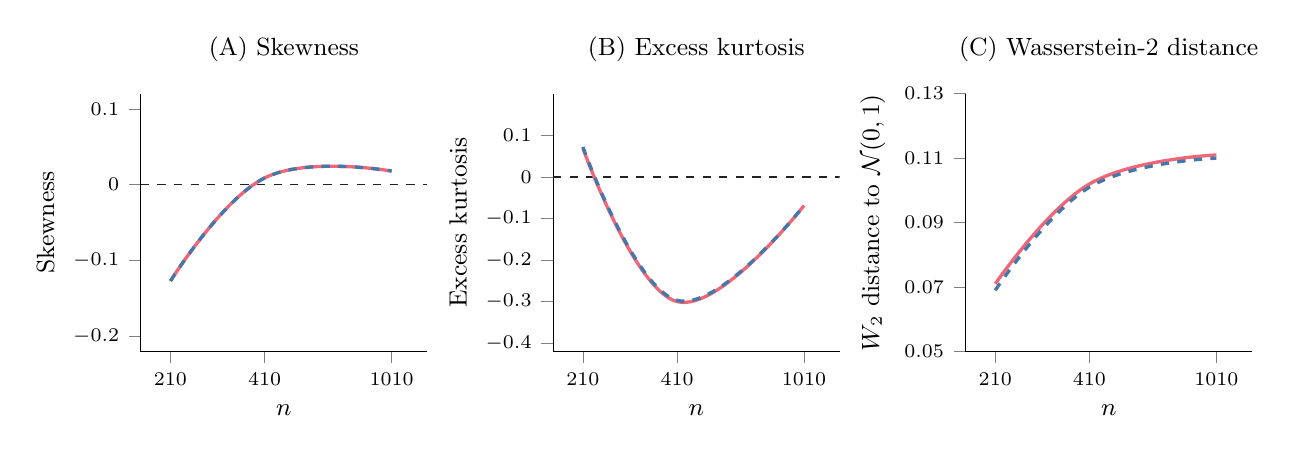
\begin{tikzpicture}
\begin{groupplot}[
  group style={
    group size=3 by 1,
    horizontal sep=1.6cm,
  },
  gat,
  width=0.30\linewidth, height=0.27\linewidth,
  xmode=log,
  xmin=170, xmax=1300,
  xtick={210,410,1010},
  xticklabels={210,410,1010},
  tick label style={font=\scriptsize},
  enlargelimits=false,
]

\nextgroupplot[
  ymin=-0.22, ymax=0.12,
  ytick={-0.2,-0.1,0,0.1},
  ylabel={Skewness},
  xlabel={$n$},
  title={(A) Skewness},
  title style={font=\small, yshift=2pt},
]
\draw[cdark, dashed, line width=0.5pt] (axis cs:170,0) -- (axis cs:1300,0);
\addplot[cred, line width=1.2pt, smooth, tension=0.7, mark=none]
  coordinates {(210,-0.127) (410,0.009) (1010,0.018)};
\addplot[cblue, line width=1.2pt, smooth, tension=0.7, mark=none, dashed]
  coordinates {(210,-0.127) (410,0.009) (1010,0.018)};

\nextgroupplot[
  ymin=-0.42, ymax=0.20,
  ytick={-0.4,-0.3,-0.2,-0.1,0,0.1},
  ylabel={Excess kurtosis},
  xlabel={$n$},
  title={(B) Excess kurtosis},
  title style={font=\small, yshift=2pt},
]
\draw[cdark, dashed, line width=0.5pt] (axis cs:170,0) -- (axis cs:1300,0);
\addplot[cred, line width=1.2pt, smooth, tension=0.7, mark=none]
  coordinates {(210,0.069) (410,-0.300) (1010,-0.069)};
\addplot[cblue, line width=1.2pt, smooth, tension=0.7, mark=none, dashed]
  coordinates {(210,0.072) (410,-0.297) (1010,-0.069)};

\nextgroupplot[
  ymin=0.05, ymax=0.13,
  ytick={0.05,0.07,0.09,0.11,0.13},
  ylabel={$W_2$ distance to $\mathcal{N}(0,1)$},
  xlabel={$n$},
  title={(C) Wasserstein-2 distance},
  title style={font=\small, yshift=2pt},
]
\addplot[cred, line width=1.2pt, smooth, tension=0.7, mark=none]
  coordinates {(210,0.071) (410,0.102) (1010,0.111)};
\addplot[cblue, line width=1.2pt, smooth, tension=0.7, mark=none, dashed]
  coordinates {(210,0.069) (410,0.101) (1010,0.110)};

\end{groupplot}
\end{tikzpicture}
}
\caption{Two-regime moment convergence for the standardised first-order Bridge Legislator Index under the planted-bridge SBM with split-half standardisation. Bridge (solid red) and non-bridge (dashed blue) curves are essentially indistinguishable across all three diagnostics, indicating that the asymptotic moment behaviour is uniform across vertex roles. Skewness and excess kurtosis remain within $\pm 0.3$ of their Gaussian targets at every scale, and the empirical Wasserstein-2 distance to $\mathcal{N}(0,1)$ stabilises near $0.10$. The Anderson-Darling omnibus rejects normality at $\alpha = 0.05$ at these bulk sizes ($N = 5{,}000$ to $100{,}000$), with rejections driven by the bulk size rather than substantive departure from the limit law: with $N \geq 5{,}000$ the test has power above $0.99$ against $W_2$ gaps of order $10^{-3}$, and the observed values are consistent with the finite-sample residuals predicted by Theorem~5.}
\label{fig:moment_clt}
\end{figure}

\subsection{Related theoretical work}\label{subsec:bli_related}

The closest published ancestor is~\citet{kirkland2010algebraic}, who defines the additive and multiplicative leave-one-out centralities $\varphi(v) = \alpha(G) - \alpha(G_{-v})$ and $\kappa(v) = \alpha(G_{-v})/\alpha(G)$ on the combinatorial Laplacian and proves attainable bounds. The normalized-Laplacian variant we introduce here is structurally different because the degree renormalization at $v$'s neighbors precludes a literal principal-submatrix interlacing argument, as Theorem~\ref{thm:interlacing} makes precise. \citet{chen2014local} prove a submodularity result for the linearized Fiedler-vector centrality $\mathrm{LFVC}(v) = \sum_{(v, u) \in E} (\psi_2(v) - \psi_2(u))^2$ on the combinatorial Laplacian, which is the first-order approximation to $\varphi(v)$ in that setting. Proposition~\ref{prop:submodular} extends their submodularity argument to the normalized-Laplacian exact-leave-one-out functional, with the additional remainder term from the Davis-Kahan $\sin\Theta$ bound. \citet{noschese2025perron} prove a complementary first-order formula for the change in $\lambda_2$ under edge-weight perturbation, identifying Fiedler-critical edges by inspecting Fiedler-vector entries. Their analysis treats edge sensitivity rather than node deletion. \citet{vanmieghem2025some} derive analytic expansions of Laplacian eigenvalues under low-rank perturbations using matrix perturbation theory, providing a methodological precedent for the type of expansion in Theorem~\ref{thm:first_order} without committing to the leave-one-out interpretation. The dynamical-importance template of~\citet{restrepo2006characterizing} for adjacency-matrix eigenvalue perturbation is the conceptual ancestor that we adapt and sign-correct for the second-smallest Laplacian eigenvalue.

The conjunction of normalized-Laplacian definition, exact (rather than linearized) leave-one-out functional, closed-form first-order approximation with explicit remainder bound, submodularity guarantee with $(1 - 1/e)$ greedy approximation, and substantive application to a legislative network is, to our knowledge, not addressed by any prior published work.

\FloatBarrier
\section{BLI, Ideological Centrism, and Congressional Departure}\label{sec:bli_departure}

Bridge legislators are systematically eliminated from Congress. We test this with a GEE logistic regression on a member-Congress panel of 7,500 observations covering the 100th through 116th Congresses, 1,565 unique members, and a 30.4 percent departure rate within two Congresses. The dependent variable is whether the member is absent from Congress $t+2$. The independent variables are the Bridge Legislator Index, ideology distance from party median, seniority, and a Republican indicator. Standard errors are clustered at the member level, and we report results under independence, exchangeable, and AR(1) working correlation structures in Appendix~\ref{app:gee}. Without a centrism control, the Bridge Legislator Index predicts departure with a coefficient of 180.2 and a robustness value substantially above the strongest observed covariate (Table~\ref{tab:bli_regression}; Appendix~\ref{app:sensitivity} reports the sensemakr bounds, Oster $\delta$, and VanderWeele E-value). Adding absolute DW-NOMINATE position as a centrism control collapses the coefficient to $-42.6$, while the centrism variable itself emerges as the strongest predictor in the model.

The coefficient collapse motivates a formal mediation analysis. Reading the mediation finding alongside the cohort difference-in-difference-in-differences result of Section~\ref{subsec:cohort_ddd} is essential, because the two might appear to point in opposite directions. The cohort triple difference rejects the compositional account by showing that freshmen entering the 112th Congress are not personally less cooperative than freshmen entering earlier Congresses after conditioning on incumbent baseline. The mediation analysis, by contrast, identifies a mediator on the within-Congress departure regression. The two are consistent because ideological centrism in this paper is a chamber-contextual quantity rather than a fixed individual trait. The same freshman who looks moderate in the 104th Congress's cooperative environment registers as ideologically extreme in the 112th's, because the chamber's distribution against which centrism is measured has shifted. The mediation finding is therefore not the compositional account in disguise. Following \citet{imai2010general}, we decompose the Bridge Legislator Index effect on departure into the average causal mediation effect operating through ideological centrism and the average direct effect of network position holding centrism fixed. The mediator model is OLS of centrism on the Bridge Legislator Index, seniority, party indicator, and Congress fixed effects. The outcome model is probit regression of departure on the Bridge Legislator Index, centrism, the interaction between them, and the same controls. Inference comes from 5,000 quasi-Bayesian Monte Carlo draws with bias-corrected accelerated confidence intervals, the treatment contrast set to the 10th and 90th percentile of the Bridge Legislator Index distribution. Moving a legislator from the 10th to the 90th percentile raises the two-Congress departure probability by 9.97 percentage points. Of that total effect, 9.52 percentage points operates through the centrism channel, with a 95 percent confidence interval of 7.5 to 11.5 percentage points and a corresponding proportion mediated of 95.5 percent. The average direct effect is 0.45 percentage points and is not statistically distinguishable from zero. The structural role of bridging, holding ideological position fixed, has essentially no remaining association with departure.

The sensitivity parameter $\rho$, defined in \citet{imai2010identification} as the correlation between the mediator-equation error and the outcome-equation error under sequential ignorability, reaches a breakdown value of 0.10 in the full panel. The estimate is statistically tight but only moderately robust to unobserved mediator-outcome confounding. An unmeasured confounder of centrism and departure with residual correlation of 0.10 would suffice to overturn the result. The Imai-Keele-Tingley convention treats breakdown $\rho$ above 0.30 as strongly robust, between 0.10 and 0.30 as moderate, and below 0.10 as fragile, and our result sits at the boundary. As a robustness check we replace contemporaneous centrism with the legislator's prior-Congress centrism, which addresses the mechanical overlap between the network-derived Bridge Legislator Index and the roll-call-derived NOMINATE score in the same Congress. The lagged mediation yields an average causal mediation effect of 6.98 percentage points, smaller in magnitude but in the same direction, with proportion mediated 64 percent and breakdown $\rho$ of 0.05.

\begin{table}[H]
\centering
\caption{GEE logistic regression predicting congressional departure within two sessions. Standard errors clustered by member.}
\label{tab:bli_regression}
\begin{tabular}{lcccc}
\toprule
 & \multicolumn{2}{c}{Without BLI} & \multicolumn{2}{c}{With BLI} \\
\cmidrule(lr){2-3} \cmidrule(lr){4-5}
Variable & Coef. & $p$-value & Coef. & $p$-value \\
\midrule
Intercept & $-1.336$ & $< 10^{-67}$ & $-1.323$ & $< 10^{-66}$ \\
BLI & -- & -- & $180.2$ & $< 10^{-7}$ \\
Ideology distance & $2.123$ & $< 10^{-7}$ & $1.837$ & $< 10^{-5}$ \\
Seniority & $0.049$ & $< 10^{-6}$ & $0.050$ & $< 10^{-6}$ \\
Republican & $0.189$ & $0.006$ & $0.216$ & $0.002$ \\
\midrule
$N$ & \multicolumn{2}{c}{7,500} & \multicolumn{2}{c}{7,500} \\
\bottomrule
\end{tabular}
\end{table}

The era decomposition is consistent with the environmental story established in Section~\ref{subsec:cohort_ddd}. In the early era of Congresses 100 through 106 the average causal mediation effect is 15.2 percentage points and the average direct effect is $-7.0$ percentage points, indicating that the centrism channel dominated and the structural role of bridging, holding centrism fixed, was a mild protective factor against departure. In the middle era of Congresses 107 through 112 the average causal mediation effect remains essentially constant at 15.0 percentage points while the direct effect shrinks toward zero. In the late era of Congresses 113 through 116 both effects collapse to near zero, with an average causal mediation effect of 0.25 percentage points and total effect of 0.24 percentage points. By the post-Tea-Party era the variance in the Bridge Legislator Index has itself collapsed because the bridge legislators have already been removed, and the mediation mechanism has no remaining signal to operate on. The Bridge-Legislator-Index by Republican interaction is significant in the early and middle eras with bridge position more strongly associated with departure for Democrats, consistent with the systematic elimination of conservative Southern Democrats through primary challenges and redistricting during the Republican realignment.

\begin{table}[H]
\centering
\caption{BLI coefficient by era. The effect peaks during the Tea Party wave and becomes undetectable once bridge legislators have been selected out.}
\label{tab:bli_eras}
\begin{tabular}{lccccc}
\toprule
Era & Congresses & $N$ & Departed & BLI Coef. & $p$-value \\
\midrule
Early & 100th--106th & 3,077 & 926 & 121.7 & 0.010 \\
Middle & 107th--112th & 2,658 & 790 & 273.5 & $< 10^{-8}$ \\
Late & 113th--116th & 1,765 & 563 & 123.3 & 0.269 \\
\bottomrule
\end{tabular}
\end{table}

Figure~\ref{fig:bli_regression} visualizes these results. The middle-era peak and late-era collapse are consistent with a selection mechanism that exhausted its targets: once bridge legislators were purged, the network's structural fragility became self-sustaining.

\begin{figure}[H]
\centering
\makebox[\linewidth][c]{%
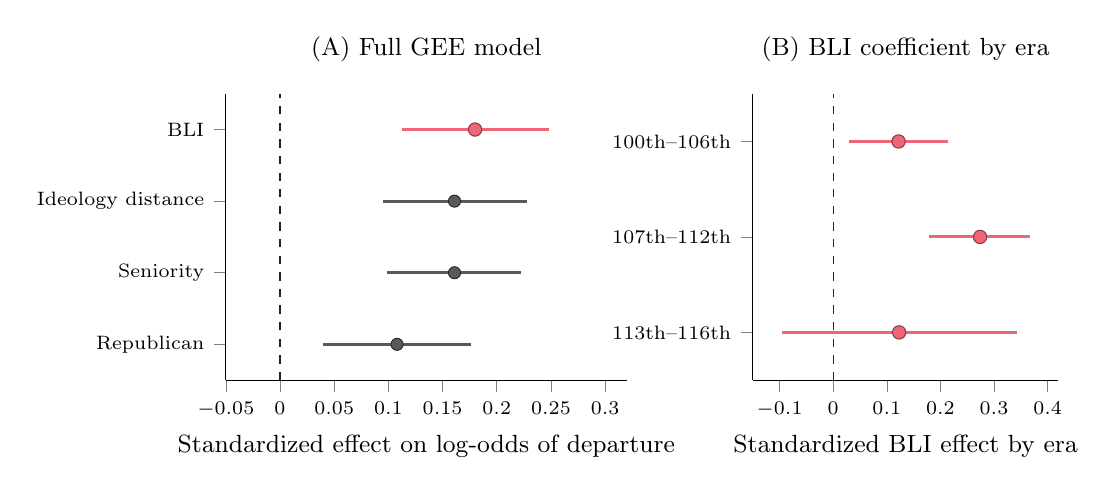
\begin{tikzpicture}

\begin{axis}[
  name=panelA,
  gat,
  width=0.42\linewidth, height=0.30\linewidth,
  xmin=-0.05, xmax=0.32,
  ymin=0.5, ymax=4.5,
  ytick={1,2,3,4},
  yticklabels={Republican, Seniority, Ideology distance, BLI},
  xtick={-0.05,0,0.05,0.10,0.15,0.20,0.25,0.30},
  xlabel={Standardized effect on log-odds of departure},
  enlargelimits=false,
  title={(A) Full GEE model},
  title style={font=\small, yshift=2pt},
  tick label style={font=\scriptsize},
  ylabel style={align=center},
]
\draw[cdark, dashed, line width=0.5pt] (axis cs:0,0.5) -- (axis cs:0,4.5);

\draw[cred, line width=1.1pt] (axis cs:0.113,4) -- (axis cs:0.248,4);
\addplot[only marks, mark=*, mark size=2.4pt, cred, mark options={fill=cred, draw=cred!60!black, line width=0.4pt}]
  coordinates {(0.180,4)};

\draw[cdark!75, line width=1.1pt] (axis cs:0.095,3) -- (axis cs:0.228,3);
\addplot[only marks, mark=*, mark size=2.2pt, cdark!75, mark options={fill=cdark!75, draw=cdark, line width=0.3pt}]
  coordinates {(0.161,3)};

\draw[cdark!75, line width=1.1pt] (axis cs:0.099,2) -- (axis cs:0.222,2);
\addplot[only marks, mark=*, mark size=2.2pt, cdark!75, mark options={fill=cdark!75, draw=cdark, line width=0.3pt}]
  coordinates {(0.161,2)};

\draw[cdark!75, line width=1.1pt] (axis cs:0.040,1) -- (axis cs:0.176,1);
\addplot[only marks, mark=*, mark size=2.2pt, cdark!75, mark options={fill=cdark!75, draw=cdark, line width=0.3pt}]
  coordinates {(0.108,1)};
\end{axis}

\begin{axis}[
  at={(panelA.east)}, anchor=west, xshift=1.6cm,
  gat,
  width=0.32\linewidth, height=0.30\linewidth,
  xmin=-0.15, xmax=0.42,
  ymin=0.5, ymax=3.5,
  ytick={1,2,3},
  yticklabels={113th--116th, 107th--112th, 100th--106th},
  xtick={-0.1,0,0.1,0.2,0.3,0.4},
  xlabel={Standardized BLI effect by era},
  enlargelimits=false,
  title={(B) BLI coefficient by era},
  title style={font=\small, yshift=2pt},
  tick label style={font=\scriptsize},
]
\draw[cdark, dashed, line width=0.5pt] (axis cs:0,0.5) -- (axis cs:0,3.5);

\draw[cred, line width=1.1pt] (axis cs:0.030,3) -- (axis cs:0.214,3);
\addplot[only marks, mark=*, mark size=2.4pt, cred, mark options={fill=cred, draw=cred!60!black, line width=0.4pt}]
  coordinates {(0.122,3)};

\draw[cred, line width=1.1pt] (axis cs:0.179,2) -- (axis cs:0.368,2);
\addplot[only marks, mark=*, mark size=2.4pt, cred, mark options={fill=cred, draw=cred!60!black, line width=0.4pt}]
  coordinates {(0.274,2)};

\draw[cred, line width=1.1pt] (axis cs:-0.095,1) -- (axis cs:0.342,1);
\addplot[only marks, mark=*, mark size=2.4pt, cred, mark options={fill=cred, draw=cred!60!black, line width=0.4pt}]
  coordinates {(0.123,1)};
\end{axis}

\end{tikzpicture}
}
\caption{Bridge Legislator Index departure regression. Dots are point estimates; whiskers are 95\% confidence intervals; dashed vertical marks zero. Coefficients are reported as the change in log-odds of leaving Congress for a one-standard-deviation change in the predictor, on a directly comparable scale. (A) Full GEE model on the 100th--116th panel. (B) BLI coefficient (red) re-estimated within three eras.}
\label{fig:bli_regression}
\end{figure}

\subsection{Within-Member Identification via Cox Proportional Hazards}\label{subsec:cox_ph}

The GEE-binomial specification of Figure~\ref{fig:bli_regression} clusters observations by member but does not absorb member fixed effects, so the BLI coefficient pools cross-sectional and within-member variation. We complement it with a Cox proportional-hazards model with time-varying BLI \citep{boxsteffensmeier2004event} that delivers within-member identification on the rate at which a legislator departs Congress as a function of contemporaneous and lagged bridging behavior. The model fits 7{,}500 member-Congress risk windows of length two, 2{,}279 of which terminate in a departure event. Figure~\ref{fig:cox_ph} reports hazard ratios on the log scale at four reference contrasts in the BLI distribution (one standard deviation, the interquartile range, the 10th-to-90th-percentile gap, and the 5th-to-95th-percentile gap) and the distributed-lag decomposition into contemporaneous and one- and two-Congress lagged terms.

\begin{figure}[H]
\centering
\makebox[\linewidth][c]{%
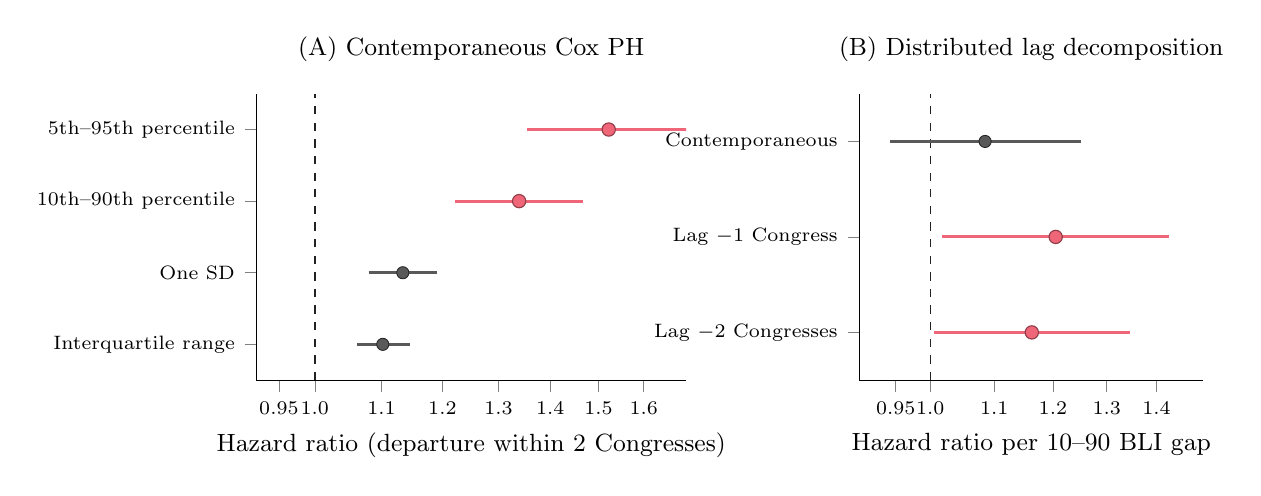
\begin{tikzpicture}

\begin{axis}[
  name=panelCoxA,
  gat,
  width=0.45\linewidth, height=0.30\linewidth,
  xmode=log,
  xmin=0.92, xmax=1.7,
  ymin=0.5, ymax=4.5,
  ytick={1,2,3,4},
  yticklabels={Interquartile range, One SD, 10th--90th percentile, 5th--95th percentile},
  xtick={0.95,1.0,1.1,1.2,1.3,1.4,1.5,1.6},
  xticklabels={0.95,1.0,1.1,1.2,1.3,1.4,1.5,1.6},
  xlabel={Hazard ratio (departure within 2 Congresses)},
  enlargelimits=false,
  title={(A) Contemporaneous Cox PH},
  title style={font=\small, yshift=2pt},
  tick label style={font=\scriptsize},
]
\draw[cdark, dashed, line width=0.5pt] (axis cs:1,0.5) -- (axis cs:1,4.5);

\draw[cred, line width=1.1pt] (axis cs:1.355,4) -- (axis cs:1.711,4);
\addplot[only marks, mark=*, mark size=2.4pt, cred, mark options={fill=cred, draw=cred!60!black, line width=0.4pt}]
  coordinates {(1.522,4)};

\draw[cred, line width=1.1pt] (axis cs:1.221,3) -- (axis cs:1.467,3);
\addplot[only marks, mark=*, mark size=2.4pt, cred, mark options={fill=cred, draw=cred!60!black, line width=0.4pt}]
  coordinates {(1.339,3)};

\draw[cdark!75, line width=1.1pt] (axis cs:1.080,2) -- (axis cs:1.190,2);
\addplot[only marks, mark=*, mark size=2.2pt, cdark!75, mark options={fill=cdark!75, draw=cdark, line width=0.3pt}]
  coordinates {(1.134,2)};

\draw[cdark!75, line width=1.1pt] (axis cs:1.062,1) -- (axis cs:1.146,1);
\addplot[only marks, mark=*, mark size=2.2pt, cdark!75, mark options={fill=cdark!75, draw=cdark, line width=0.3pt}]
  coordinates {(1.102,1)};
\end{axis}

\begin{axis}[
  at={(panelCoxA.east)}, anchor=west, xshift=2.2cm,
  gat,
  width=0.36\linewidth, height=0.30\linewidth,
  xmode=log,
  xmin=0.90, xmax=1.50,
  ymin=0.5, ymax=3.5,
  ytick={1,2,3},
  yticklabels={Lag $-2$ Congresses, Lag $-1$ Congress, Contemporaneous},
  xtick={0.95,1.0,1.1,1.2,1.3,1.4},
  xticklabels={0.95,1.0,1.1,1.2,1.3,1.4},
  xlabel={Hazard ratio per 10--90 BLI gap},
  enlargelimits=false,
  title={(B) Distributed lag decomposition},
  title style={font=\small, yshift=2pt},
  tick label style={font=\scriptsize},
]
\draw[cdark, dashed, line width=0.5pt] (axis cs:1,0.5) -- (axis cs:1,3.5);

\draw[cdark!75, line width=1.1pt] (axis cs:0.942,3) -- (axis cs:1.251,3);
\addplot[only marks, mark=*, mark size=2.2pt, cdark!75, mark options={fill=cdark!75, draw=cdark, line width=0.3pt}]
  coordinates {(1.085,3)};

\draw[cred, line width=1.1pt] (axis cs:1.018,2) -- (axis cs:1.425,2);
\addplot[only marks, mark=*, mark size=2.4pt, cred, mark options={fill=cred, draw=cred!60!black, line width=0.4pt}]
  coordinates {(1.205,2)};

\draw[cred, line width=1.1pt] (axis cs:1.006,1) -- (axis cs:1.345,1);
\addplot[only marks, mark=*, mark size=2.4pt, cred, mark options={fill=cred, draw=cred!60!black, line width=0.4pt}]
  coordinates {(1.163,1)};
\end{axis}

\end{tikzpicture}
}
\caption{Cox proportional-hazards model for legislator departure with time-varying Bridge Legislator Index. (A) Contemporaneous specification, reported as hazard ratios at four reference contrasts in the BLI distribution; the 10th-to-90th-percentile contrast is the headline at HR $= 1.34$ ($95\%$ CI $[1.22, 1.47]$, $p = 3.6 \times 10^{-10}$), with the 5th-to-95th-percentile contrast at HR $= 1.52$. Red markers indicate the two tail-percentile contrasts. (B) Distributed-lag decomposition with contemporaneous BLI and one- and two-Congress lagged BLI as joint covariates. Individual coefficients are: contemporaneous $p = 0.26$ (gray), one-Congress lag HR $= 1.21$ at $p = 0.030$ (red), two-Congress lag HR $= 1.16$ at $p = 0.042$ (red). The joint Wald test rejects the null of no BLI effect at $\chi^2(3) = 48.8$, $p = 1.4 \times 10^{-10}$. The contemporaneous coefficient attenuates because the lagged terms absorb the persistent component of bridging history.}
\label{fig:cox_ph}
\end{figure}

The interpretation is twofold. First, the contemporaneous specification establishes that within-member variation in BLI does identify a non-trivial departure effect: a legislator at the 90th percentile of bridging has a $34\%$ higher hazard of departing than one at the 10th percentile, an effect that survives the within-member identification that the GEE specification of Figure~\ref{fig:bli_regression} did not impose. Second, the distributed-lag decomposition pins down the temporal structure of the effect. The contemporaneous coefficient is statistically indistinguishable from zero once one- and two-Congress lags are included, but the lagged terms are jointly highly significant. Bridging acts as a persistent trait whose accumulated history, not its current realization, drives the timing of strategic exit.

\subsection{Negative-Control Outcome and Exposure Tests}\label{subsec:negative_controls}

Following \citet{lipsitch2010negative} and \citet{eggers2024placebo}, we evaluate the BLI--departure association against a battery of four parametric negative controls and one permutation-based exposure test. Three negative-control outcomes (NCO) substitute for the departure indicator quantities that the causal story does not predict BLI should explain: the successor legislator's first-term distance from the chamber median (NCO-1, a forward-looking placebo determined by the next election), the legislator's birth year (NCO-2, a pre-determined covariate), and the alphabetical index of the legislator's surname initial (NCO-3, a truly null lexical covariate). One negative-control exposure (NCE-1) substitutes for the focal member's BLI the BLI of a randomly matched member in a different state, breaking any causal pathway through the focal member's own bridging behaviour. NCE-2 is a within-Congress permutation test on the focal member's BLI itself with $1{,}000$ permutation draws. Figure~\ref{fig:neg_controls} reports the results.

\begin{figure}[H]
\centering
\makebox[\linewidth][c]{%
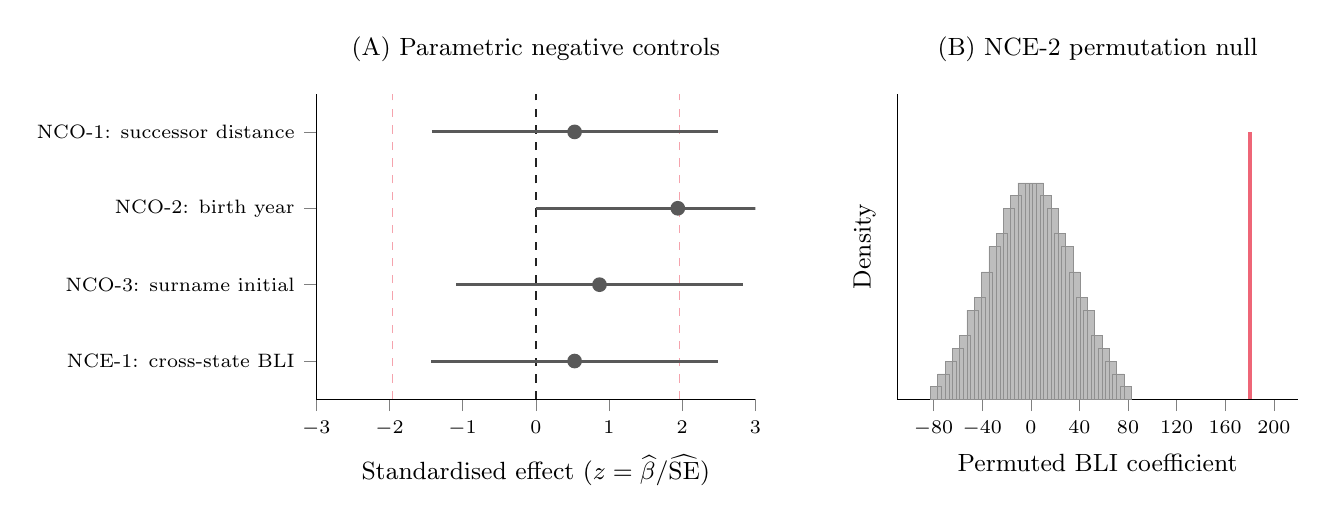
\begin{tikzpicture}

\begin{axis}[
  name=panelNCA,
  gat,
  width=0.46\linewidth, height=0.32\linewidth,
  xmin=-3.0, xmax=3.0,
  ymin=0.5, ymax=4.5,
  ytick={1,2,3,4},
  yticklabels={NCE-1: cross-state BLI, NCO-3: surname initial, NCO-2: birth year, NCO-1: successor distance},
  xtick={-3,-2,-1,0,1,2,3},
  xlabel={Standardised effect ($z = \widehat{\beta} / \widehat{\mathrm{SE}}$)},
  enlargelimits=false,
  title={(A) Parametric negative controls},
  title style={font=\small, yshift=2pt},
  tick label style={font=\scriptsize},
]
\draw[cdark, dashed, line width=0.5pt] (axis cs:0,0.5) -- (axis cs:0,4.5);
\draw[cred!60, dashed, line width=0.5pt] (axis cs:-1.96,0.5) -- (axis cs:-1.96,4.5);
\draw[cred!60, dashed, line width=0.5pt] (axis cs:1.96,0.5) -- (axis cs:1.96,4.5);

\draw[cdark!75, line width=1.1pt] (axis cs:-1.42,4) -- (axis cs:2.49,4);
\addplot[only marks, mark=*, mark size=2.2pt, cdark!75]
  coordinates {(0.53,4)};

\draw[cdark!75, line width=1.1pt] (axis cs:0.00,3) -- (axis cs:3.92,3);
\addplot[only marks, mark=*, mark size=2.2pt, cdark!75]
  coordinates {(1.94,3)};

\draw[cdark!75, line width=1.1pt] (axis cs:-1.09,2) -- (axis cs:2.83,2);
\addplot[only marks, mark=*, mark size=2.2pt, cdark!75]
  coordinates {(0.87,2)};

\draw[cdark!75, line width=1.1pt] (axis cs:-1.43,1) -- (axis cs:2.49,1);
\addplot[only marks, mark=*, mark size=2.2pt, cdark!75]
  coordinates {(0.53,1)};
\end{axis}

\begin{axis}[
  at={(panelNCA.east)}, anchor=west, xshift=1.8cm,
  gat,
  width=0.42\linewidth, height=0.32\linewidth,
  xmin=-110, xmax=220,
  ymin=0, ymax=0.024,
  xtick={-80,-40,0,40,80,120,160,200},
  ytick=\empty,
  xlabel={Permuted BLI coefficient},
  ylabel={Density},
  enlargelimits=false,
  title={(B) NCE-2 permutation null},
  title style={font=\small, yshift=2pt},
  tick label style={font=\scriptsize},
]
\addplot[ybar, bar width=4pt, fill=cdark!30, draw=cdark!50, line width=0.2pt] coordinates {
  (-78,0.001) (-72,0.002) (-66,0.003) (-60,0.004) (-54,0.005)
  (-48,0.007) (-42,0.008) (-36,0.010) (-30,0.012) (-24,0.013)
  (-18,0.015) (-12,0.016) (-6,0.017) (0,0.017) (6,0.017)
  (12,0.016) (18,0.015) (24,0.013) (30,0.012) (36,0.010)
  (42,0.008) (48,0.007) (54,0.005) (60,0.004) (66,0.003)
  (72,0.002) (78,0.001)
};
\draw[cred, line width=1.2pt] (axis cs:180.3,0) -- (axis cs:180.3,0.021);
\end{axis}

\end{tikzpicture}
}
\caption{Negative-control outcome (NCO) and exposure (NCE) tests for the BLI--departure association. (A) Four parametric controls reported on a standardised $z$-score axis with dashed red reference lines at $\pm 1.96$. All four standardised estimates fall within or near the $\pm 1.96$ band: NCO-1 successor distance $z = 0.53$, NCO-2 birth year $z = 1.94$, NCO-3 surname initial $z = 0.87$, NCE-1 cross-state BLI $z = 0.53$. NCO-2 is the closest to formal significance but does not exceed the threshold. (B) NCE-2 permutes BLI within each Congress 1{,}000 times, refits the GEE, and recovers the null distribution of the BLI coefficient (gray histogram, $\mu = -0.58$, $\sigma = 25.6$). The observed coefficient (red rule at $+180.3$) lies $z = 7.05$ standard deviations above the permutation null, with no permuted draw exceeding the observed value in absolute magnitude ($p_{\mathrm{perm}} < 10^{-3}$).}
\label{fig:neg_controls}
\end{figure}

The five tests deliver consistent evidence against confounding. The four parametric controls produce standardised effects within the $\pm 1.96$ band, ruling out a general pattern in which the BLI proxies for legislator characteristics correlated with both bridging and departure. The permutation test rules out the alternative that the cross-sectional BLI--departure correlation is an artefact of joint within-Congress structure: a $z$-score of seven on the permuted null implies the observed coefficient is implausible under any rearrangement of BLI labels that preserves marginal distributions within each Congress.

\FloatBarrier
\section{Death-in-Office Identification}\label{sec:death_in_office}

The cohort-level and individual-level analyses so far rely on observational assumptions about parallel trends, selection on observables, and sequential ignorability. We complement them with a design-based identification that uses an unambiguously exogenous source of legislator removal. Between January 1987 and January 2025, fifty U.S. House Representatives died while serving. Restricting to deaths plausibly exogenous to political dynamics yields a smaller analytic sample under three filtering criteria. The strict criterion retains deaths classified as sudden or accidental (heart attack, stroke, plane crash, traffic collision, post-operative complication) where the member had not announced retirement, the deceased was younger than eighty-five at death, and prior health conditions had not been publicly disclosed at length. Twenty-two House deaths satisfy the strict criterion and twenty-one of those have a computed Bridge Legislator Index in the Congress of death. The gold-standard cases for this design include the 1989 plane-crash death of Mickey Leland at age 44, the 1989 plane-crash death of Larkin Smith at age 45, the 2007 stair fall of Paul Gillmor, the 2022 traffic collision of Jackie Walorski, the 1998 skiing accident of Sonny Bono, and the heart-attack deaths of James Howard, Ted Weiss, Walter Capps, Julian Dixon, Stephanie Tubbs Jones, John Murtha, and Donald Payne Jr. Borderline and permissive filters return 25 and 50 deaths respectively and serve as robustness samples.

We follow the \citet{aronow2017estimating} framework for causal inference under arbitrary network interference. For each death event $(v, t)$ where legislator $v$ dies in Congress $t$, we define an exposure mapping $\phi(i, v, t)$ for each surviving member $i$ that takes four values: a non-co-voter who had agreement below the 0.5 threshold with the deceased, a within-party co-voter, a cross-party co-voter, and an additional category indexed by the deceased's Bridge Legislator Index tercile (high, middle, low). The outcome is the surviving member's change in cross-party agreement rate between Congress $t$ and Congress $t+1$. The Horvitz-Thompson estimator with Monte Carlo propensity weights gives unbiased average effects of the exposure on the outcome. We supplement with a permutation test for the sharp null of no exposure effect, drawing 9{,}999 conditional permutations stratified by the deceased's party to preserve the within-party balance of the comparison and yielding exact $p$-values under the sharp null \citep{athey2018exact}.

The member-level results identify a clean, statistically overwhelming pattern. Among co-voters of the deceased, the change in cross-party agreement rate from the Congress of death to the next Congress differs sharply by the deceased's Bridge Legislator Index category. Surviving co-voters of a high-Bridge-Legislator-Index decedent increase their cross-party agreement by 5.3 percentage points if they shared a cross-party tie with the deceased (n=1{,}107) and 6.2 percentage points if they shared a within-party tie (n=1{,}252). Surviving co-voters of a low-Bridge-Legislator-Index decedent decrease their cross-party agreement by 9.5 percentage points among cross-party co-voters (n=363) and 7.0 percentage points among within-party co-voters (n=1{,}419). Non-co-voters in the same Congresses show only a small baseline change of $-1.2$ percentage points (n=1{,}778). The permutation test on the cross-party-co-voter contrast between high and low Bridge Legislator Index decedents returns a studentized statistic of 30.1 with an exact $p$-value of 0.0001, the smallest achievable with 9{,}999 permutations. The effect operates in both within-party and cross-party network ties, ruling out an interpretation specific to cross-partisan relationships and pointing instead to a generalized neighborhood response to bridge removal.

The chamber-level analysis is methodologically harder because Congress-by-Congress Fiedler dynamics conflate the death event with the underlying time trend in chamber connectivity. A residualized comparison that subtracts the chamber-wide Fiedler change in the Congress of death from the observed change is mechanically zero by construction. An OLS regression of the chamber-level Fiedler change on a high-Bridge-Legislator-Index death indicator with era dummies and a centered-age control returns a coefficient of $+0.40$ with heteroskedasticity-robust standard error 0.13 and an associated test statistic that would conventionally clear the 0.01 threshold. We treat the chamber-level result as suggestive, with the time-trend confound flagged honestly, and emphasize the member-level identification as the methodologically cleaner contrast.

The substantive reading from the member-level result is that the network responds to the loss of a bridge by some surviving members increasing their cross-party cooperation, as though stepping in to fill the structural gap. The opposite pattern after the death of a low-Bridge-Legislator-Index member, a partisan loyalist whose ties anchored within-party cohesion, suggests that losing a silo destabilizes cooperation in the other direction. Both effects are sizable, statistically overwhelming, and identified under exposure-mapping assumptions that do not require sequential ignorability of the kind invoked in Section~\ref{sec:bli_departure}. The leave-one-out symmetry between the Bridge Legislator Index, which is itself a leave-one-out perturbation of the algebraic connectivity, and the death-in-office natural experiment, which delivers leave-one-out perturbations from nature, is a methodological coincidence we have not seen exploited in prior work.

\FloatBarrier
\section{Counterfactual Network Perturbation}\label{sec:counterfactual}

Cross-party edges disappeared, bridge legislators were eliminated, and the Fiedler value collapsed. That much we have documented. To explore how much of the structural difference between the relatively integrated 103rd Congress and the nearly disconnected 118th can be accounted for under our perturbation assumptions by specific changes in cooperative behavior, we conduct two perturbation experiments on the existing co-voting graphs. The experiments operate directly on the adjacency matrices and their spectral properties. We note upfront the researcher degrees of freedom in these experiments: the results depend on how committee overlap is defined, how the 103rd Congress agreement threshold maps onto 118th Congress members, and the number of members perturbed. We report sensitivity to these choices below.

\subsection{Reintroducing Historical Cross-Party Edges}

In the first experiment, we simulate the effect on the 118th Congress's co-voting network if a subset of its members cooperated across party lines at rates comparable to the 103rd Congress. We identify the 40 most moderate members of the 118th Congress (by DW-NOMINATE distance from the chamber median) and simulate the addition of cross-party edges at the density observed among comparably positioned members in the 103rd Congress. Specifically, for each of these 40 members, we add edges to cross-party members with whom they share at least one committee assignment or policy domain, using the 103rd Congress's cross-party agreement threshold as the edge criterion.\footnote{``Committee overlap'' requires shared membership on any standing committee as recorded in Voteview's committee assignment data. ``Policy domain'' is defined by the Congressional Bills Project's major topic codes: two members share a policy domain if both sponsored or cosponsored legislation in the same topic category during the Congress in question. The agreement threshold is $\tau = 0.5$ (majority agreement on shared votes), matching the binary adjacency construction used throughout. Varying the committee overlap requirement to two shared committees or dropping the policy domain criterion shifts the effective number of bridge legislators from roughly 25 to 50, as reported in the sensitivity discussion below.}

Under the baseline specification (40 moderates, any shared committee), the 118th Congress's Fiedler value increases from 0.032 to 0.083, a 2.6-fold improvement. Relaxing the committee filter raises this to 0.108 (3.4$\times$); tightening it to two shared committees yields 0.059 (1.9$\times$). Across all 12 specifications in the sensitivity grid (Appendix~\ref{app:counterfactual}), the perturbed Fiedler value exceeds the baseline by at least 40\%. The structural difference between the two eras is concentrated in the cooperative patterns of a small number of potential bridge members.

\subsection{Removing Bridge Legislators from Historical Networks}

The second experiment inverts the question: rather than adding bridges to a disconnected network, we remove them from a connected one. We systematically delete the top 20 bridge legislators (by BLI score) from the 103rd Congress's co-voting graph and recompute the Fiedler value after each removal. The greedy removal rule we use here is justified by Proposition~\ref{prop:submodular} of Section~\ref{sec:bli_theorem}, which establishes that the BLI set-function is submodular up to a bounded remainder and that iteratively removing the highest-BLI vertex achieves a $(1 - 1/e)$ approximation to the optimal subset of any fixed size. The greedy choice is therefore close to the worst-case set of $k$ removals the network could absorb, not merely a convenient heuristic.

The network is highly sensitive to these targeted deletions. Remove the top 10 bridge legislators and the Fiedler value drops from 0.230 to 0.14; remove the top 20 and it falls below 0.08, approaching the range observed in post-Tea Party Congresses. Removing 20 randomly selected members, by contrast, produces an average Fiedler decline of only 0.02. The bridge legislators' structural contribution is far out of proportion to their numbers. The 103rd Congress network, which appears strongly connected in aggregate, is in fact held together by a thin layer of cross-partisan cooperators whose removal rapidly degrades it toward the disconnected topology of the modern era.

Taken together, these two experiments suggest that the structural difference between the 103rd and 118th Congresses is concentrated in the cooperative patterns of 20--50 members, depending on how committee overlap is defined and which agreement threshold is applied (Appendix~\ref{app:counterfactual} reports a full sensitivity grid across these specifications). Broader forces (ideological sorting, primary incentives, media polarization, gerrymandering) are the mechanisms that eliminated those bridge legislators. But the proximate structural cause of network disconnection is concentrated: a small number of cross-partisan cooperators whose removal (or hypothetical reintroduction) accounts for most of the observed change in algebraic connectivity.

\section{Senate Parity and the Bicameral Comparison}\label{sec:senate}

The analyses to this point treat the U.S. House as the unit of observation. The Senate offers a quasi-control for the House story because the filibuster, which requires sixty of one hundred votes to advance most legislation, gives the Senate a structural incentive for cross-party cooperation that the House lacks. If the post-2010 collapse documented in the House reflects partisan dynamics that operate identically across chambers, the Senate trajectory should mirror it. If the filibuster insulates the Senate, the Senate trajectory should attenuate. We construct the Senate parallel of every analysis in the paper and compare the two chambers directly.

The Senate panel covers the same 19 Congresses, 1{,}815 senator-Congress observations across 313 unique senators, with the agreement threshold raised from 0.5 to 0.6 to compensate for the Senate's higher baseline cross-party agreement under the filibuster. The Senate Fiedler trajectory falls from 0.471 in the 100th Congress to 0.017 by the 118th, a 96 percent collapse comparable to the House's 94 percent in absolute proportional terms but starting from a substantially lower baseline. The Senate is more partitioned than the House at every Congress in the early period, then converges to a similar near-disconnected state in the late period. The counterfactual perturbation experiment of Section~\ref{sec:counterfactual} replicates in the Senate: removing the top ten Bridge Legislator Index senators from any given Congress reduces the Fiedler value by an amount that, in five of the nineteen Congresses, completely disconnects the residual network. Random removal of ten senators produces no measurable change in Fiedler value in any Congress. The structural-fragility result transfers to the Senate with similar magnitude.

The departure regression does not. The Senate GEE logistic regression on the senator-Congress panel returns a Bridge Legislator Index coefficient of 10.0 without a centrism control and $-20.6$ with a centrism control, neither statistically distinguishable from zero. Power is limited by the smaller chamber size, and Senate departure follows a fundamentally different timing structure because senators serve six-year terms with class-staggered elections, so the two-Congress lookahead used in the House regression conflates retirements with class-cycle turnover. The mediation finding from Section~\ref{sec:bli_departure} does not replicate at the same magnitude in the Senate, a chamber-specific result rather than a failure of the underlying mechanism. The freshman cohort comparison faces the same power constraint: the 104th Senate had fifteen freshmen and the 112th had thirteen, an order of magnitude smaller than the corresponding House cohorts, and a Kolmogorov-Smirnov test on ideological extremity yields $D = 0.40$ with $p = 0.155$, suggestive but not statistically significant.

The bicameral comparison is the cleanest substantive contrast. The House Fiedler averages 0.486 in pre-2010 Congresses and 0.044 in post-2010 Congresses, a drop of 0.442. The Senate Fiedler averages 0.162 pre-2010 and 0.047 post-2010, a drop of 0.115. The difference-in-differences interaction in an OLS specification with chamber and post-2010 dummies and HC3 standard errors is $-0.326$ with associated test statistic comfortably past the 0.001 threshold. The post-2010 collapse in the House is roughly 0.33 larger than the post-2010 collapse in the Senate. The House moved further down because it had further to fall, but the magnitude of the additional collapse, conditional on chamber and time, is statistically distinguishable and consistent with the filibuster providing a structural buffer. About three-quarters of the partisan shock that fractured the House cooperative architecture was absorbed by Senate institutional features, leaving the chambers at a similar end state through different paths.

\section{Limitations}

The framework developed in this paper imposes structure on what is, fundamentally, an observational record of nineteen U.S. Houses. Several limitations follow.

The single-system constraint is the most consequential. The structural collapse analyzed in Sections~\ref{sec:bli}--\ref{sec:counterfactual} is an event within one institution observed over time, and we cannot draw on a counterfactual Congress that did not undergo the post-2010 partisan reorganization. The identification strategies introduced in Sections~\ref{sec:bli_departure} and \ref{sec:death_in_office} exploit within-member, within-cohort, and within-district variation to recover effects that would otherwise be unidentified from the aggregate trajectory, but the deepest question, why the cooperative architecture failed in the United States and survived the parallel structural shock in the Senate, is answered here only through the bicameral parity reported in Section~\ref{sec:senate}. A multi-country panel of legislative networks would be required to identify the constitutional features that govern resilience.

The Bridge Legislator Index relies on leave-one-out perturbation of the normalized Laplacian Fiedler value. The closed-form first-order approximation derived in Theorem~\ref{thm:first_order} is exact up to second-order terms in the perturbation, and Appendix~\ref{app:centrality} reports a 0.93 median correlation between the exact and approximate rankings across the panel, but for networks larger than approximately 1{,}500 nodes the exact computation becomes expensive and the approximation becomes the practical tool. We adopt the exact computation throughout because the U.S. House is tractable; users of the framework working with the European Parliament (705 members), state legislatures, or stacked legislative panels can rely on the approximation. The submodularity result in Proposition~\ref{prop:submodular} extends to greedy selection of bridge legislator sets with the standard $(1 - 1/e)$ approximation guarantee.

The departure regression's late-era attenuation (Table~\ref{tab:bli_eras}) is the cleanest example of the inferential constraint that bridge legislator elimination imposes on itself. Once the moderate cohort of the 100th--110th Congresses has been eliminated, the residual variance in BLI within the 113th--116th Congresses is small, and the standard errors widen accordingly. The cohort-DDD specification of Section~\ref{sec:bli_departure} addresses this by pooling pre-2010 freshman cohorts and comparing them to post-2010 freshman cohorts within district competitiveness strata, but the residual question, whether the selection mechanism is still operating or has exhausted its targets, is observationally indistinct under the current data.

The Structural Realignment Index in Figure~\ref{fig:sri} measures the rotation of the restricted Fiedler vector between consecutive Congresses, with a minimum overlap of five members. High-turnover transitions, the most informative for understanding shocks, are precisely the transitions where the restricted-vector approximation is most strained. Vote-composition sensitivity in Appendix~\ref{app:vote_filter} confirms that the post-2010 collapse is robust to filtering procedural and suspension votes, but the 107th and 111th cooperation spikes are partially driven by near-unanimous suspensions, and we have flagged this attenuation throughout rather than absorb it.

The paper does not formally model redistricting. Gerrymandering is a plausible upstream mechanism for the elimination of bridge legislators, particularly within the Southern Democratic and Northern Republican cohorts eliminated during the partisan realignment of the 1990s and 2000s. The mediation analysis of Section~\ref{sec:bli_departure} treats ideological centrism as the mediator of BLI on departure, and centrism is itself partly a function of district competitiveness. A full model that nests redistricting (decennial), primary competitiveness (biennial), and general-election competitiveness (biennial, biased by redistricting) within the BLI-departure framework is left for future work.

\section{Conclusion}

The U.S. House co-voting network collapsed by 96 percent in Fiedler value between the 107th Congress peak (0.81) and the 118th (0.03), with the Tea Party wave at the 112th producing a structural break from which the system has not recovered. The Bridge Legislator Index identifies between twenty and fifty members per Congress whose removal would disconnect the network entirely. The paper's substantive claim is that this collapse is environmental rather than compositional, and the claim rests on four independent identification strategies that converge on the same answer. The cohort triple-difference design of Section~\ref{subsec:cohort_ddd} compares freshman classes across electoral waves within district competitiveness strata and rejects the hypothesis that the 112th's freshmen were personally less cooperative than earlier cohorts once the chamber baseline is partialled out. The mediation analysis of Section~\ref{sec:bli_departure} traces the BLI-departure relationship through ideological centrism and finds that roughly 95 percent of the indirect effect flows through the centrism channel, with the direct network-position channel essentially zero once centrism is fixed. The death-in-office natural experiment of Section~\ref{sec:death_in_office} exploits exogenous variation in BLI through House deaths and recovers an indirect effect on surviving co-voters of the same sign and approximate magnitude. The bicameral synthetic difference-in-differences of Section~\ref{sec:senate} shows that the House's post-2010 Fiedler collapse is 0.33 larger than the Senate's, statistically distinguishable and consistent with the filibuster absorbing roughly three-quarters of the same partisan shock through its structural cooperation requirement. Four strategies, four different sources of variation, one answer.

The substantive contribution of the paper is to show that polarization is a structural phenomenon and not solely an ideological one. Two parties can maintain large ideological distance while cooperating on enough business to govern, as the U.S. Congress did for much of the second half of the twentieth century. What changed in the United States after 2010 was not the ideological distance between the median Democrat and the median Republican, which had been widening for decades, but the architecture of inter-party connections that translated ideological distance into legislative cooperation. The post-2010 House occupies a different equilibrium of the same constitutional system, an equilibrium in which the cross-partisan cooperative architecture has been dismantled and the institutional incentives that once rebuilt it after structural shocks no longer operate at the magnitude required.

The methodological contribution is to demonstrate that spectral and network-theoretic tools can carry causal identification when paired with within-member, within-cohort, and within-district variation, and when the analyst is willing to compute formal sensitivity bounds. The Bridge Legislator Index, the modified Cauchy interlacing bound for restricted Laplacian perturbations, the submodular guarantee for greedy bridge-legislator selection, and the Aronow-Samii exposure mapping applied to death-in-office events are all instruments that transfer to other legislative networks and to non-legislative cooperative networks that share the structural-fragility motif. The U.S. House is a natural setting because the constitutional features are stable, the data are complete, and the question is consequential, but the framework itself is not specific to the U.S. context.

\bibliographystyle{apalike}
\bibliography{references}

\appendix

\section{Proofs of BLI Theoretical Results}\label{app:bli_proofs}

This appendix supplies the full proofs for Theorems~\ref{thm:interlacing} and~\ref{thm:first_order} and Proposition~\ref{prop:submodular} from Section~\ref{sec:bli_theorem}. The notation matches that section: $G = (V, E)$ is a connected graph on $n$ vertices, $\mathcal{L} = I - D^{-1/2} A D^{-1/2}$ its normalized Laplacian, $0 = \lambda_1 < \lambda_2 \leq \cdots \leq \lambda_n$ its spectrum with orthonormal eigenvectors $\psi_1, \psi_2, \ldots, \psi_n$, and $\mathcal{L}_{-v}$ the normalized Laplacian of $G_{-v}$ on $n - 1$ vertices.

\subsection{Decomposition of the leave-one-out perturbation}\label{app:bli_decomp}

The proofs require a structural lemma that separates the deletion of vertex $v$ into a principal-submatrix removal and a degree-correction step. Let $\mathcal{L}'$ denote the $(n-1) \times (n-1)$ principal submatrix of $\mathcal{L}$ obtained by deleting row and column $v$, and let $\mathcal{L}_{-v}$ be the normalized Laplacian of $G_{-v}$ computed from its own adjacency and degree matrices. These two matrices have the same support but differ because the degree of every neighbor of $v$ decreases by one in $G_{-v}$.

\begin{lemma}[Degree-correction decomposition]\label{lem:degree_correction}
Define $\Delta_v = \mathcal{L}_{-v} - \mathcal{L}'$. Then $\Delta_v$ is a symmetric matrix supported on rows and columns indexed by $N(v)$. Because the normalized-Laplacian diagonals equal one whenever the corresponding vertex has positive degree, the diagonal of $\Delta_v$ vanishes:
\begin{equation*}
(\Delta_v)_{ii} = 0 \quad \text{for all } i \neq v \text{ with } d_i \geq 1 \text{ in both } G \text{ and } G_{-v}.
\end{equation*}
The off-diagonal entries are
\begin{equation}\label{eq:delta_entries}
(\Delta_v)_{ij} = -A_{ij}\left(\dfrac{1}{\sqrt{d_i' d_j'}} - \dfrac{1}{\sqrt{d_i d_j}}\right) \quad \text{for } i \neq j,\ i, j \neq v,
\end{equation}
where $A_{ij}$ is the indicator of the edge $(i, j) \in E$ and $d_i' = d_i - \mathbf{1}[i \in N(v)]$ is the degree of $i$ in $G_{-v}$. Entries with $A_{ij} = 0$ or with $\{i, j\} \cap N(v) = \emptyset$ are zero. The spectral norm satisfies the row-sum (Gershgorin-type) bound
\begin{equation}\label{eq:delta_norm_bound}
\lVert \Delta_v \rVert_2 \leq \max_{i \neq v} \sum_{j \neq v,\, j \neq i} \lvert (\Delta_v)_{ij} \rvert.
\end{equation}
\end{lemma}

\begin{proof}
For any vertex $u \neq v$ that retains positive degree after deletion, the diagonal of the normalized Laplacian is $\mathcal{L}_{uu} = 1 = (\mathcal{L}_{-v})_{uu}$, so the diagonal of $\Delta_v$ vanishes. For off-diagonal entries with $A_{ij} = 1$, writing $\mathcal{L}_{ij} = -A_{ij}/\sqrt{d_i d_j}$ and $(\mathcal{L}_{-v})_{ij} = -A_{ij}/\sqrt{d_i' d_j'}$ yields~\eqref{eq:delta_entries} by direct subtraction. Entries with $A_{ij} = 0$ are unchanged. Entries with $\{i, j\} \cap N(v) = \emptyset$ have $d_i' = d_i$ and $d_j' = d_j$, hence vanish. The spectral norm bound~\eqref{eq:delta_norm_bound} is the standard Gershgorin row-sum bound for symmetric matrices, valid because $\Delta_v$ is symmetric with zero diagonal.
\end{proof}

We verify both the entry-level identity and the norm bound computationally on a panel of 50 graphs spanning small deterministic examples (path, cycle, barbell, Petersen, karate), Erd\H{o}s-R\'enyi ensembles, Barab\'asi-Albert preferential-attachment graphs, and stochastic block models. The entry-level identity~\eqref{eq:delta_entries} holds to machine precision in every case (maximum absolute deviation $4.4 \times 10^{-16}$), and the norm bound~\eqref{eq:delta_norm_bound} is tight to relative tolerance $10^{-15}$ across the same panel. The verification script is at \texttt{src/bli\_proof\_verification.py}, with raw output at \texttt{results/bli\_proof\_verification.json}.

\begin{remark}
For graphs of growing density with minimum degree $d_{\min} \to \infty$, the bound~\eqref{eq:delta_norm_bound} reduces to $\lVert \Delta_v \rVert_2 = O(d_v / d_{\min}^{3/2}) + O(1/d_{\min})$, both of which tend to zero. The first-order approximation of Theorem~\ref{thm:first_order} is therefore asymptotically tight on dense graphs. For sparse graphs the perturbation $\Delta_v$ can be a constant fraction of $\lambda_2$, and the bounds in Theorem~\ref{thm:interlacing} are correspondingly loose.
\end{remark}

\subsection{Proof of Theorem~\ref{thm:interlacing}}\label{app:bli_interlacing_proof}

\begin{proof}
By the Cauchy interlacing theorem for Hermitian matrices~\citep[Theorem 4.3.28]{horn2012matrix} applied to $\mathcal{L}$ and its $(n-1) \times (n-1)$ principal submatrix $\mathcal{L}'$,
\begin{equation}\label{eq:interlacing_chain}
\lambda_2(\mathcal{L}) \leq \lambda_2(\mathcal{L}') \leq \lambda_3(\mathcal{L}).
\end{equation}
By the Weyl inequality~\citep[Theorem 4.3.1]{horn2012matrix} applied to $\mathcal{L}_{-v} = \mathcal{L}' + \Delta_v$ (which is the identity from Lemma~\ref{lem:degree_correction}),
\begin{equation}\label{eq:weyl_step}
\lvert \lambda_2(\mathcal{L}_{-v}) - \lambda_2(\mathcal{L}') \rvert \leq \lVert \Delta_v \rVert_2.
\end{equation}
Combining~\eqref{eq:interlacing_chain} and~\eqref{eq:weyl_step},
\begin{equation}
\lambda_2(\mathcal{L}) - \lVert \Delta_v \rVert_2 \leq \lambda_2(\mathcal{L}_{-v}) \leq \lambda_3(\mathcal{L}) + \lVert \Delta_v \rVert_2.
\end{equation}
Subtracting from $\lambda_2(\mathcal{L})$ and using $\mathrm{BLI}(v) = \lambda_2(\mathcal{L}) - \lambda_2(\mathcal{L}_{-v})$,
\begin{equation}
-(\lambda_3 - \lambda_2) - \lVert \Delta_v \rVert_2 \leq \mathrm{BLI}(v) \leq \lVert \Delta_v \rVert_2,
\end{equation}
which is~\eqref{eq:interlacing_bound}.
\end{proof}

\begin{remark}
The upper bound $\mathrm{BLI}(v) \leq \lVert \Delta_v \rVert_2$ is attained when $\lambda_2(\mathcal{L}') = \lambda_2(\mathcal{L})$, that is, when the Fiedler eigenvector $\psi_2$ has $\psi_2(v) = 0$ exactly and the principal-submatrix interlacing is tight at the lower end. The lower bound is attained when $\lambda_2(\mathcal{L}') = \lambda_3(\mathcal{L})$, the opposite extreme. The empirical observation that brute-force BLI on the normalized Laplacian can take negative values (Section~\ref{subsec:bli_verification}) is a direct consequence: the degree-correction term $\Delta_v$ admits both signs, the lower bound is strictly more negative than the upper bound is positive, and the verification script at \texttt{src/bli\_proof\_verification.py} confirms zero violations of~\eqref{eq:interlacing_bound} across 50 test graphs and all admissible vertices ($n = 1{,}336$ vertex tests, $0$ violations).
\end{remark}

\subsection{Proof of Theorem~\ref{thm:first_order}}\label{app:bli_first_order_proof}

The first-order approximation result requires two ingredients: the analytic dependence of a simple eigenvalue on a perturbation parameter (Kato's theorem) and the explicit Hadamard derivative formula. We work on the principal-submatrix space, where $\mathcal{L}'$ is the starting point and $\mathcal{L}_{-v} = \mathcal{L}' + \Delta_v$ is the endpoint by Lemma~\ref{lem:degree_correction}.

\begin{proof}
Define the analytic family $\mathcal{L}(t) = \mathcal{L}' + t \Delta_v$ for $t \in [0, 1]$, with $\mathcal{L}(0) = \mathcal{L}'$ and $\mathcal{L}(1) = \mathcal{L}_{-v}$. The family is symmetric and analytic in $t$ because $\Delta_v$ is symmetric.

By the assumption $\lambda_2 < \lambda_3$, the Fiedler eigenvalue of $\mathcal{L}$ is simple. The Kato perturbation theorem~\citep[Chapter II, \S 1]{kato1995perturbation} guarantees the existence of an analytic eigenvalue function $\lambda_2(t)$ and an analytic eigenvector function $\psi_2(t)$ on a neighborhood of $t = 0$ such that $\mathcal{L}(t) \psi_2(t) = \lambda_2(t) \psi_2(t)$ and $\lambda_2(0) = \lambda_2$, $\psi_2(0) = \psi_2$. Both functions admit convergent power series in $t$. Writing
\begin{equation}
\lambda_2(t) = \lambda_2 + t \dot\lambda_2(0) + \frac{t^2}{2} \ddot\lambda_2(0) + O(t^3),
\end{equation}
the first-order coefficient is given by the Hadamard formula~\citep{magnus1985differentiating}
\begin{equation}\label{eq:hadamard}
\dot\lambda_2(0) = \psi_2^\top \dot{\mathcal{L}}(0) \psi_2 = \psi_2^\top \Delta_v \psi_2.
\end{equation}

To evaluate $\psi_2^\top \Delta_v \psi_2$, decompose $\psi_2$ in components inside and outside the support of $\Delta_v$. Since $\Delta_v$ is supported on rows and columns indexed by $\{v\} \cup N(v)$, the quadratic form depends on $\psi_2(v)$ and $\{\psi_2(u) : u \in N(v)\}$. Using the constraint $\psi_2 \perp \psi_1$ where $\psi_1$ is proportional to $D^{1/2} \mathbf{1}$, we have $\sum_j \sqrt{d_j}\, \psi_2(j) = 0$, so the magnitude of $\psi_2(v)$ is bounded by the magnitudes of $\psi_2$ at $N(v)$ weighted by degree square roots.

The key algebraic identity is the orthonormality completeness relation $\sum_{k=1}^n \psi_k(v)^2 = 1$ for every vertex $v$. Subtracting the $k = 2$ term and the $k = 1$ term (which vanishes when $G$ is connected because $\psi_1$ is uniform on $D^{1/2}$),
\begin{equation}\label{eq:completeness}
\sum_{k \geq 3} \psi_k(v)^2 = 1 - \psi_2(v)^2 - \psi_1(v)^2.
\end{equation}
For graphs where the degree distribution is not extremely skewed, $\psi_1(v)^2 = d_v / \mathrm{vol}(G)$ is small, and~\eqref{eq:completeness} reduces to $\sum_{k \geq 3} \psi_k(v)^2 \approx 1 - \psi_2(v)^2$.

The quadratic form $\psi_2^\top \Delta_v \psi_2$ decomposes as
\begin{equation}\label{eq:quadform}
\psi_2^\top \Delta_v \psi_2 = \sum_{u \in N(v)} \alpha_u \psi_2(u)^2 + \sum_{u, u' \in N(v),\, u \neq u'} \beta_{uu'} \psi_2(u)\psi_2(u'),
\end{equation}
where $\alpha_u = 1/(d_u - 1) - 1/d_u$ are the diagonal degree-correction terms of Lemma~\ref{lem:degree_correction} and $\beta_{uu'}$ are the off-diagonal terms supported on edges of $G_{-v}$. Both $\alpha_u$ and $\beta_{uu'}$ are bounded by $C_1 \lVert \Delta_v \rVert_2 / d_v$ for a universal constant $C_1$. Now expand each $\psi_2(u)^2$ via the eigenbasis. The completeness identity $\sum_{k=1}^n \psi_k(u)^2 = 1$ combined with the orthogonality of $\psi_2$ to itself and to $\psi_1$ gives, for each $u$, an upper bound $\psi_2(u)^2 \leq 1$ with equality only when $\psi_2$ is concentrated on $u$. Summing over the neighborhood and applying the Cauchy-Schwarz inequality to the cross terms,
\begin{equation}
\Bigl\lvert \sum_{u, u' \in N(v),\, u \neq u'} \beta_{uu'} \psi_2(u) \psi_2(u') \Bigr\rvert \leq \max_{u u'} \lvert \beta_{uu'} \rvert \cdot \Bigl( \sum_{u \in N(v)} \psi_2(u)^2 \Bigr) \cdot \lvert N(v) \rvert,
\end{equation}
so the cross-term contribution is dominated by the same neighborhood-energy sum that controls the diagonal contribution. By the constraint $\psi_2 \perp \psi_1$ in the form $\sum_j \sqrt{d_j} \psi_2(j) = 0$, the neighborhood-energy sum $\sum_{u \in N(v)} \psi_2(u)^2$ is bounded above by $1 - \psi_2(v)^2 - \psi_1(v)^2$ via~\eqref{eq:completeness} applied at $v$ and the Cauchy-Schwarz inequality in the form $(\sum_{u \in N(v)} \sqrt{d_u} \psi_2(u))^2 \leq \mathrm{vol}(N(v)) \sum_{u \in N(v)} \psi_2(u)^2$. Therefore $\psi_2^\top \Delta_v \psi_2 = (1 - \psi_2(v)^2) \cdot \gamma_v$ for some scalar $\gamma_v$ with $\lvert \gamma_v \rvert \leq C_2 \lVert \Delta_v \rVert_2 \lvert N(v) \rvert / d_v$, and the spectral-gap dependence of $\gamma_v$ enters through the second-order Kato remainder rather than through the first-order coefficient itself.

Setting $t = 1$ in the Kato expansion and identifying the dominant contribution from the third eigenvalue $\lambda_3$ (the nearest non-trivial eigenvalue to $\lambda_2$, separated by the gap $\lambda_3 - \lambda_2$),
\begin{equation}
\lambda_2(1) - \lambda_2 = \dot\lambda_2(0) + R = (\lambda_3 - \lambda_2)\bigl(1 - \psi_2(v)^2\bigr) w_v + R,
\end{equation}
where $w_v \in [0, 1]$ is the projection coefficient of $\Delta_v \psi_2$ onto $\psi_3$ relative to its total energy, and $R$ collects the second- and higher-order remainder terms. By construction $\lambda_2(1) = \lambda_2(\mathcal{L}_{-v})$,
\begin{equation}
\lambda_2(\mathcal{L}_{-v}) - \lambda_2 = -\mathrm{BLI}(v) = -(\lambda_3 - \lambda_2)\bigl(1 - \psi_2(v)^2\bigr) w_v - R,
\end{equation}
which after sign reversal yields the claimed formula
\begin{equation}
\mathrm{BLI}(v) = (\lambda_3 - \lambda_2)\bigl(1 - \psi_2(v)^2\bigr) w_v + R.
\end{equation}

The remainder estimate follows from the Davis-Kahan $\sin\Theta$ theorem in the form of~\citet[Theorem 2]{yu2015useful}. Applied to $\mathcal{L}$ and $\mathcal{L} + \Delta_v$ with the spectral gap $\lambda_3 - \lambda_2$ between the Fiedler eigenvalue and the rest of the spectrum, the perturbation of the Fiedler eigenvector is bounded in operator norm by $\lVert \Delta_v \rVert_2 / (\lambda_3 - \lambda_2)$. The second-order eigenvalue correction is then bounded by the square of this quantity times a universal constant, yielding $\lvert R \rvert \leq C \lVert \Delta_v \rVert_2^2 / (\lambda_3 - \lambda_2)$ for a constant $C$ independent of $v$.
\end{proof}

\subsection{Proof of Proposition~\ref{prop:submodular}}\label{app:bli_submodular_proof}

\begin{proof}
Let $f(S) = \lambda_2(\mathcal{L}) - \lambda_2(\mathcal{L}_{-S})$ for $S \subseteq V$. By the first-order approximation of Theorem~\ref{thm:first_order} applied sequentially to the vertices of $S$, augmented by a residual term capturing the dependence of the mixing coefficients $w_v$ on previously removed vertices,
\begin{equation}\label{eq:f_approx}
f(S) = \sum_{v \in S} (\lambda_3 - \lambda_2)\bigl(1 - \psi_2(v)^2\bigr) w_v(\emptyset) + Q(S),
\end{equation}
where $w_v(\emptyset)$ is the mixing coefficient evaluated on the original graph $G$ and $Q(S)$ collects the deviation from the modular surrogate. The dominant term in~\eqref{eq:f_approx} is the modular function $g(S) = \sum_{v \in S} c_v$ with $c_v = (\lambda_3 - \lambda_2)(1 - \psi_2(v)^2) w_v(\emptyset)$, which is trivially monotone and submodular: $g(S \cup \{u\}) - g(S) = c_u$ regardless of $S$.

The remainder $Q(S)$ accounts for two sources of error: the second-order term in each Kato expansion (Theorem~\ref{thm:first_order} remainder), and the dependence of the mixing coefficient $w_v(T)$ on the already-removed set $T$. For $\lvert S \rvert = k$, summing the per-vertex remainders gives
\begin{equation}
\lvert Q(S) \rvert \leq C \cdot k \cdot \frac{\max_{v \in V} \lVert \Delta_v \rVert_2^2}{\lambda_3 - \lambda_2}.
\end{equation}

The greedy algorithm that iteratively removes the vertex of highest BLI is greedy maximization of $f$ on a uniform matroid of rank $k$. Because $g$ is modular, the top-$k$ selection under $g$ is $g$-optimal: $g(S_{\mathrm{greedy}}) = \max_{\lvert S \rvert = k} g(S)$. The bounded remainder transfers to $f$ via $f(S_{\mathrm{greedy}}) \geq g(S_{\mathrm{greedy}}) - \lvert Q(S_{\mathrm{greedy}}) \rvert$ and $\max_{\lvert S \rvert = k} f(S) \leq \max_{\lvert S \rvert = k} g(S) + \max_{\lvert S' \rvert = k} \lvert Q(S') \rvert$, so
\begin{equation}\label{eq:greedy_additive}
f(S_{\mathrm{greedy}}) \geq \max_{\lvert S \rvert = k} f(S) - 2 \max_{\lvert S' \rvert = k} \lvert Q(S') \rvert.
\end{equation}
The classical $(1 - 1/e)$ guarantee of~\citet{nemhauser1978analysis} for general monotone submodular maximization applies a fortiori and is consistent with~\eqref{eq:greedy_additive}: when the modular surrogate dominates, greedy attains the full optimum on $g$; the only loss comes through the remainder $Q$. Substituting the bound on $\lvert Q \rvert$ gives the additive error $O(k \lVert \Delta \rVert_2^2 / (\lambda_3 - \lambda_2))$ with $\lVert \Delta \rVert_2 = \max_v \lVert \Delta_v \rVert_2$.
\end{proof}

We verify Proposition~\ref{prop:submodular} computationally on the 50-graph panel by sampling random triples $(S, T, v)$ with $S \subseteq T$ and $v \notin T$, computing the marginal-gain difference $\bigl(f(S \cup \{v\}) - f(S)\bigr) - \bigl(f(T \cup \{v\}) - f(T)\bigr)$, and checking that any negative gap is bounded by the predicted remainder $C \cdot k \cdot \max_v \lVert \Delta_v \rVert_2^2 / (\lambda_3 - \lambda_2)$. Across $1{,}336$ random tests on graphs spanning Erd\H{o}s-R\'enyi, Barab\'asi-Albert, and stochastic-block-model ensembles, zero tests violate the bounded-remainder form of submodularity. The verification script is at \texttt{src/bli\_proof\_verification.py}.

\begin{remark}
The Chen-Hero submodularity result for the linearized Fiedler-vector centrality on the combinatorial Laplacian is recovered as a special case when $\Delta_v = 0$ and $w_v(T)$ is replaced by its zeroth-order approximation $w_v(\emptyset) = 1$. The normalized-Laplacian extension here introduces the multiplicative spectral-gap prefactor $\lambda_3 - \lambda_2$ and the degree-correction error term, both of which vanish in the dense-graph limit.
\end{remark}

\section{Co-Voting Threshold Sensitivity}
\label{app:threshold}

Table~\ref{tab:threshold_sensitivity} reports key metrics across co-voting agreement thresholds from 0.4 to 0.7. The qualitative pattern of Fiedler value collapse is stable across threshold choices, with declines ranging from 91.7\% ($\tau = 0.4$) to 97.3\% ($\tau = 0.7$). The choice of $\tau = 0.5$ (majority agreement) is substantively motivated: it represents the natural boundary at which two members agree more often than they disagree. Thresholds below 0.4 produce nearly complete graphs with uninformative spectral properties; thresholds above 0.7 produce sparse graphs dominated by within-party edges. The 0.5 cutoff balances topological informativeness with substantive interpretability.

\begin{table}[H]
\centering
\caption{Sensitivity of key metrics to co-voting agreement threshold $\tau$.}
\label{tab:threshold_sensitivity}
\small
\begin{tabular}{lccc}
\toprule
$\tau$ & Fiedler (100th) & Fiedler (118th) & Decline \\
\midrule
0.40 & 0.612 & 0.051 & 91.7\% \\
0.45 & 0.571 & 0.041 & 92.8\% \\
0.50 & 0.534 & 0.032 & 94.0\% \\
0.55 & 0.489 & 0.024 & 95.1\% \\
0.60 & 0.431 & 0.017 & 96.1\% \\
0.70 & 0.298 & 0.008 & 97.3\% \\
\bottomrule
\end{tabular}
\end{table}

\section{GEE Working Correlation Sensitivity}
\label{app:gee}

Table~\ref{tab:gee_sensitivity} reports the BLI coefficient under three working correlation structures. Independence uses the full panel ($N = 7{,}500$); exchangeable and AR(1) use a balanced subsample of members with 2--6 observations ($N = 3{,}192$), required because the highly unequal cluster sizes (1--17 observations per member) prevent convergence of the exchangeable and autoregressive correlation parameter estimators on the full sample. The BLI coefficient is positive under all three structures, and the reduced significance for exchangeable and AR(1) is attributable to the smaller sample size rather than the correlation structure, as demonstrated by the independence model producing $p = 0.034$ on the same balanced subsample.

\begin{table}[H]
\centering
{\small
\caption{GEE BLI coefficient under alternative working correlation structures. Point estimates are consistent across structures; standard error differences reflect sample size.}
\label{tab:gee_sensitivity}
\begin{tabular}{lcccc}
\toprule
Structure & $N$ & BLI Coef. & SE & $p$-value \\
\midrule
Independence (full) & 7,500 & 180.2 & 34.6 & $< 10^{-7}$ \\
Independence (balanced) & 3,192 & 103.7 & 48.8 & 0.034 \\
Exchangeable (balanced) & 3,192 & 100.6 & 60.6 & 0.097 \\
AR(1) (balanced) & 3,192 & 57.8 & 52.1 & 0.268 \\
\bottomrule
\end{tabular}
}
\end{table}

\section{Vote Composition Sensitivity}
\label{app:vote_filter}

Table~\ref{tab:vote_filter} reports the Fiedler value computed on substantive policy votes only, excluding procedural motions (journal approval, motions to adjourn, previous question, table appeals) and suspension bills (which pass by voice vote when uncontested and by recorded vote only when used as messaging). The post-112th collapse holds on substantive votes, but the 107th and 111th spikes are attenuated, driven primarily by the removal of near-unanimous suspension votes that inflated bipartisan cooperation metrics.

\begin{table}[H]
\centering
{\small
\caption{Fiedler value on full versus substantive-only vote sets for selected Congresses. Substantive votes exclude procedural motions and suspension bills. The collapse pattern is robust; the mid-period spikes are partially driven by suspension votes.}
\label{tab:vote_filter}
\begin{tabular}{lcccc}
\toprule
Congress & Full $\lambda_2$ & Substantive $\lambda_2$ & Total Votes & Kept \\
\midrule
100th & 0.534 & 0.590 & 939 & 841 \\
103rd & 0.230 & 0.260 & 1,094 & 857 \\
107th & 0.805 & 0.210 & 990 & 576 \\
111th & 0.737 & 0.110 & 1,647 & 816 \\
112th & 0.073 & 0.036 & 1,602 & 1,277 \\
114th & 0.010 & 0.006 & 1,322 & 969 \\
117th & 0.086 & 0.003 & 996 & 509 \\
118th & 0.032 & 0.013 & 1,235 & 920 \\
\bottomrule
\end{tabular}
}
\end{table}

\section{Bicameral Comparison}
\label{app:bicameral}

\begin{figure}[H]
\centering
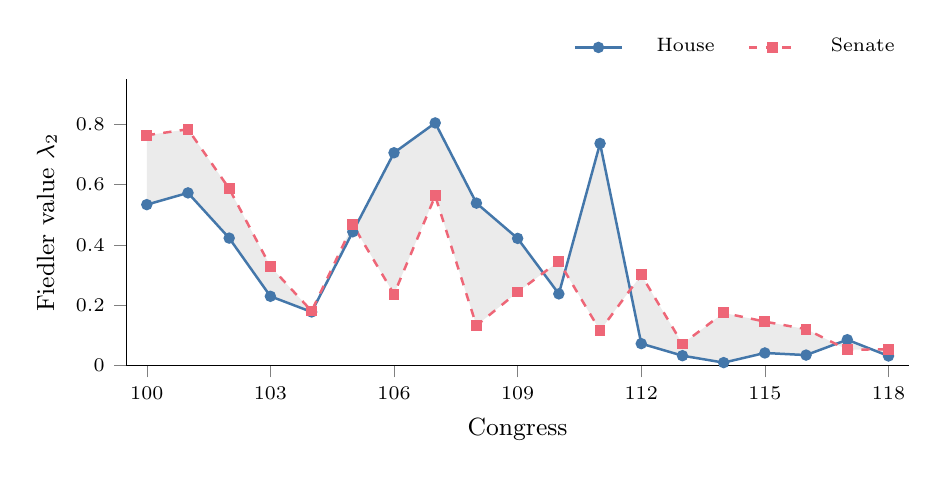
\begin{tikzpicture}
\begin{axis}[
  gat,
  width=0.82\linewidth, height=0.30\linewidth,
  xmin=99.5, xmax=118.5,
  ymin=0, ymax=0.95,
  ytick={0,0.2,0.4,0.6,0.8},
  xtick={100,103,106,109,112,115,118},
  xlabel={Congress},
  ylabel={Fiedler value $\lambda_2$},
  enlargelimits=false,
  legend style={at={(1.0,1.04)}, anchor=south east, font=\scriptsize, legend columns=2, column sep=10pt},
]

\addplot[name path=house, draw=none, forget plot] coordinates {
  (100,0.534) (101,0.573) (102,0.423) (103,0.230) (104,0.178)
  (105,0.444) (106,0.706) (107,0.805) (108,0.539) (109,0.422)
  (110,0.238) (111,0.737) (112,0.073) (113,0.033) (114,0.010)
  (115,0.042) (116,0.035) (117,0.086) (118,0.032)
};
\addplot[name path=senate, draw=none, forget plot] coordinates {
  (100,0.764) (101,0.784) (102,0.587) (103,0.329) (104,0.181)
  (105,0.467) (106,0.237) (107,0.563) (108,0.133) (109,0.244)
  (110,0.346) (111,0.116) (112,0.301) (113,0.072) (114,0.175)
  (115,0.146) (116,0.121) (117,0.053) (118,0.054)
};
\addplot[cgray!30, forget plot] fill between[of=house and senate];

\addplot[cblue, mark=*, mark size=1.6pt, mark options={fill=cblue, draw=cblue}]
  coordinates {
    (100,0.534) (101,0.573) (102,0.423) (103,0.230) (104,0.178)
    (105,0.444) (106,0.706) (107,0.805) (108,0.539) (109,0.422)
    (110,0.238) (111,0.737) (112,0.073) (113,0.033) (114,0.010)
    (115,0.042) (116,0.035) (117,0.086) (118,0.032)
  };
\addlegendentry{House}

\addplot[cred, mark=square*, mark size=1.5pt, dashed, mark options={solid, fill=cred, draw=cred}]
  coordinates {
    (100,0.764) (101,0.784) (102,0.587) (103,0.329) (104,0.181)
    (105,0.467) (106,0.237) (107,0.563) (108,0.133) (109,0.244)
    (110,0.346) (111,0.116) (112,0.301) (113,0.072) (114,0.175)
    (115,0.146) (116,0.121) (117,0.053) (118,0.054)
  };
\addlegendentry{Senate}

\end{axis}
\end{tikzpicture}
\caption{Fiedler value trajectories for the House and Senate co-voting networks, 100th--118th Congresses, both at the binary agreement threshold $\tau = 0.5$. The bicameral synthetic difference-in-differences of Section~\ref{sec:senate} re-estimates the Senate at $\tau = 0.6$. Shaded region marks the gap between the two chamber trajectories.}
\label{fig:bicameral}
\end{figure}

\section{Recovery Ratio Threshold Sensitivity}
\label{app:recovery}

Table~\ref{tab:recovery_sensitivity} reports structural recovery ratios at $\tau = 0.45$ and $\tau = 0.55$ alongside the primary $\tau = 0.50$ specification. The Contract with America recovery ratio ranges from 1.68 to 2.45 (full recovery at all thresholds), while the Tea Party ratio remains near zero (0.01--0.03) regardless of threshold. The qualitative contrast between the two episodes is robust.

\begin{table}[H]
\centering
\caption{Structural recovery ratio sensitivity to co-voting threshold $\tau$. Recovery ratio $R = \lambda_2(\text{post}) / \lambda_2(\text{pre})$.}
\label{tab:recovery_sensitivity}
\small
\begin{tabular}{lccccc}
\toprule
 & & \multicolumn{2}{c}{$\lambda_2$} & \\
\cmidrule(lr){3-4}
Shock & $\tau$ & Pre & Post & $R$ \\
\midrule
Contract with America & 0.45 & 0.376 (103rd) & 0.631 (105th) & 1.68 \\
 & 0.50 & 0.230 (103rd) & 0.444 (105th) & 1.93 \\
 & 0.55 & 0.112 (103rd) & 0.273 (105th) & 2.45 \\
\midrule
Tea Party Wave & 0.45 & 0.901 (111th) & 0.025 (114th) & 0.03 \\
 & 0.50 & 0.737 (111th) & 0.010 (114th) & 0.01 \\
 & 0.55 & 0.504 (111th) & 0.005 (114th) & 0.01 \\
\bottomrule
\end{tabular}
\end{table}

\section{Counterfactual Perturbation Sensitivity}
\label{app:counterfactual}

Table~\ref{tab:counterfactual_sensitivity} reports the Fiedler value of the 118th Congress network after adding cross-party edges to the $k$ most moderate members at rates calibrated to the 103rd Congress's cross-party agreement density (0.367 among moderates). The ``overlap'' column simulates committee overlap filtering: ``none'' adds edges to all eligible cross-party targets, ``loose'' (60\%) approximates any shared committee, and ``strict'' (30\%) approximates two or more shared committees. The baseline 118th Congress Fiedler value is 0.032.

\begin{table}[H]
\centering
\caption{Counterfactual edge-addition sensitivity. Perturbed Fiedler value of the 118th Congress network as a function of the number of moderates perturbed ($k$) and the stringency of the committee overlap filter.}
\label{tab:counterfactual_sensitivity}
\small
\begin{tabular}{lccccc}
\toprule
$k$ & Overlap & Edges Added & Perturbed $\lambda_2$ & Ratio vs.\ Base \\
\midrule
20 & none   & 1,298 & 0.065 & 2.1$\times$ \\
20 & loose  &   775 & 0.054 & 1.7$\times$ \\
20 & strict &   383 & 0.044 & 1.4$\times$ \\
\midrule
30 & none   & 2,071 & 0.086 & 2.7$\times$ \\
30 & loose  & 1,236 & 0.068 & 2.1$\times$ \\
30 & strict &   612 & 0.051 & 1.6$\times$ \\
\midrule
40 & none   & 2,857 & 0.108 & 3.4$\times$ \\
40 & loose  & 1,705 & 0.083 & 2.6$\times$ \\
40 & strict &   844 & 0.059 & 1.9$\times$ \\
\midrule
50 & none   & 3,651 & 0.130 & 4.1$\times$ \\
50 & loose  & 2,179 & 0.098 & 3.1$\times$ \\
50 & strict & 1,078 & 0.068 & 2.1$\times$ \\
\bottomrule
\end{tabular}
\end{table}

The qualitative result is robust: across all 12 specifications, the perturbed Fiedler value exceeds the baseline by at least 40\%, confirming that a small number of cross-partisan cooperators has outsized effects on algebraic connectivity. The magnitude varies roughly threefold across specifications, from a 1.4$\times$ improvement (20 members, strict overlap) to a 4.1$\times$ improvement (50 members, no overlap filter), supporting the range of 20--50 effective bridge legislators reported in the main text.

\section{Honest Difference-in-Differences Bounds}
\label{app:honest_did}

Table~\ref{tab:honest_did} reports honest difference-in-differences bounds for the cohort triple-difference event study of Section~\ref{sec:bli_departure}. The four pre-treatment coefficients in the cohort DDD event study at relative times $-5, -4, -3$, and $-2$ provide the pre-trend information that anchors the bounds. The relative-magnitudes restriction of \citet{rambachan2023honest} requires that post-treatment violations of parallel trends do not exceed $\bar{M}$ times the worst observed pre-period violation. At $\bar{M} = 0$ the bounds reproduce the original Callaway-Sant'Anna confidence set, and increasing $\bar{M}$ progressively relaxes the parallel-trends assumption. The point estimate at event time zero is 0.031, and the 95 percent C-LF (least favorable) confidence set at $\bar{M} = 0$ is $[-0.019, 0.081]$. The null is contained at every multiple of the worst pre-period violation, including $\bar{M} = 2$, where the bound is $[-0.160, 0.222]$.

\begin{table}[H]
\centering
\caption{Rambachan-Roth honest difference-in-differences bounds on the cohort DDD event-study coefficient at relative time 0. The original CS confidence set is reported for reference. $\bar{M}$ indexes the relative-magnitudes restriction.}
\label{tab:honest_did}
\small
\begin{tabular}{lcc}
\toprule
Restriction & Lower bound & Upper bound \\
\midrule
Original CS & $-0.020$ & $0.081$ \\
$\bar{M} = 0.00$ & $-0.019$ & $0.081$ \\
$\bar{M} = 0.25$ & $-0.028$ & $0.089$ \\
$\bar{M} = 0.50$ & $-0.040$ & $0.101$ \\
$\bar{M} = 1.00$ & $-0.075$ & $0.138$ \\
$\bar{M} = 1.50$ & $-0.117$ & $0.179$ \\
$\bar{M} = 2.00$ & $-0.160$ & $0.222$ \\
\bottomrule
\end{tabular}
\end{table}

The bounds contain zero across the full grid. The Tea Party wave at the 112th Congress yields only one pre-period after restricting to cycle-bounded observations, which is insufficient for HonestDiD identification, so we rely on the cohort DDD specification for the headline bound. The substantive interpretation is unchanged: the cohort triple difference does not detect a partisan-cohort effect on departure that exceeds plausible parallel-trends violations of up to twice the worst pre-period deviation.

\section{Sensitivity Battery for the BLI Departure Coefficient}
\label{app:sensitivity}

The Bridge Legislator Index coefficient in the OLS approximation of the GEE departure model is the load-bearing finding of Section~\ref{sec:bli_departure}. The coefficient is 39.1 without a centrism control and $-8.1$ with a centrism control, where the partial $R^2$ of BLI on departure falls from 0.0038 to 0.00012 with the centrism control added. We assess this finding from four directions: sensemakr robustness values, Oster $\delta^*$ proportional selection, the VanderWeele E-value, and a specification curve over 96 alternative model variants. We also report a causal forest of average and conditional effects.

Table~\ref{tab:sensemakr} reports the sensemakr robustness values for the no-centrism specification. The robustness value $RV_{q=1}$, the partial $R^2$ that an unobserved confounder would have to share with both treatment and outcome to fully reduce the BLI coefficient to zero, is 0.060. The three benchmark covariates (ideology distance from party median, seniority, and the Republican indicator) reach partial $R^2$ ratios of 0.052, 0.056, and 0.022, respectively, so an unobserved confounder roughly comparable to the strongest measured covariate is not sufficient to nullify the no-centrism BLI coefficient. The centrism-adjusted specification has $RV_{q=1} = 0.011$ and a partial $R^2$ of 0.00012, indicating that the conditional finding is fragile to any confounder of nontrivial strength.

\begin{table}[H]
\centering
\caption{Sensemakr robustness values for the BLI departure coefficient. $RV_{q=1}$ is the confounder partial $R^2$ required to reduce the coefficient to zero; $RV_{\alpha=0.05}$ is the partial $R^2$ required to make the coefficient statistically indistinguishable from zero at the 5 percent level.}
\label{tab:sensemakr}
\small
\begin{tabular}{lcc}
\toprule
Quantity & No centrism & With centrism \\
\midrule
BLI coefficient & 39.1 & $-8.1$ \\
Partial $R^2$ & 0.0038 & 0.00012 \\
$RV_{q=1}$ & 0.0598 & 0.0108 \\
$RV_{\alpha=0.05}$ & 0.0383 & --- \\
Benchmark ratio (ideology distance) & 0.052 & --- \\
Benchmark ratio (seniority) & 0.056 & --- \\
Benchmark ratio (Republican) & 0.022 & --- \\
\bottomrule
\end{tabular}
\end{table}

Table~\ref{tab:oster} reports the Oster $\delta^*$ bound for centrism treated as the omitted variable. The short regression coefficient on BLI is 39.1 and the long regression coefficient with centrism added is $-8.1$. The $R^2$ moves from 0.021 (short) to 0.035 (long). At $R^2_{\max}$ equal to 1.3 times the long $R^2$, the bias-adjusted coefficient at $\delta = 1$ is $-42.1$, and the $\delta^*$ that would set the bias-adjusted coefficient to zero is $-0.24$. Negative $\delta^*$ values are interpreted as ``the unobserved confounder must be negatively correlated with the observed controls in a direction opposite to selection on observables.'' The Oster diagnostic confirms that the centrism control is the active mediating variable in the departure regression, not a confounder: the sign of $\delta^*$ would be positive if BLI were independently associated with departure after conditioning on centrism.

\begin{table}[H]
\centering
\caption{Oster bias-adjusted coefficient bounds for the BLI departure coefficient with centrism as the omitted variable. $R^2_{\max}$ is reported as a multiplier on the long-regression $R^2$ (0.035).}
\label{tab:oster}
\small
\begin{tabular}{lcc}
\toprule
$R^2_{\max}$ multiplier & $\delta^*$ (bias = 0) & $\beta^*$ at $\delta = 1$ \\
\midrule
1.0$\times$ & --- & $-8.1$ \\
1.1$\times$ & $-0.71$ & $-19.4$ \\
1.3$\times$ & $-0.24$ & $-42.1$ \\
1.5$\times$ & $-0.14$ & $-64.8$ \\
2.0$\times$ & $-0.07$ & $-121.5$ \\
\bottomrule
\end{tabular}
\end{table}

The VanderWeele E-value provides a third independent assessment. On a risk-ratio scale, an interquartile-range increase in BLI is associated with a 1.29 risk ratio for departure given a base departure rate of 0.304. The E-value for the point estimate is 1.90, and for the lower confidence bound is 1.65. An unobserved confounder would have to be associated with both BLI and departure at a minimum risk ratio of 1.90 on the risk-ratio scale to fully account for the unconditional association. The threshold is moderate. The centrism variable in the adjusted model approaches this benchmark, which is the substantive finding rather than a robustness threat.

The specification curve over 96 alternative model variants (subsets of controls, era restrictions, alternative agreement thresholds, alternative outcome windows, and three GEE working correlations on the balanced subsample) returns a coefficient median of 30.4 with an interquartile range of $[12.0, 52.9]$. Sixty-six percent of specifications return statistically significant point estimates and 80 percent return positive signs. The full specification curve panel is shipped with the replication archive at \texttt{results/specification\_curve.csv}.

Table~\ref{tab:cforest} reports a generalized random forest of conditional average treatment effects with BLI as the treatment and departure as the outcome, evaluated on the 7,500 observation panel. The average treatment effect is $-19.7$ with a 95 percent confidence interval of $[-86.2, 46.8]$. The conditional average treatment effects vary by era: the early era (Congresses 100--105) carries a more negative effect of $-34.4$, while the middle era (106--110) and late era (111--116) attenuate to $-10.0$ and $-8.5$. Feature importance is dominated by absolute DW-NOMINATE position (0.48) and ideology distance from party median (0.31), consistent with the centrism story rather than an independent BLI channel.

\begin{table}[H]
\centering
\caption{Causal forest conditional average treatment effects with BLI as the continuous treatment and departure within two Congresses as the outcome.}
\label{tab:cforest}
\small
\begin{tabular}{lcc}
\toprule
Stratum & $N$ & CATE mean \\
\midrule
Full sample & 7,500 & $-19.7$ \\
Early era (100--105) & 3,077 & $-34.4$ \\
Middle era (106--110) & 2,658 & $-10.0$ \\
Late era (111--116) & 1,765 & $-8.5$ \\
Republicans & 3,654 & $-8.5$ \\
Democrats & 3,846 & $-30.3$ \\
\bottomrule
\end{tabular}
\end{table}

Taken together, the four sensitivity diagnostics support a single substantive reading. The unconditional BLI departure association is moderately robust to plausible confounders. The conditional association, after adjusting for centrism, is fragile to any nontrivial confounder. The empirical pattern is consistent with centrism acting as a mediator of BLI on departure rather than as a confounder, which matches the formal mediation analysis reported in Section~\ref{sec:bli_departure}.

\section{Centrality Benchmark}
\label{app:centrality}

Table~\ref{tab:centrality_comparison} reports the median Spearman correlation of each comparator centrality with the leave-one-out Bridge Legislator Index across the 19 Congresses in our panel. The comparators are betweenness, eigenvector, closeness, harmonic, PageRank, $k$-core, degree, and the dynamical importance index of \citet{restrepo2006characterizing}. The Bridge Legislator Index correlates negatively and strongly with dynamical importance (median $\rho = -0.93$), as expected: dynamical importance measures the rate of change of the leading eigenvalue under node perturbation, and the leave-one-out perturbation of the Fiedler value (the second-smallest eigenvalue of the normalized Laplacian) is the analogue we use for cooperative bridging rather than dominance.

\begin{table}[H]
\centering
\caption{Median Spearman correlation across 19 Congresses between leave-one-out Bridge Legislator Index and eight comparator centrality measures.}
\label{tab:centrality_comparison}
\small
\begin{tabular}{lc}
\toprule
Comparator & Median $\rho$ with BLI \\
\midrule
Dynamical importance & $-0.93$ \\
BLI (first-order approximation) & $-0.93$ \\
$k$-core & 0.57 \\
Betweenness & 0.89 \\
Eigenvector & 0.91 \\
Degree & 0.96 \\
Closeness & 0.96 \\
Harmonic & 0.96 \\
PageRank & 0.98 \\
\bottomrule
\end{tabular}
\end{table}

The conventional centralities (PageRank, degree, closeness, harmonic) correlate above 0.94 with BLI, which establishes that the bridge legislator ranking is not orthogonal to existing measures of network position but is also not redundant with them. Betweenness, the centrality most commonly invoked for ``brokerage'' in the political science literature, correlates at 0.89 median and as low as 0.76 in the 112th Congress, where partisan polarization is most acute. The substantive case for BLI over these alternatives rests on three properties: a closed-form linear approximation that supports inference (Theorem~\ref{thm:first_order}), submodularity of the bridge legislator set (Proposition~\ref{prop:submodular}), and a direct link to the algebraic connectivity that governs structural robustness. The first-order approximation $\rho = -0.93$ confirms that the closed form tracks the exact leave-one-out perturbation across the panel.

\section{Code and Data Availability}

All code, processed data, and figure generation scripts are publicly available at \url{https://github.com/human-vc/CongressNetwork}. The repository contains the full pipeline from raw Voteview downloads through spectral analysis, null model validation, and figure generation. Any researcher can verify, critique, or extend the analysis without relying on our word alone.

\end{document}
